\documentclass{article}
\usepackage[utf8]{inputenc}
\usepackage{amsmath}
\usepackage{amsfonts}
\usepackage{amssymb}
\usepackage{amsthm}
\usepackage{verbatim}
\usepackage{dsfont}

%Double spacing
\usepackage{setspace}
\doublespacing

%Theorems Environment
\newtheorem{theorem}{Theorem}[section]
\newtheorem{corollary}{Corollary}[theorem]
\newtheorem{lemma}[theorem]{Lemma}
\newtheorem{example}{Example}
\newtheorem*{remark}{Remark}
\theoremstyle{definition}
\newtheorem{definition}{Definition}[section]

\usepackage[colorlinks=true, allcolors=blue,bookmarks=true]{hyperref} %references

%Make tight space on edges for text
\usepackage{anysize}
%\marginsize{left}{right}{top}{botton}
\marginsize{1cm}{1cm}{1cm}{1cm}

%Commands    
\newcommand{\ip}[2]{\ensuremath{\left\langle{#1}\middle\vert{#2}\right\rangle}}
\newcommand{\expval}[1]{\ensuremath{\left\langle #1 \right\rangle}}
\newcommand{\op}[2]{\ensuremath{\left\vert{#1}\middle\rangle\middle\langle{#2}\right\vert}}

\usepackage{natbib} %Bibliography
\usepackage{graphicx} %images
\usepackage{float} %images to stay on place
% \usepackage[braket, qm]{qcircuit}
% \usepackage[qm]{qcircuit}
\usepackage{pgf,pgfplots}
\pgfplotsset{compat=1.15}
\usepackage{mathrsfs}

% Algorithms
\usepackage[ruled,vlined]{algorithm2e}

% Circle equations 
\usepackage{empheq}
\usepackage[most]{tcolorbox}

\usetikzlibrary{arrows}
\usepackage{tikz}
\usetikzlibrary{quantikz}
% Updated for remove warning
% \usepackage{circuitikz}
\usepackage[RPvoltages]{circuitikz}

\usepackage{sidecap}
\usepackage{epigraph}
\title{Notes on Quantum Computing}
\author{Nahum Sá}

\begin{document}

\maketitle
\begin{abstract}
    These are my notes about quantum computing.
\end{abstract}
\newpage
\tableofcontents
\newpage

% Quantum Information Chapter
\section{Quantum Information}
\label{Sec: Quantum Information}

\paragraph{}This will be a short introduction on quantum information in order to have a theoretical basis to understand most Quantum Algorithms.
\subsection{Postulates of Quantum Mechanics}
\label{Subsec: Postulates of Quantum Mechanics}
\paragraph{}As stated in Aaronson \cite{Aaronson:2013:QCD:2487754}, there are two ways of introducing quantum mechanics: The physicist's way explaining the history behind the discovery of quantum theory and stating postulates of quantum theory as an endpoint, or showing that quantum mechanics is a generalization of probability theory. Here I will take the physicist's position and skip the history stuff and introduce the postulates of quantum theory.

The quantum mechanics postulates are, according to Nielsen and Chuang \cite{nielsen_chuang_2010}: 
\begin{enumerate}
    \item Associated to any isolated physical system is a complex vector space with inner product (that is, a Hilbert space) known as the state space of the system. The system is completely described by its state vector, which is a unit vector in the system’s state space.
    \item The evolution of a closed quantum system is described by a unitary transformation. That is, the state \ket{\psi} of the system at time $t_1$ is related to the state \ket{\psi}  of the system at time $t_2$ by a unitary operator U which depends only on the times $t_1$ and $t_2$ , $\ket{\psi(t_2)} = U \ket{\psi(t_1)}$.
    \item Quantum measurements are described by a collection of POVMs $\{M_m\}$ of measurement operators. These are operators acting on the state space of the system being measured. The index m refers to the measurement outcomes  that  may occur in the experiment. If the state of the quantum system is \ket{\psi} immediately before the measurement then the probability that result m occurs  is given by:
    \begin{equation}
        p(m) = \bra{\psi} M_m^{\dagger} M_m \ket{\psi}
    \end{equation}
    And the system after the measurement is:
    \begin{equation}
        \frac{M_m \ket{\psi}}{\bra{\psi} M_m^{\dagger} M_m \ket{\psi}}
    \end{equation}
    Where $\sum_m M_m^{\dagger} M_m = \mathbb{I}$.
    
    \item The state space of a composite physical system is the tensor product of the state spaces of the component physical systems. Moreover, if we have systems numbered 1 through n: $\ket{\psi} = \ket{\psi_1} \otimes \ket{\psi_2} \dots \ket{\psi_n}$
\end{enumerate}

To sum up, the first postulate states that wave functions lives in Hilbert Space, the second one states that evolutions are unitary, the third one states that the wavefunction collapses when it's measured (For a good Everretian this might seems strange) and the final one states that composite systems are described by tensor products.
\subsection{Qubit}
\label{Subsec: Qubit}

\paragraph{}One qubit is a subspace with two dimensions, that means we can map a qubit to $\mathbf{C}^2$ . We can choose a basis in order to span this vector space, we will choose the standard computational basis that will be associated to bits:
\begin{equation}
\label{Eq: Computational Basis}
\ket{0} =  
\begin{pmatrix} 
1 \\
0 \\
\end{pmatrix}
\
and
\
\ket{1} =  
\begin{pmatrix} 
0 \\
1 \\
\end{pmatrix}
\end{equation}

The general state of a qubit is a superposition of those states:

\begin{equation}
\label{Eq: Superposition of qubit}
\ket{\psi} = \alpha \ket{0} + \beta \ket{1}
\end{equation}

This state can be parameterized by two parameters and construct what we call a "Bloch Sphere":
\begin{equation}
\label{Eq: Bloch Sphere}
\ket{\psi} = cos\left(\frac{\theta}{2} \right) \ket{0} + e^{i\phi}sin\left(\frac{\theta}{2} \right) \ket{1}
\end{equation}

\begin{figure}[H]
\centering
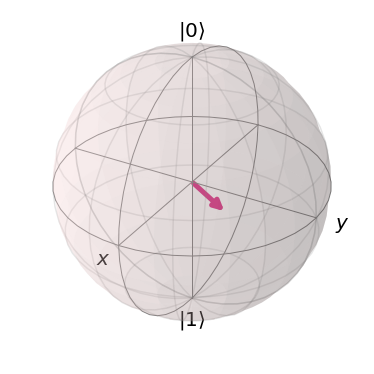
\includegraphics[width=0.3\textwidth]{Figures/bloch.png}
\caption{Graphical representation of the Bloch sphere.}
\end{figure}
\subsection{Density Matrix}
\label{Subsection: Density Matrix}
\paragraph{} Density matrix is a generalization of quantum states (For the sake of simplicity, some people call the density matrix of a system the state of a system, because we can always purify it, see Sec~\ref{Subsection: Purification}). I will introduce this concept with an example that will be easily generalized.

Consider that you send a state $\ket{+}$ with probability p and a state $\ket{0}$ with probability $(1-p)$, where: $\ket{+} = \frac{\ket{0} + \ket{1}}{\sqrt{2}}$, how would you describe this state as a ket? No!

Since you do not know which state came out exactly, you need to consider this uncertainty into our formulation, this is done using a density matrix $\rho$:
\begin{equation}
    \rho = p \ket{+} \bra{+} + (1-p) \ket{0} \bra{0} = \frac{p}{2}\begin{pmatrix}
     1 & 1 \\
     1 & 1
    \end{pmatrix} + (1-p) \begin{pmatrix}
    1 & 0 \\
    0 & 0
    \end{pmatrix} = \begin{pmatrix}
    1 - \frac{p}{2} & \frac{p}{2} \\
    \frac{p}{2} & \frac{p}{2}
    \end{pmatrix}
\end{equation}

Let's consider $p = \frac{1}{2}$: 

\begin{equation}
    \rho = \begin{pmatrix}
    \frac{3}{4} & \frac{1}{4} \\
    \frac{1}{4} & \frac{1}{4}
    \end{pmatrix}
\end{equation}

 
What is the probability to measure the state $\ket{0}$? 
 

By intuition since we have probability $\frac{1}{2}$  of finding the state on $\ket{+} = \frac{\ket{0} + \ket{1}}{\sqrt{2}}$  and probability $\frac{1}{2}$  of finding the state on $\ket{0}$, the probability of measuring $\ket{0}$ in the state $\ket{+}$ is $\frac{1}{2}$ given by the second postulate of quantum mechanics, therefore the probability is given by:

\begin{equation}
    p(0) = \frac{1}{2}\overbrace{\frac{1}{2}}^{\ket{+}} + \  \frac{1}{2}\overbrace{1}^{\ket{0}} = \frac{3}{4} = \bra{0} \rho \ket{0} = Tr(\rho \ket{0} \bra{0})
\end{equation}

 

\textbf{Exercise 1}: What is the probability of measuring the state \ket{1}?

 

\textbf{Exercise 2}: What is the probability of measuring the state \ket{1} or the state \ket{0}?

 

Now we can generalize what a density matrix is. Consider a quantum system with i states $\ket{\psi_i}$ with respective probabilities $p_i$. The density matrix of this system is given by:
\begin{equation}
    \label{Eq: Density Operator}
    \rho = \sum_i p_i \ket{\psi_i}\bra{\psi_i}
\end{equation}

The evolution of a quantum state is given by an unitary transformation U, then the evolution of the density matrix is given by:
\begin{equation}
    \rho = \sum_i p_i \ket{\psi_i}\bra{\psi_i} \xrightarrow{U} \sum_i p_i U\ket{\psi_i}\bra{\psi_i}U^{\dagger} = U \rho U^{\dagger}
\end{equation}

Measurements, as shown above, also can be generalized for the density operator formalism. Suppose the measurement operators $M_m$. If the initial state was $\ket{\psi_i}$, the probability of measuring m given i is:
\begin{equation}
    p(m|i) = \bra{\psi_i} M_m^{\dagger}M_m \ket{\psi_i} = Tr(M_m^{\dagger}M_m \ket{\psi_i}\bra{\psi_i})
\end{equation}

By the laws of probability:
\begin{equation}
    \begin{split}
        p(m) = & \ \sum_i p(m|i) p_i \\
        = & \ \sum_i p_i \ Tr(M_m^{\dagger}M_m \ket{\psi_i}\bra{\psi_i}) \\
        = & \ Tr( M_m^{\dagger}M_m \rho )
    \end{split}
\end{equation}

Therefore, if you want to know the value of any observable $A$, you have:
\begin{equation}
    \left<A\right> = Tr( A \rho )
\end{equation}

The class of operators that are density operators are characterized by the following useful theorem(From \citep{nielsen_chuang_2010}):

\begin{theorem}[Characterization of Density Operators]
An operator $\rho$ is the density operator associated to some ensemble \{ $p_i$ , $\ket{\psi_i}$ \} if and only if it satisfies the
conditions:

\begin{itemize}
    \item \textbf{Unity Trace}: $Tr(\rho) = 1$
    \item \textbf{Positivity}: $\rho \geq 0$
\end{itemize}
\end{theorem}

\begin{proof}
Suppose $\rho = \sum_i p_i \ket{\psi_i}\bra{\psi_i}$. Then
\begin{itemize}
    \item \textbf{Unity Trace}: 
    \begin{equation}
        Tr(\rho) = Tr(\sum_i p_i \ket{\psi_i}\bra{\psi_i}) = \sum_i p_i \overbrace{Tr(\ket{\psi_i}\bra{\psi_i})}^{=1} = \sum_i p_i = 1
    \end{equation}
    
    \item \textbf{Positivity}: Suppose $\ket{\phi}$ is an arbitrary state. Then:
    \begin{equation}
        \begin{split}
            \bra{\phi} \rho \ket{\phi} = & \ \sum_i p_i \braket{\phi}{\psi_i}\braket{\psi_i}{\phi} \\
            = & \ \sum_i p_i |\braket{\phi}{\psi_i}|^2 \\
            \geq &  \ 0
        \end{split}
    \end{equation}
\end{itemize}

Now suppose $\rho$ is an operator that the trace is unity and is positive. Since $\rho$ is positive, it must have a spectral decomposition:

\begin{equation}
    \rho = \sum_i \lambda_i \ket{i} \bra{i}
\end{equation}

From the unity of the trace, we have that $\sum_i \lambda_i = 1$. Therefore, we have the ensemble \{ $\lambda_i$ , $\ket{i}$ \} that gives rise to the density operator $\rho$.
\end{proof}
 
\textbf{Question}: Can we distinguish between two ensembles? 
 

No! For example the ensembles: 
\begin{enumerate}
    \item \{ ($\frac{1}{2}$, $\ket{0}$), ($\frac{1}{2}$, $\ket{1}$)  \} $\rightarrow$ \ $\rho = \frac{1}{2}( \ket{0} \bra{0} + \ket{0} \bra{0}) = \frac{\mathds{1}}{2}$ 
    \item \{ ($\frac{1}{2}$, $\ket{+}$), ($\frac{1}{2}$, $\ket{-}$)  \} $\rightarrow$ \ $\rho = \frac{1}{2}( \ket{+} \bra{+} + \ket{-} \bra{-}) = \frac{\mathds{1}}{2}$ 
\end{enumerate}
 
\textbf{Exercise}: Work out the details of the above ensembles.
 
We can discriminate between two types of states:

\begin{itemize}
    \item \textbf{Pure States}: States that we have complete knowledge.
    \begin{equation}
        \rho = \ket{\psi_i} \bra{\psi_i} \ , \ p_i =1 \ , \ p_{j \neq i} = 0
    \end{equation}
    \item \textbf{Mixed States}: States that we do not have complete knowledge.
    \begin{equation}
        \rho = \sum_i \ket{\psi_i} \bra{\psi_i} 
    \end{equation}
    With at least two $p_i$'s that are different than 0.
\end{itemize}

We can quantify the purity of a state using the following measure:

\begin{equation}
    P(\rho) = Tr(\rho^2)
\end{equation}

\textbf{Example 1} (Pure State): $\rho = \ket{\psi} \bra{\psi}$

\begin{equation}
    P( \ket{\psi} \bra{\psi} ) = Tr( (\ket{\psi} \bra{\psi}) ^2) = Tr( \ket{\psi} \overbrace{\bra{\psi} \ket{\psi}}^{=1} \bra{\psi}) = Tr( \ket{\psi} \bra{\psi} ) = 1
\end{equation}

 

\textbf{Example 2} (Mixed State): Since $\rho$ is hermitian we can consider its spectral decomposition $ \rho = \sum_i \lambda_i \ket{\phi_i} \bra{\phi_i} $, where $\braket{\phi_i}{\phi_j} = \delta_{ij}$, $\lambda_i \geq 0$ and $\sum_i \lambda_i = 1$. Therefore:

\begin{equation}
    P(\rho) = Tr((\sum_i \lambda_i \ket{\phi_i} \bra{\phi_i})^2) = Tr(\sum_i \sum_j \lambda_i \lambda_j \ket{\phi_i} \overbrace{\bra{\phi_i} \ket{\phi_j}}^{= \delta_{ij}} \bra{\phi_j}) = Tr( \sum_i \lambda_i^2 \ket{\phi_i} \bra{\phi_i}) = \sum_i \lambda_i^2 \leq 1
\end{equation}
 
\textbf{Exercise}: Find the purity of the maximally mixed state $\rho = \mathds{1}/d$, where d is the dimension of the finite Hilbert Space.
 

If you tried to do the exercise, you will find that the purity of a d-dimensional state lies between two fixed values $\frac{1}{d} \leq P(\rho) \leq 1$.

\subsection{Qubit Revisited}
\label{Subsection: Qubit Revisited}

In section~\ref{Subsec: Qubit} we introduced the concept of qubits, but we didn't have the density operator formalism yet, now we take a more detailed look on qubits and the bloch sphere.

The density matrix of a qubit is a $2\mathrm{x}2$ matrix: 
\begin{equation}
    \rho = \begin{pmatrix}
    \rho_{00} & \rho_{01} \\
    \rho_{10} & \rho_{11}
    \end{pmatrix} = \sum_{i=0}^1 \sum_{j=0}^1 \rho_{ij} \ket{i} \bra{j}
\end{equation}

Since it is a density matrix, we have that: $\rho_{00} + \rho_{11} = 1$ and $\rho_{ij}^* = \rho_{ji}$

We can expand the density matrix on the pauli matrices basis: $\mathcal{B}_{2\mathrm{x}2} = \{\mathds{1}, \sigma_x, \sigma_y, \sigma_z \}$.

The Pauli Matrices are: 

\begin{equation}
    \sigma_x = \begin{pmatrix}
    0 & 1 \\
    1 & 0
    \end{pmatrix} \hspace{1em} , \hspace{1em}  \sigma_y = \begin{pmatrix}
    0 & -i \\
    i & 0
    \end{pmatrix} \hspace{1em} , \hspace{1em}  \sigma_z = \begin{pmatrix}
    1 & 0 \\
    0 & -1
    \end{pmatrix}
\end{equation}

And they have the following properties:
\begin{itemize}
    \item Hermitian: $\sigma_i = \sigma_i^{\dagger}$, $\forall i$ ;
    \item $Tr(\sigma_i) = 0$, $\forall i \in \{x,y,z \}$ ;
    \item $Tr(\sigma_i^{\dagger} \sigma_j) = 2 \delta_{ij}$ ;
    \item $\sigma_i \sigma_j = \delta_{ij} \mathds{1} + i  \epsilon_{ijk} \sigma_k$, $i,j,k \in \{x,y,j \}$, in particular $\sigma_i^2 = \mathds{1}$.
\end{itemize}

Writing the qubit on the Pauli Matrices basis, we have:

\begin{equation}
    \rho = r_0 \mathds{1} + r_1 \sigma_x + r_2 \sigma_y + r_3 \sigma_z
\end{equation}

Applying the unit trace condition, we have:

\begin{equation}
    Tr(\rho) = 1 \Rightarrow 2 r_0 = 1 \Rightarrow r_0 = \frac{1}{2}
\end{equation}

Therefore:

\begin{equation}
    \rho = \frac{1}{2} \mathds{1} + r_1 \sigma_x + r_2 \sigma_y + r_3 \sigma_z
\end{equation}

Using that the density matrix is Hermitian, we have that:

\begin{equation}
    \rho = \rho^{\dagger} \Rightarrow \frac{1}{2} \mathds{1} + r_1 \sigma_x + r_2 \sigma_y + r_3 \sigma_z = \frac{1}{2} \mathds{1} + r_1^* \sigma_x + r_2^* \sigma_y + r_3 \sigma_z^* \Rightarrow r_1,r_2,r_3 \in \mathds{R}
\end{equation}

We choose $r_1 = \frac{1}{2} r_x$, $r_2 = \frac{1}{2} r_y$, $r_3 = \frac{1}{2} r_z$, then our qubit density matrix is written as: 

\begin{equation}
    \label{Eq: Qubit Density Matrix}
    \rho = \frac{1}{2} \bigg( \mathds{1} + r_x \sigma_x + r_y \sigma_y + r_z \sigma_z \bigg) = \frac{1}{2} \bigg( \mathds{1} + \mathbf{r} \cdot \mathbf{\sigma} \bigg)
\end{equation}

Writing as a matrix, we have:

\begin{equation}
    \rho = \frac{1}{2} \begin{pmatrix}
    1 + r_z & r_x - i r_y \\
    r_x + i r_y & 1 - r_z
    \end{pmatrix}
\end{equation}

So now, in order to know where the state is in the Bloch sphere we just write the density matrix and find $r_x,r_y \ \mathrm{and} \ r_z $. 

It is interesting to note that pure and mixed states stay on different regions of the Bloch sphere, let's calculate the purity of an generic qubit:

\begin{equation}
    \begin{split}
        P(\rho) & = Tr(\rho^2) = Tr \bigg[ \bigg( \frac{1}{2} ( \mathds{1} + \mathbf{r}\cdot\mathbf{\sigma} \bigg)^2 \bigg] 
         = \frac{1}{4} \ Tr \bigg(\mathds{1} + \mathbf{r}\cdot\mathbf{\sigma} \bigg)\bigg(\mathds{1} + \mathbf{r}\cdot\mathbf{\sigma} \bigg) \\
        & = \frac{1}{4} \ Tr \bigg( \mathds{1} + 2 \mathbf{r}\cdot\mathbf{\sigma} + \sum_{ij} r_i r_j \sigma_i \sigma_j \bigg) \\
        & = \frac{1}{4} \ Tr \bigg( \mathds{1} + 2 \mathbf{r}\cdot\mathbf{\sigma} + \sum_{i \neq j} r_i r_j \sigma_i \sigma_j + \sum_{i } r_i^2  \overbrace{\sigma_i^2}^{=\mathds{1}} \bigg) \\
        & = \frac{1}{4} ( 2 + 2 \sum_i r_i^2) = \frac{1}{2} ( 1 + |\mathbf{r}|^2)
    \end{split}
\end{equation}

Therefore we have two situations:
\begin{itemize}
    \item Pure States: If $|\mathbf{r}|=1$, therefore it is in the spherical shell.
    \item Mixed States: If $|\mathbf{r}|<1$, those states are inside the Bloch sphere in a spherical shell("isopure shells").
\end{itemize}
\subsection{Purification}
\label{Subsection: Purification}
\paragraph{} Given a density matrix $\rho_A \in \mathcal{L}(\mathcal{H}_A)$, there always is an pure state $\ket{\psi_{AB}} \in \mathcal{H}_A \otimes \mathcal{H}_B$ such that: $\rho_A = Tr_B (\ket{\psi_{AB}}\bra{\psi_{AB}})$. 

For instance, consider $\rho_A = \sum_{i=1}^N p_i \ket{\phi_i}\bra{\phi_i}$ with $p_i \geq 0$ and $\sum_{i=1}^N p_i = 1$. We can suppose that there is an orthonormal basis $\{\ket{i} \}_{i=1}^N \in \mathcal{H}_B$, then we can take the pure state as:
\begin{equation}
    \ket{\psi_{AB}} = \sum_{i=1}^N \sqrt{p_i} \ket{\phi_i} \otimes \ket{i}
\end{equation}

Checking that this is a purification of $\rho_A$:
\begin{equation}
    \begin{split}
        Tr_B (\ket{\psi_{AB}}\bra{\psi_{AB}}) & = Tr_B \big\{ \sum_{i,j} \sqrt{p_i p_j} \ket{\phi_i}\bra{\phi_j} \otimes \ket{i}\bra{j} \big\} \\
        & = \sum_{i,j} \sqrt{p_i p_j} \ket{\phi_i}\bra{\phi_j} \overbrace{Tr \big(\ket{i}\bra{j}\big)}^{\delta_{ij}} \\
        & = \sum_i p_i \ket{\phi_i}\bra{\phi_i} \\
        & = \rho_A
    \end{split}
\end{equation}

It is important to note that there are infinite purifications for the density matrix $\rho_A \in \mathcal{L}(\mathcal{H}_A)$. 

\begin{theorem}[Non unicity of purifications]
If $\ket{\psi_{AB}}$ is such that $\rho_A = Tr_B (\ket{\psi_{AB}}\bra{\psi_{AB}})$, then $\mathds{1} \otimes U_B \ket{\psi_{AB}}$ is also a valid purification with $U_B^{\dagger}U_B = \mathds{1}$.
\end{theorem} 

\begin{proof}
Suppose that $\rho_A = Tr_B (\ket{\psi_{AB}}\bra{\psi_{AB}})$, then:
\begin{equation}
\begin{split}
    & Tr_B \big \{ (\mathds{1} \otimes U_B) \ket{\psi_{AB}}\bra{\psi_{AB}} (\mathds{1} \otimes U_B^{\dagger}) \big \} =\\
    & Tr_B \big \{  \ket{\psi_{AB}}\bra{\psi_{AB}} (\mathds{1} \otimes U_B^{\dagger}) (\mathds{1} \otimes U_B) \big \} =\\
    & Tr_B (\ket{\psi_{AB}}\bra{\psi_{AB}}) = \rho_A
\end{split}
\end{equation}
Where we used the cyclic property of the trace.
\end{proof}
% \subsection{Fidelity}
\label{Subsection: Fidelity}
% \subsection{POVM}
\label{Subsection: POVM}
\subsection{Entanglement}
\label{Subsection: Entanglement}

\begin{definition}[Product State]
A given state $\ket{\psi} \in \mathcal{H}_A \otimes \mathcal{H}_B$ is said to be a product state if $\exists \ket{\phi} \in \mathcal{H}_A$ and $\exists \ket{\chi} \in \mathcal{H}_B$, such that: $\ket{\psi} = \ket{\phi} \otimes \ket{\chi}$.
\end{definition}

\textbf{Example 1} \ (Product State): Consider the following state:

\begin{equation}
    \begin{split}
    \ket{\psi} =  & \frac{1}{2}\bigg(\ket{00} + \ket{01} \bigg) \\
    = & \frac{1}{2}\bigg(\ket{0} \otimes(\ket{0} + \ket{1})) \bigg)
    \end{split}
\end{equation}

\begin{definition}[Entangled State]
A given state $\ket{\psi} \in \mathcal{H}_A \otimes \mathcal{H}_B$ is said to be entangled if $\nexists \ket{\phi} \in \mathcal{H}_A$ and $\nexists \ket{\chi} \in \mathcal{H}_B$, such that: $\ket{\psi} = \ket{\phi} \otimes \ket{\chi}$.
\end{definition}

\textbf{Example 1} \ (Entangled State): Consider the following state:

\begin{equation}
    \begin{split}
    \ket{\psi} =  & \frac{1}{2}\bigg(\ket{00} + \ket{01} + \ket{10} - \ket{11} \bigg) \\
    = & \frac{1}{2}\bigg(\ket{0} \otimes(\ket{0} + \ket{1}) + \ket{1}\otimes(\ket{0} - \ket{1}) \bigg)
    \end{split}
\end{equation}
\subsection{No-go Theorems}
\label{Subsec: No-go Theorems}

\subsubsection{No communication Theorem}
\label{Subsubsec: No Comunication theorem}

\paragraph{}Consider that you have a composite physical system with $\mathcal{H} = \mathcal{H}_A \otimes \mathcal{H}_B$ and those states are finite dimensional. A general state on $\mathcal{H}$ is given by: $\rho = \sum_i \sigma_i \otimes \omega_i$, where $\sigma_i \in \mathcal{L}(\mathcal{H}_A)$ and $\omega_i \in \mathcal{L}(\mathcal{H}_B)$.

The observer in A makes a measurement only on her subsystem:

\begin{equation}
    P(\rho) = \sum_j (K_j \otimes \mathds{1}_B)^{\dagger} \rho (K_j \otimes \mathds{1}_B)
\end{equation}

Where $K_j$ are Kraus Operators(See~\ref{Subsec: Channels}) with the property: $\sum_j K_j K_j^{\dagger} = \mathds{1}$.

Now the state for an observer in B is given by the partial trace over A: 
\begin{equation}
    \rho_B = Tr_A (P(\rho))
\end{equation}

So let's see if there is any difference on the B state:

\begin{equation}
    \begin{split}
        \rho_B & = Tr_A ( \sum_j (K_j \otimes \mathds{1}_B)^{\dagger} \rho (K_j \otimes \mathds{1}_B) ) \\
        & = Tr_A(\sum_i \sum_j K_j^{\dagger} \sigma_i K_j \otimes \omega_i) \\
        & = \sum_i \sum_j Tr(K_j^{\dagger} \sigma_i K_j) \otimes \omega_i \\
        & = \sum_i Tr( \overbrace{\sum_j K_j K_j^{\dagger}}^{= \mathds{1}} \sigma_i) \otimes \omega_i \\
        & = \sum_i Tr(\sigma_i) \otimes \omega_i \\
        & = Tr_A(\rho)
    \end{split}
\end{equation}

Since the state before and after the local operations are indistinguishable for B, an observer in A doesn't have a way to communicate with and observer in B by using local operations. \textbf{There is no faster than light communication on Quantum Mechanics!}.


\subsubsection{No Cloning Theorem}
\label{Subsubsec: No Cloning theorem}

\begin{theorem}[No cloning Theorem]
There is no unitary U acting on $\mathcal{H} \otimes \mathcal{H}$ such that for all $\ket{\phi} \in \mathcal{H}$ we have:

\begin{equation}
    \label{Eq: No cloning theorem}
    U \ket{\phi} \otimes \ket{0} = \ket{\phi} \otimes \ket{\phi}
\end{equation}
\end{theorem}

This theorem can be represented by the following circuit:
\begin{figure}[H]
\centering
\begin{quantikz}
    \lstick{$\ket{\phi}$}   & \gate[wires=2]{U} &  \rstick{$\ket{\phi}$} \qw \\
    \lstick{$\ket{0}$}  &  & \rstick{$\ket{\phi}$} \qw
\end{quantikz}    
\caption{No-Cloning Theorem Circuit}
\label{Figure: Circuit No-Cloning Theorem}
\end{figure}

\begin{proof}
This theorem is proved by contradiction. Suppose that exists this unitary, so given $\ket{\phi}, \ket{\psi} \in \mathcal{H}$, we have that:

\begin{equation}
\begin{split}
    U \ket{\phi} \otimes \ket{0} & = \ket{\phi} \otimes \ket{\phi} \\ 
    U \ket{\psi} \otimes \ket{0} & = \ket{\psi} \otimes \ket{\psi}
\end{split}
\end{equation}

Taking the scalar product: 

\begin{equation}
    \begin{split}
        (\bra{\phi} \otimes \bra{\phi}) (\ket{\psi} \otimes \ket{\psi}) & =( \bra{\phi} \otimes \bra{0} U^\dagger)  (U \ket{\psi} \otimes \ket{0}) \\
        \braket{\phi}{\psi}\braket{\psi}{\phi} & = \braket{\phi}{\psi} \braket{0}{0}\\
        \Rightarrow \braket{\phi}{\psi}^2 & = \braket{\phi}{\psi}
    \end{split}
\end{equation}

This is a equation $x^2 - x = 0$, so there are two possible solutions: 

\begin{itemize}
    \item  $\braket{\phi}{\psi} = 0$, therefore $\ket{\phi}$, $\ket{\psi}$ are ortogonal;
    \item $\braket{\phi}{\psi} = 1$, therefore $\ket{\phi}$, $\ket{\psi}$ are identical;
\end{itemize}

This is a contradiction, because we supposed that U would work for every state.

\end{proof}

The No-Cloning theorem is really important in Quantum Cryptography. Because you cannot clone quantum states, it is impossible for a eavesdropper to hear your communication without you knowing. See BB84 Protocol~\citep{BB84}.

%\subsubsection{No Deleting Theorem}
%\label{Subsubsec: No Deleting Theorem}
\subsection{Channels}
\label{Subsec: Channels}
\paragraph{}Suppose a system with an environment state on a global unitary $U: \mathcal{H}_A \otimes \mathcal{H}_B \rightarrow \mathcal{H}_A \otimes \mathcal2{H}_B$:

\begin{figure}[H]
\centering
\begin{quantikz}
    \lstick{$\rho_a$}   & \gate[wires=2]{U} &  \rstick{$\Lambda(\rho_a)$} \qw \\
    \lstick{$\proj{0}_E$}  &  &  \qw
\end{quantikz}
= \ \  \begin{quantikz}
\lstick{$\rho_a$}   & \gate{\Lambda} &  \rstick{$\Lambda(\rho_a)$} \qw 
\end{quantikz}
\caption{Representation of quantum channels.}
\label{Figure: Circuit Quantum Channels}
\end{figure}

So we throw away the E part because we are only interested on part A. Therefore we will trace out the environment E:
\begin{equation}
    \label{Eq: Channel Definition}
    \lambda(\rho_A) = Tr_B (U \rho_A \otimes \proj{0}_E U^\dagger)
\end{equation}

Let's derive the formula for this channel:

\begin{equation}
    \label{Eq: U (Channel)}
    U = \sum_{k,l,m,n} U^{kl}_{mn} \op{kl}{mn}
\end{equation}

Using equation~\ref{Eq: U (Channel)} on equation~\ref{Eq: Channel Definition}:

\begin{equation}
\begin{split}
\Lambda(\rho_A) = &  \sum_i ( \mathds{1} \otimes \bra{i}) \left[ \sum_{k,l,m,n} U^{kl}_{mn} \op{kl}{mn}(\rho_A \otimes \op{0}{0}_E) \left( \sum_{r,s,p,q} U^{rs}_{pq} \op{rs}{pq} \right)^\dagger \right] ( \mathds{1} \otimes \ket{i}) \\
 = & \sum_i ( \mathds{1} \otimes \bra{i}) \left[ \sum_{k,l,m,n} U^{kl}_{mn} \op{kl}{mn}(\rho_A \otimes \op{0}{0}_E) \left( \sum_{r,s,p,q} (U^{rs}_{pq})^{*} \op{pq}{rs} \right) \right] ( \mathds{1} \otimes \ket{i}) \\ 
 = & \sum_i \sum_{k,l,m,n} \sum_{r,s,p,q} U^{kl}_{mn} (U^{rs}_{pq})^{*} \op{k}{m}\rho_A\op{p}{r} \otimes  \ip{i}{l} \ip{n}{0} \ip{0}{q}\ip{s}{i} \\
 = & \sum_i \sum_{k,m} \sum_{r,p} U^{ki}_{m0} (U^{ri}_{p0})^{*} \op{k}{m}\rho_A\op{p}{r} \\
 = & \sum_i \left( \sum_{k,m} U^{ki}_{m0} \op{k}{m} \right) \rho_A \left( \sum_{r,p} U^{ri}_{p0} \op{p}{r} \right)^\dagger \\
 \equiv & \sum_i K_i \rho_A K_i^\dagger
\end{split}
\end{equation}

Then we define the Kraus Operator $K_i : \mathcal{H}_A \rightarrow \mathcal{H}_A$:

\begin{equation}
    \label{Eq: Kraus Operator}
    K_i = \sum_{k,m} U^{ki}_{m0} \ \op{k}{m} = \bra{i}_E U \ket{0}_E
\end{equation}

Properties of quantum channels:
\begin{itemize}
    \item Linearity: 
    \begin{equation}
        \Lambda(\sum_j p_j \rho_j) = \sum_i K_i (\sum_j p_j \rho_j) K_i^\dagger = \sum_j \left( \sum_i K_i \rho_j K_i^\dagger \right) = \sum_j p_j \Lambda(\rho_j)
    \end{equation}
    
    
    \item Preserves Hermicity: If $\rho = \rho^\dagger \Rightarrow \Lambda(\rho)^\dagger = \Lambda(\rho)$
    
    \begin{equation}
        \Lambda(\rho)^\dagger = \left( \sum_i K_i \rho K_i^\dagger\right) ^\dagger =  \sum_i K_i \rho K_i^\dagger = \Lambda(\rho)
    \end{equation}
    \item Preserves the Trace:
    
    \begin{equation}
        Tr(\Lambda(\rho)) = Tr(\sum_i K_i \rho K_i^\dagger) = Tr(\sum_i K_i^\dagger K_i \rho)
    \end{equation}
    
    Using $K_i = \bra{i}_B U \ket{0}_B$, we have that:
    
    \begin{equation}
        \sum_i K_i^\dagger K_i = \sum_i \bra{0}_B U^\dagger \ket{i}_B  \bra{i}_B U \ket{0}_B =  \bra{i}_B U^\dagger U \ket{0}_B = \bra{i}_B \ket{0}_B = \mathds{1}_A 
    \end{equation}
    
    Therefore: 
    
    \begin{equation}
        Tr(\Lambda(\rho)) = Tr(\rho)
    \end{equation}
    
    \item Preserves Positivity: $\rho \geq 0 \Rightarrow \Lambda(\rho) \geq 0$
    \begin{equation}
        \Lambda(\rho) = \sum_i K_i \rho K_i^\dagger = \sum_i K_i \sqrt{\rho} \sqrt{\rho} K_i^\dagger
    \end{equation}
    
    Then, $\forall \ket{\psi}$: 
    \begin{equation}
        \bra{\psi} \Lambda(\rho) \ket{\psi} = \sum_i \bra{\psi} K_i \sqrt{\rho} \sqrt{\rho} K_i^\dagger \ket{\psi} = \sum_i || \sqrt{\rho} K_i \ket{\psi} || \geq 0
    \end{equation}
    
\end{itemize}

But in order to define an physically valid quantum channel, we have that the channel must return states even when applied to subsystems.

Channels which $\forall n \in \mathbb{N}: \Lambda \otimes \mathds{1}_n(\rho) \geq 0$ are said to be Completely Positive Maps.
\subsection{Quantum Measures}
\label{Subsection: Quantum Measures}

\subsubsection{Trace Distance}
\label{Subsubsec: Trace distance}

Trace distance can be interpreted as the probability of distinguishing between two density matrices. It is defined as the Schatten Norm for p=1:

\begin{equation}
    T(\rho,\sigma) = \frac{1}{2} || \rho - \sigma ||_1 = \frac{1}{2} \mathrm{Tr} \bigg[\sqrt{(\rho - \sigma)^{\dagger} (\rho - \sigma)} \bigg]
\end{equation}

Since density matrices are Hermitian, we have that:

\begin{equation}
    T(\rho, \sigma) = \frac{1}{2} \mathrm{Tr} \bigg[\sqrt{(\rho - \sigma)^2} \bigg] = \frac{1}{2} \sum_i \lambda_i
\end{equation}

Where $\lambda_i$ are the eigenvalues of ($\rho - \sigma$).

Properties \cite{nielsen_chuang_2010}:
\begin{itemize}
    \item Is a metric on the space of density matrices. 
    \item $0 \leq T(\rho, \sigma) \leq 1$ and $T(\rho,\sigma) = 1$ iff $\rho$ and $\sigma$ are orthogonal.
    \item It is Preserved under unitary transformations: $T(U\rho U^\dagger,U\sigma U^\dagger) = T(\rho, \sigma)$.
    \item It is convex in each of its inputs. $T(\rho,\sum_i p_i \sigma_i) \leq \sum_i p_i T(\rho,\sigma_i)$.
\end{itemize}

\subsubsection{Von Neumann Entropy}
\label{Subsubsec: Von Neumann entropy}

Von Neumann entropy of quantum state $\rho$ is defined as:

\begin{equation}
    S(\rho) \equiv - \mathrm{Tr}(\rho \mathrm{log} \rho)
\end{equation}

If $\lambda_x$ are the eigenvalues of $\rho$, then von Neumann's entropy definition can be re-expressed as:

\begin{equation}
    S(\rho) = - \sum_x \lambda_x \mathrm{log} \lambda_x
\end{equation}

And we define $0\mathrm{log}0 \equiv 0$.

\subsubsection{Quantum relative entropy}
\label{Subsubsec: Quantum Relative entropy}

The Von Neumann Entropy of a density matrix is $S(\rho) = - \mathrm{Tr} \ \rho \ \mathrm{log}\rho$, then we can define the quantum relative entropy between two density matrices $\rho$ and $\sigma$ as \cite{vedral2002role}, \cite{nielsen_chuang_2010}:

\begin{equation}
    S(\rho || \sigma) = - \mathrm{Tr} \big[ \rho \ \mathrm{log}\sigma \big] - S(\rho) = \mathrm{Tr} \big[ \ \rho \ \mathrm{log}\rho \big] - \mathrm{Tr} \big[ \ \rho \ \mathrm{log}\sigma \big] = \mathrm{Tr} \big[\ \rho ( \ \mathrm{log}\rho - \ \mathrm{log}\sigma) \big]
\end{equation}

This can be used as an entanglement measurement, consider a composite finite Hilbert space $H = \bigotimes_k H_k$, the relative entropy of entanglement of $\rho$ is defined by:

\begin{equation}
    D_{\mathrm{REE}}(\rho) = \min_{\sigma} S(\rho || \sigma)
\end{equation}
The minimum is taken over the family of separable states ($\rho = \sum_{i,j} p_{ij} \sigma_i \otimes \sigma_j$). We can intepret this as the quantity of distinguishability of the state $\rho$ from separable states. When $D_{REE} = 0$ we have a separable state, because of Klein's inequality.

\begin{theorem}[Klein's Inequality]

\begin{equation}
    S(\rho || \sigma) \geq 0 \ \mathrm{and} \ S(\rho || \sigma) = 0 \iff \rho = \sigma
\end{equation} 
\end{theorem}
\begin{proof}{\cite{nielsen_chuang_2010}}
Let $\rho = \sum_i p_i \op{i}{i}$ and $\sigma = \sum_j q_j \op{j}{j}$ be the orthonormal compositions for $\rho$ and $\sigma$.
From the definition, we have that:

\begin{equation}
    S(\rho||\sigma) = \sum_i p_i \mathrm{log} p_i - \sum_i \bra{i}\rho \mathrm{log}\sigma \ket{i}
\end{equation}
Let's simplify $\bra{i}\rho \mathrm{log}\sigma \ket{i}$:
\begin{equation}
    \bra{i}\rho \mathrm{log}\sigma \ket{i} = \bra{i}\bigg( \sum_j \mathrm{log}(q_j) \op{j}{j} \bigg)\ket{i} = \sum_i \mathrm{log}(q_j) P_{ij}
\end{equation}
Therefore, for the relative entropy, we have:

\begin{equation}
    S(\rho||\sigma) = \sum_i p_i \mathrm{log} p_i - \sum_i \sum_j p_i \mathrm{log}(q_j) P_{ij} = \sum_i p_i \bigg( \mathrm{log} (p_i) - \sum_j \mathrm{log}(q_j) P_{ij} \bigg)
\end{equation}
Note that the matrix $P_{ij}$ has double stochasticity ( $\sum_i P_{ij} = 1$ and $\sum_j P_{ij} = 1$ ) and $P_{ij} \geq 0$. Because log is a strictly concave function we have that $\sum_j P_{ij} \mathrm{log}(q_j) \leq log(r_i)$, where $r_i \equiv \sum_j P_{ij} q_j$ with equality iff $\exists j : P_{ij} =1$. Therefore:

\begin{equation}
    S(\rho||\sigma) \geq \sum_i p_i \mathrm{log} \frac{p_i}{r_i}
\end{equation}
With the equality iff for each $i$ there exists an $j$ such that $P_{ij} = 1$, that is iff $P_{ij}$ is a permutation matrix. This has the same form of the classical relative entropy, we have that:

\begin{equation}
    S(\rho||\sigma) \geq 0
\end{equation}

With equality iff $p_i = r_i \ \forall i$ and $P_{ij}$ is a permutation matrix. For this condition we can relabel the eigenstates of $\sigma$ such that $P_{ij}$ becomes the identity matrix, therefore $\rho$ and $\sigma$ are diagonal on the same basis and have the same eigenvalues, thus $\rho = \sigma$ iff $S(\rho||\sigma) = 0$. \qedsymbol
\end{proof}


\subsubsection{Quantum mutual information}
\label{Subsubsec: Quantum mutual information}

Consider a bipartite quantum system $H_{AB} = H_A \otimes H_B$ and let $\rho_{AB} \in \mathcal{L}(H_{AB})$. As defined on section~\ref{Subsubsec: Quantum Relative entropy}, the Von Neumann Entropy is $S(\rho) = - \mathrm{Tr} \ \rho \ \mathrm{log}\rho$. The reduced state of $\rho_{AB}$ on a subsystem $A$ is given by the partial trace: $\rho^A = \mathrm{Tr}_B \rho_{AB}$. The reduced Von Neumann Entropy is given by $S(\rho^A)$. Now the Quantum mutual informatin is defined is:

\begin{equation}
    I(A:B) = S(\rho^A) + S(\rho^B) - S(\rho^{AB}) = S(\rho^{AB} || \rho^A \otimes \rho^B)
\end{equation}
Where $S(\cdot || \cdot)$ is the quantum relative entropy (Sec~\ref{Subsubsec: Quantum Relative entropy}).

\newpage

% Quantum Computing Chapter
\section{Quantum Computing}
\label{Sec: Quantum Computing}
\paragraph{}Now we will focus on Quantum Computing and Algorithms for the Circuit model.
\subsection{Quantum Gates}
\label{subsec: Quantum Gates}

\subsubsection{One Qubit Gates}
\label{Subsubsec: One Qubit Gates}

\paragraph{}Since everything must be done in the realm of Quantum Mechanics the one qubit gates should be unitary 2x2 matrices, following the 2nd postulate.

The first gate is the \textit{Hadamard Gate}, defined as the matrix:

\begin{equation}
    H = \frac{1}{\sqrt{2}} \begin{pmatrix}
    1 & 1 \\
    1 & -1
    \end{pmatrix}
\end{equation}

This gate changes the computational basis $\{0,1 \}$ (Z basis) to a new basis: $\{ +,- \}$ (X basis).

\begin{equation}
    \begin{split}
        H \ket{0} = \frac{1}{\sqrt{2}} \big( \ket{0} + \ket{1} \big)  \equiv \ket{+} \\
        H \ket{0} = \frac{1}{\sqrt{2}} \big( \ket{0} - \ket{1} \big)  \equiv \ket{-}
    \end{split}
\end{equation}

Another important property of the Hadamard gate is that $H^2 = \mathds{1}$, so the inverse transformation is the Hadamard gate itself, $H^{\dagger} = H$.

The next gate is the \textit{Phase Shift Gate}:

\begin{equation}
R_z (\delta) = \begin{pmatrix}
1 & 0 \\
0 & e^{i \delta}
\end{pmatrix}
\end{equation}

This gate adds a phase only if the state is $\ket{1}$, Therefore for a general state $\ket{\psi} = \alpha \ket{0} + \beta \ket{1}$ with $|\alpha|^2 + |\beta|^2 = 1$:

\begin{equation}
    R_z (\delta) \ket{\psi} =  \alpha \ket{0} + e^{i \delta} \beta \ket{1}
\end{equation}

Since this is a relative phase, it is observed when you measure on the Z basis.

It is important to notice that every single qubit unitary operation can be made by only Phase Shift and Hadamard Gates:

For instance:

\begin{equation}
    R_z (\frac{\pi}{2} + \phi) H R_z(\theta) H \ket{0} = e^{i \frac{\theta}{2}} \big( cos\frac{\theta}{2} \ket{0} + e^{i\phi} \ket{1} \big)
\end{equation}

Let's show this:

\begin{equation}
\begin{split}
    R_z (\frac{\pi}{2} + \phi) H R_z(\theta) H \ket{0}  = & R_z (\frac{\pi}{2} + \phi) H R_z(\theta) \frac{1}{\sqrt{2}} \big( \ket{0} + \ket{1} \big) \\
    = & R_z  (\frac{\pi}{2} + \phi) H \frac{1}{\sqrt{2}} \big( \ket{0} + e^{i \theta} \ket{1} \big) \\
    = & R_z  (\frac{\pi}{2} + \phi) \frac{1}{2} \big( (\ket{0} + \ket{1}) + e^{i \theta} (\ket{0} - \ket{1}) \big) \\
    = & R_z  (\frac{\pi}{2} + \phi) e^{i \frac{\theta}{2}}\big( cos\frac{\theta}{2}\ket{0} - i sin \frac{\theta}{2}\ket{1}) \big) \\
    = & e^{i \frac{\theta}{2}}\big( cos\frac{\theta}{2}\ket{0} - e^{i\frac{\pi}{2}} e^{i\phi} i sin \frac{\theta}{2}\ket{1}) \big) \\
    = & e^{i \frac{\theta}{2}}\big( cos\frac{\theta}{2}\ket{0} + e^{i\phi} sin \frac{\theta}{2}\ket{1}) \big)
\end{split}
\end{equation}

The most general class of 1 qubit unitary transformation are the rotations of the Bloch Sphere. Consider an operator $\mathcal{O}$ such that $\mathcal{O}^2 = \mathds{1}$ and the Taylor expansion of the following operator:

\begin{equation}
    e^{-i\alpha \mathcal{O}} = \bigg[ 1 - \frac{1}{2!} \alpha^2 + \dots \bigg] \mathds{1} - i \bigg[ \alpha - \frac{1}{3!} \alpha^3 + \dots \bigg] \mathcal{O} = cos \ \alpha \ \mathds{1} - i sin \ \alpha \ \mathcal{O}
\end{equation}

So if you want to rotate counter clockwise about the Z direction, we use the Pauli Z matrix: 

\begin{equation}
    e^{-i \frac{\delta}{2}Z} = cos \ \frac{\delta}{2} \ \mathds{1} - i sin \ \frac{\delta}{2} \ Z = e^{-i \frac{\delta}{2}} \begin{pmatrix}
    1 & 0 \\
    0 & e^{i \delta}
    \end{pmatrix} \equiv R_z (\delta)
\end{equation}

This is the same definition given above for the phase shift gate with a global phase that can be ignored because it is of no physical significance.

If you want to rotate counter clockwise about the X direction, we use the Pauli X matrix: 

\begin{equation}
    e^{-i \frac{\delta}{2}X} \equiv R_x (\delta)
\end{equation}

If you want to rotate counter clockwise about the Y direction, we use the Pauli Y matrix: 

\begin{equation}
    e^{-i \frac{\delta}{2}Y} \equiv R_y (\delta)
\end{equation}

A rotation counter clockwise about an arbitrary direction can be done combining rotations about X,Y and Z axis:

\begin{equation}
    R_n(\epsilon) \approx R_x(n_x\epsilon)R_y(n_y\epsilon)R_z(n_z\epsilon)
\end{equation}

The taylor expansion gives: 

\begin{equation}
    R_n(\epsilon) \approx \mathds{1} - i \frac{\epsilon}{2} (\mathbf{n}\cdot \mathbf{\sigma})
\end{equation}

Then we have that:

\begin{equation}
    R_n(\delta) = cos \ \frac{\delta}{2} \ \mathds{1} - i sin \ \frac{\delta}{2} \ (\mathbf{n}\cdot \mathbf{\sigma})
\end{equation}
We can see that the Hadamard gate written in terms of rotations is written with $\delta = \pi$ and $\Tilde{n} = (\frac{1}{\sqrt{2}},0,\frac{1}{\sqrt{2}})$:

\begin{equation}
    H = \frac{1}{\sqrt{2}} ( Z + X )
\end{equation}

This transformation rotates the X-axis to Z and vice versa.

\subsubsection{Two Qubit Gates}
\label{Subsubsec: Two Qubit Gates}

\paragraph{}The most important two qubit gate is the Controled-NOT(C-NOT) gate. The \textit{C-NOT} is a generalization of a XOR classic gate: 

\begin{equation}
    CNOT \ket{A}\ket{B} = \ket{A}\ket{B \oplus A}
\end{equation}

This gate is responsible for entanglement in Circuit Quantum Computing. It is easy to show that using this gate we can construct an entangled state given by the following circuit:

\begin{center}
\begin{quantikz}
\lstick{\ket{0}}  &  \gate{H} & \ctrl{1} & \qw \\
\lstick{\ket{0}}  &  \qw & \targ{} & \qw 
\end{quantikz}
\end{center}

In the first part we have:

\begin{equation}
    \ket{\psi_0} = \ket{00}
\end{equation}

After the Hadamard gate on the first qubit:

\begin{equation}
    \ket{\psi_1} = H \otimes \mathds{1} \ket{\psi_0} = \frac{1}{\sqrt{2}} \big( \ket{0} + \ket{1} \big) \otimes \ket{0}
\end{equation}

Applying the CNOT gate:

\begin{equation}
    \ket{\psi_2} = \mathrm{CNOT}\ket{\psi_1} = \frac{1}{\sqrt{2}} \big( \ket{0} \otimes \ket{0 \oplus 0} + \ket{1} \otimes \ket{0 \oplus 1} \big) = \frac{1}{\sqrt{2}} \big( \ket{00} + \ket{11} \big)
\end{equation}

So, using the CNOT gate we have just created an entangled state also known as one of the bell states.

\subsubsection{Universality of Quantum Gates}
\label{Subsubsec: Universality of Quantum Gates}
The goal is to choose from a finite set of gates so that, by constructing a circuit choosing from this set only we can implement non-trivial and interesting (quantum) computations.

When we use a circuit of quantum gates to implement some desired unitary, it suffices to have an implementation that approximates the desired unitary to some specific level of accuracy. Suppose we approximate a desired unitary U by a unitary V. The error is defined to be:

\begin{equation}
    \label{Eq: Unitary Error}
    E(U,V) = \max_{\ket{\phi}} || (U-V)\ket{\phi}||
\end{equation}
Where $||\ket{\phi}|| = \sqrt{\ip{\phi}{\phi}}$.

\begin{theorem}
$E(U_2U_1, V_2V_1) \leq E(U_2,V_2) + E(U_1,V_1)$
\end{theorem}

\begin{proof}
\begin{equation}
    \begin{split}
        E(U_2U_1, V_2V_1) & = || (U_2U_1 - V_2V_1) \ket{\phi}|| \\
        &  = || (U_2U_1 - V_2U_1) \ket{\phi} + (V_2U_1 - V_2V_1) \ket{\phi}||
    \end{split}
\end{equation}

Using that $|| \ket{a} + \ket{b} || \leq || \ket{a} || + || \ket{b} ||$:

\begin{equation}
    \begin{split}
        E(U_2U_1, V_2V_1) & \leq || (U_2U_1 - V_2U_1) \ket{\phi} || + ||(V_2U_1 - V_2V_1) \ket{\phi}|| \\
        & = E(U_2,V_2) + E(U_1,V_1)
    \end{split}
\end{equation}
\qedsymbol
\end{proof}

\subsection{Deutsch's Algorithm}
\label{subsec: Deutsch}

\textbf{Problem}: Consider an oracle evaluating a 1 bit boolean function $f:\{ 0,1\} \rightarrow \{ 0,1\}$ we want to know if the function is constant ( $f(0) = 0$ and $f(1) = 1$) or balanced ( $f(0) = 1$ and $f(1) = 0$). 

For a classical computer it is needed two queries, that means, you need to test 2 diferent bits and see the outputs, for instance if $f(0) = 0$ and $f(1) = 1$ you know that the function is constant.

For a quantum computer this can be done with only one query. This is done with the Deutsch algorithm, the idea is to check if it is balanced, if it is not balanced it is constant.

\textbf{Solution}: The Deutsch's Algorithm is the following:
\begin{enumerate}
    \item Start with the state $\left| \psi \right> = \left| 10 \right>$:
    
    \item  Apply a Hadamard on both qubits, the state will be: $\left| \psi_2     \right> =$ $\frac{1}{2} \left( \left| 0 \right> - \left| 1 \right> \right)     \otimes \left( \left| 0 \right> + \left| 1 \right> \right) $
    
    \item  Apply a Unitary operator such that:  $U_f  \frac{1}{\sqrt 2} \left(     \left| 0 \right> - \left| 1 \right> \right)\left| x \right> $ $ =     (-1)^{f(x)} \frac{1}{\sqrt 2} \left( \left| 0 \right> - \left| 1 \right>     \right)\left| x \right>$. The phase factor is "kicked back" on the front of     the state, this will be useful to evaluate $f(x)$ with only one query. The     state after $U_f$ is: $\left| \psi_3 \right> =$ $\frac{1}{2} \left( \left|     0 \right> - \left| 1 \right> \right) \otimes \left( (-1)^{f(0)}\left| 0     \right> + (-1)^{f(1)}\left| 1 \right> \right) $
    
    \item  Apply a Hadamard on the first Qubit: $\left| \psi_3 \right> =$     $\frac{1}{2} \left( \left| 0 \right> - \left| 1 \right> \right) \otimes     \left[ \left((-1)^{f(0)} + (-1)^{f(1)}\right) \left| 0 \right> +     \left((-1)^{f(0)} - (-1)^{f(1)}\right)\left| 1 \right> \right] $
\end{enumerate}

So now if $f(0) = f(1)$ we will measure $\left| 0 \right> = \left| f(0) \bigoplus f(1) \right>$ and if $f(0) \neq f(1)$ we will measure $\left| 1 \right> = \left| f(0) \bigoplus f(1) \right>$.

In this implementation the oracle ($U_f$) is a C-NOT gate, this will measure if the function is balanced.

This can be extended for a function with more inputs, not only two. In this case, the solution is the Deutsch–Jozsa Algorithm.

\begin{figure}[H]
\centering
\begin{quantikz}
\lstick{\ket{x}} & \gate[wires=2][2cm]{U} & \rstick{\ket{x}} \qw \\
\lstick{\ket{y}} &                        & \rstick{\ket{y \oplus f(x)}} \qw 
\end{quantikz}
\caption{Circuit for the Oracle used on Deutsch's Algorithm.}
\label{Figure: Deutsch Algorithm Oracle}
\end{figure}
\subsection{Deutsch-Josza Algorithm}
\label{subsec: DJ}

In the Deutsch's Algorithm we had only 1 bit boolean function, for the Deutsch-Josza case, we have a N bit boolean function $f: \{0,1 \}^N \rightarrow \{0,1 \}$, where f is constant or balanced:

\begin{itemize}
    \item f is constant if $\forall x \in \{0,1 \}^N$, $f(x) = b \in \{0,1 \}$
    \item f is balanced if  $f(x) = b$ for half of the inputs and $f(x) = b \oplus 1$ for the other half.
\end{itemize}

Classicaly, for a deterministic algorithm, it is needed $\frac{2^N}{2} + 1 = 2^{N-1} + 1$ queries.

The Deutsch-Josza Algorithm is represented by the following circuit:

\begin{figure}[H]
    \centering
    \begin{quantikz}
    \lstick{\ket{0}} &  [2mm] \gate{H}\qwbundle{n} & \gate[wires=2][2cm]{U_f} &[2mm]  \qw \qwbundle{n} &  \gate{H} & \meter{}\\
    \lstick{\ket{1}} & \gate{H} &                          & \qw & \qw & \qw
    \end{quantikz}

    \caption{Deutsch-Josza Algorithm, the slash on the circuit represent N qubits.}
    \label{fig: DJ Algorithm Circuit}
\end{figure}

Observe that:

For 1 qubit:
\begin{center}
\begin{quantikz}
\lstick{\ket{0}} & \gate{H} & \qw{\rstick{$\frac{\ket{0} + \ket{1}}{\sqrt{2}}$}}
\end{quantikz}
\end{center}


For 2 qubits:

\begin{center}
\begin{quantikz}
\lstick{\ket{0}} & \gate{H} & \rstick{$\frac{\ket{0} + \ket{1}}{\sqrt{2}}$} \qw \\
\lstick{\ket{0}} & \gate{H} & \rstick{$\frac{\ket{0} + \ket{1}}{\sqrt{2}}$} \qw
\end{quantikz}
\end{center}

Therefore, for N qubits we have a combination of all possible strings:

\begin{equation}
    \ket{\psi} = \frac{1}{\sqrt{2^N}} \sum_{x=0}^{2^N -1} \ket{x}
\end{equation}

So in the first step of the algorithm, we have:

\begin{equation}
    \ket{\psi_0} = \ket{0}^{\otimes N} \ket{1}
\end{equation}

After the Hadamard gates:

\begin{equation}
    \ket{\psi_1} = H^{\otimes N+1} \ket{\psi_0} = \frac{1}{2^{N/2}} \sum_{x=0}^{2^N -1} \ket{x} \otimes \bigg( \frac{ \ket{0} + \ket{1}}{\sqrt{2}} \bigg)
\end{equation}

In the next step we use the oracle as on the Deutsch's Algorithm, since the oracle must be linear, we only need to check one term of the sum:

\begin{equation}
    U_f \ket{x}\bigg( \frac{ \ket{0} + \ket{1}}{\sqrt{2}} \bigg) = \frac{\ket{x}\ket{0 \oplus f(x)} - \ket{x}\ket{1 \oplus f(x)}}{\sqrt{2}}
\end{equation}

We have two cases:
\begin{itemize}
    \item If $f(x)=0$, then:

\begin{equation}
    U_f \ket{x}\bigg( \frac{ \ket{0} + \ket{1}}{\sqrt{2}} \bigg) =  \ket{x}\bigg( \frac{ \ket{0} - \ket{1}}{\sqrt{2}} \bigg) 
\end{equation}

    \item If $f(x)=1$, then:

\begin{equation}
    U_f \ket{x}\bigg( \frac{ \ket{0} + \ket{1}}{\sqrt{2}} \bigg) =  \ket{x}\bigg( \frac{- \ket{0} + \ket{1}}{\sqrt{2}} \bigg) = - \ket{x}\bigg( \frac{ \ket{0} - \ket{1}}{\sqrt{2}} \bigg)
\end{equation}
\end{itemize}

We can represent both cases by:

\begin{equation}
    U_f \ket{x}\bigg( \frac{ \ket{0} + \ket{1}}{\sqrt{2}} \bigg) = (-1)^{f(x)} \ket{x}\bigg( \frac{ \ket{0} - \ket{1}}{\sqrt{2}} \bigg)
\end{equation}

Therefore, after the Oracle:

\begin{equation}
    \ket{\psi_2} = U_f \ket{\psi_1} = \frac{1}{2^{N/2}} \sum_{x=0}^{2^N -1} (-1)^{f(x)}  \ket{x} \otimes \bigg( \frac{ \ket{0} - \ket{1}}{\sqrt{2}} \bigg)
\end{equation}

Before the next step, observe that:

\begin{equation}
\begin{split}
    H\ket{0} = \frac{(-1)^{0\cdot0}\ket{0} + (-1)^{0 \cdot 1}\ket{0}}{\sqrt{2}} \\
    H\ket{1} = \frac{(-1)^{1 \cdot0} \ket{0} + (-1)^{1\cdot1}\ket{0}}{\sqrt{2}} \\
\end{split}
\end{equation}

Therefore:
\begin{equation}
    H\ket{b} = \sum_{b'=0}^{1}\frac{(-1)^{b \odot b'} \ket{b'} }{\sqrt{2}}
\end{equation}

Where $\odot$ is the bitwise sum.

Now we can apply the Haddamard gate to all N qubits:
\begin{equation}
    \begin{split}
        \ket{\psi_3} = & H^{\otimes N} \otimes \mathds{1} \ket{\psi_2} = \frac{1}{2^{N/2}} \sum_{x_1,\dots, x_N=0}^{1} (-1)^{f(x)}  H\ket{x_1} \otimes H\ket{x_2} \otimes \dots \otimes H\ket{x_N} \otimes \bigg( \frac{ \ket{0} - \ket{1}}{\sqrt{2}} \bigg) \\
        = & \frac{1}{2^{N/2}} \sum_{x=0}^{2^N -1} (-1)^{f(x)}  \bigg( \sum_{z_1=0}^1 \frac{(-1)^{z_1 \cdot x_1} \ket{z_1}}{\sqrt{2}} \bigg) \otimes \bigg( \sum_{z_2=0}^1 \frac{(-1)^{z_2 \cdot x_2} \ket{z_2}}{\sqrt{2}} \bigg) \otimes \dots \otimes \bigg( \sum_{z_N=0}^1 \frac{(-1)^{z_N \cdot x_N} \ket{z_N}}{\sqrt{2}} \bigg) \otimes \bigg( \frac{ \ket{0} - \ket{1}}{\sqrt{2}} \bigg) \\
        = & \frac{1}{2^{N}} \sum_{x=0}^{2^N -1} (-1)^{f(x)}  \sum_{z=0}^{2^N - 1} (-1)^{z_1 \cdot x_1 + \dots + z_N \cdot x_N} \ket{z_1 \dots z_N} \otimes \bigg( \frac{ \ket{0} - \ket{1}}{\sqrt{2}} \bigg) \\
    \end{split}
\end{equation}

Therefore:

\begin{equation}
    \ket{\psi_3} = \frac{1}{2^{N}} \sum_{x=0}^{2^N -1} \sum_{z=0}^{2^N - 1} (-1)^{f(x)}   (-1)^{z \odot x} \ket{z} \otimes \bigg( \frac{ \ket{0} - \ket{1}}{\sqrt{2}} \bigg)
\end{equation}

The probability to measure $\ket{00\dots00}$ is given by: 

\begin{equation}
    Pr(00 \dots 00) = \Bigg| \frac{1}{2^N} \sum_{x=0}^{2^N-1} (-1)^{f(x)} \Bigg|^2
\end{equation}

We have two cases as before:

\begin{itemize}
    \item If f is constant:
    
    \begin{equation}
        \sum_{x=0}^{2^N-1} (-1)^{f(x)} = (-1)^{f(x)} 2^N
    \end{equation}
     
    Therefore: $Pr(00\dots00) = 1$
    
    \item If f is balanced:
    
    \begin{equation}
        \sum_{x=0}^{2^N-1} (-1)^{f(x)} = \frac{1}{2} \sum_{x=0}^{(2^N-1)/2} 1 - \frac{1}{2} \sum_{x=0}^{(2^N-1)/2} 1 = 0
    \end{equation}
    
    Therefore: $Pr(00\dots00) = 0$
    
\end{itemize}

So we know that the function is constant if we measure $\ket{00\dots00}$, any other result the function is balanced. Since with only one query we can know if the function is constant or balanced, we have an exponential gain compared with the classical deterministic case.
\subsection{Grover's Algorithm}
\label{subsec: Grover}

Grover's algorithm is useful for searching an unstructured database with N elements. For instance, you have a phone number and want to find the corresponding name associated to this phone number, since it is unstructured you need to check every element (in the worst case scenario), but if you have the solution it is easy to check, this shows that the problem is NP.

In order to show Grover's algorithm we need to rephrase as an oracle problem: Labelling each element of the database $\{0,1, \dots, N-1 \}$ and $x_0$ the unknown marked item. The oracle $f$ computes the following binary function:

\begin{equation}
    f: \{0,1 \}^N \rightarrow \{0,1 \} \hspace{1em} , \hspace{1em} \mathrm{with} \hspace{2em} f(x) = \begin{cases}
    1, & \text{if } x=x_0\\
    0, & \text{otherwise}
\end{cases}
\end{equation}

For a classical computer, the probability to find $x_0$ is $\frac{1}{N}$ , so to find $x_0$ with probability $p$ is needed $p N = \mathcal{O}(N)$ oracle queries. Grovers showed that on a quantum computer we can have a quadratic speedup, then we will need $\mathcal{O}(\sqrt{N})$ queries. This is not massive, but we can compare this speedup with the breakthrough that Fast Fourier Transform(FFT) did for signalling processing.

\subsubsection{General Algorithm}
\label{subsubsec: Grover Algorithm}

Here we suppose a quantum oracle with the ability to recognize solutions to the search problem. This recognition is signaled by making use of an oracle qubit. More precisely:

\begin{equation}
    \ket{x} \ket{q} \rightarrow_O \ket{x} \ket{q \oplus f(x)}
\end{equation}

The oracle $\ket{q}$ is a single qubit which is flipped if $f(x) = 1$ and is unchanged otherwise. We can check if whether x is a solution by preparing $\ket{x}\ket{0}$ and seeing if the oracle qubit flips when using the oracle.

It is common to use $\ket{q} = \frac{1}{\sqrt{2}} \big( \ket{0} - \ket{1} \big)$. The action of the oracle is:

\begin{equation}
    \ket{x} \frac{1}{\sqrt{2}} \big( \ket{0} - \ket{1} \big) \rightarrow_O (-1)^{f(x)} \ket{x} \frac{1}{\sqrt{2}} \big( \ket{0} - \ket{1} \big)
\end{equation}

Using this type of oracle qubit it remains the same when applying the oracle and can be omitted from the following steps of the algorithm. With this convention: 

\begin{equation}
    \ket{x} \xrightarrow[O]{} (-1)^{f(x)}\ket{x}
\end{equation}

The oracle marks the solution by shifting the phase. For a N item search problem with M solutions, we need to apply the search oracle $O(\sqrt{\frac{N}{M}})$ times in order to obtain the solution.

The algorithm with the Grover operator G is the following:
\begin{figure}[H]
    \centering
    \begin{quantikz}
    \qw &  [2mm] \gate{H}\qwbundle{n} & \gate[wires=2][1cm]{G} \gategroup[2,steps=4,style={dashed,
rounded corners,fill=green!20, inner xsep=2pt},
background,label style={label position=below,anchor=
north,yshift=-0.2cm}]{{\sc $O(\sqrt{N})$}} & \dots & & \gate[wires=2][1cm]{G} &  [2mm]  \qw \qwbundle{n} &  \gate{H} & \meter{}\\
    \qw & [2mm] \gate{H}\qwbundle{m} &                         &  \dots &  & & \qw & \qw & \qw
    \end{quantikz}
    \caption{Circuit for the Grover Algorithm, the unitary G are called Grover Iterations or Grover Operator.}
    \label{fig: Grover Algorithm}
\end{figure}

The algorithm begins with $\ket{0}^{\otimes N}$. The Haddamard transform put in the equal superposition state, which we call $\ket{\psi}$:

\begin{equation}
    \ket{\psi} = \frac{1}{\sqrt{N}} \sum_{x=0}^{N-1} \ket{x}
\end{equation}

The algorithm consists of repeated applications of the grover operator G. This subroutine can be broken up into 4 steps:

\begin{itemize}
    \item[(1)] Apply the oracle O. 
    \item[(2)] Apply the Haddamard transform $H^{\otimes N}$.
    \item[(3)] Perform a conditional phase shift on the computer, with every computational basis state except $\ket{0}$ receiving a phase shift of -1: $\ket{x} \xrightarrow[]{M} -(-1)^{\delta_{x0}} \ket{x}$.
    \item[(4)] Apply the Haddamard transform $H^{\otimes N}$.
\end{itemize}

The circuit for the Grover operator is the following:

\begin{figure}[H]
    \centering
    \begin{quantikz}
    \qw &  [2mm] \gate{H}\qwbundle{n} & \gate[wires=2][1cm]{\begin{array}{c}
         \mathrm{Oracle}  \\
         \ket{x} \rightarrow (-1)^{f(x)} \ket{x}
    \end{array}} & [2mm] \gate{H}\qwbundle{n} & \qw & \gate{\begin{array}{c}
         \mathrm{Phase} \\
         \ket{0} \rightarrow +\ket{0} \\
          \ket{x} \rightarrow -\ket{x} 
    \end{array}} & [2mm] \gate{H}\qwbundle{n} & \qw \\
    \qw & \qwbundle{m}\qw &                         & \qw & \qw & \qw & \qw & \qw
    \end{quantikz}
    \caption{Grover Operator.}
    \label{fig: Grover Operator}
\end{figure}

This operator for the conditional phase shift on step (2) is simply $M = 2 \op{0}{0} - \mathds{I}$, because we have:

\begin{equation}
    M = \begin{pmatrix}
    2-1 & 0  & \dots & 0 \\
    0   & -1 & \dots & 0 \\
    \vdots & \ddots & \vdots & \vdots \\
    0 & \dots & 0 & -1 
    \end{pmatrix}
\end{equation}

Steps 2 and 4 needs $n=\log(N)$ operations each. Step 3, the conditional phase shift, can be implemented using $O(n)$ gates. But the cost of the Oracle depends on the application, on the bright side, we only need to call the oracle once. The steps 2,3,4 combined are: 

\begin{equation}
    H^{\otimes n} \big( 2 \op{0}{0} - \mathds{I} \big) H^{\otimes n} = 2 \op{\psi}{\psi} 
\end{equation}

Where $\ket{\psi}$ is the weighted superposition. Thus: $G = \big( 2\op{\psi}{\psi} - \mathds{I} \big) O $. Let's see how the operator $ 2\op{\psi}{\psi} - \mathds{I} $ acts on an arbitrary state: $\ket{\eta} = \sum_k \alpha_k \ket{k}$:

\begin{equation}
\begin{split}
    \bigg( 2\op{\psi}{\psi} - \mathds{I} \bigg) \ket{\eta} & = \bigg( 2\op{\psi}{\psi} - \mathds{I} \bigg) \sum_k \alpha_k \ket{k} \\ 
    & = \bigg[ \frac{2}{N} \sum_{x,y} \op{x}{y} - \mathds{I} \bigg] \sum_k \alpha_k \ket{k} = \frac{2}{N} \sum_{x,y,k} \alpha_k \op{x}{y} \ket{k} - \sum_k \alpha_k \ket{k} \\
    & = \frac{2}{N} \sum_{x,k} \alpha_k \ket{x} - \ket{\eta}  = 2 \overbrace{\sum_{k} \frac{\alpha_k}{N}}^{\equiv \langle \alpha \rangle} \sum_x \ket{x} - \ket{\eta} \\
    & = 2 \sum_x \langle \alpha \rangle \ket{x} - \sum_k \alpha_k \ket{k} = \sum_k \bigg[ - \alpha_k + 2 \langle \alpha \rangle \bigg] \ket{k}
\end{split}    
\end{equation}

For this reason, sometimes this operator is called the inversion about the mean.

We can have a geometric visualization of the algorithm that will help us to show that the algorithm needs $O(\sqrt{N})$ gates, for this we want to show that the Grover Operator can be regarded as a rotation in the 2D space spanned by the starting vector $\ket{\psi}$ and the state with the uniform superposition of solutions to the search problem. We adopt the convention$\sum_x^{'}$ to be the sum over all x which are solutions to the search problem, and $\sum_x''$ to be the sum over all x which are not solutions. We also define the normalized states:

\begin{equation}
    \ket{\alpha} \equiv \frac{1}{\sqrt{N-M}} \sum_x '' \ket{x} \ \ \ \ \ket{\beta} \equiv \frac{1}{\sqrt{M}} \sum_x ' \ket{x}
\end{equation}

We can rewrite $\ket{\psi}$ in terms of $\ket{\alpha}$ and $\ket{\beta}$:

\begin{equation}
    \begin{split}
    \ket{\psi} & =  \frac{1}{\sqrt{N}} \sum_x \ket{x}  = \frac{1}{\sqrt{N}} \bigg( \sum_x ' \ket{x} + \sum_x '' \ket{x} \bigg)  \\
     & = \frac{1}{\sqrt{N}} \bigg( \sqrt{M} \ket{\beta} + \sqrt{N-M} \ket{\alpha} \bigg) \\
     & = \sqrt{\frac{N-M}{N}} \ket{\alpha} + \sqrt{\frac{M}{N}} \ket{\beta}
    \end{split}
\end{equation}

So that the initial state is spanned by $\ket{\alpha}$ and $\ket{\beta}$. The effect of G can be understood in a beautiful way by showing that the oracle $O$ performs a reflection about the vector $\ket{\alpha}$ and $\ket{\beta}$. That is:

\begin{equation}
    O ( a \ket{\alpha} + b \ket{\beta}) = a \ket{\alpha} - b \ket{\beta}
\end{equation}

Similarly, $2 \proj{\psi} - I$ also performs a reflection in the plane about the vector $\ket{\psi}$. The product of two reflections is a rotation!

Thus $G^k\ket{\psi}$ remains in the space spanned by $\ket{\alpha}$ and $\ket{\beta}$. Let $\cos \big( \frac{\theta}{2} \big) = \sqrt{\frac{N- M}{N}}$, so that $\ket{\psi} = \cos \frac{\theta}{2} \ket{\alpha} + \sin \frac{\theta}{2} \ket{\beta}$. Let's see what happens on a grover iteration:

% FIGURE
\begin{SCfigure}[0.7][!h]
\definecolor{ffqqqq}{rgb}{1,0,0}
\definecolor{qqwuqq}{rgb}{0,0.39215686274509803,0}
\scalebox{0.5}{
\begin{tikzpicture}[line cap=round,line join=round,>=triangle 45,x=1cm,y=1cm]
\clip(-7.032,-3.807818181818185) rectangle (14.352,10.712181818181827);
\draw [shift={(0,0)},line width=2pt,color=qqwuqq,fill=qqwuqq,fill opacity=0.10000000149011612] (0,0) -- (0:1.98) arc (0:15.945395900922854:1.98) -- cycle;
\draw [shift={(0,0)},line width=2pt,color=qqwuqq,fill=qqwuqq,fill opacity=0.10000000149011612] (0,0) -- (-15.945395900922854:1.98) arc (-15.945395900922854:0:1.98) -- cycle;
\draw [shift={(0,0)},line width=2pt,color=qqwuqq,fill=qqwuqq,fill opacity=0.10000000149011612] (0,0) -- (15.945395900922854:1.54) arc (15.945395900922854:40.60129464500447:1.54) -- cycle;
\draw [shift={(0,0)},line width=2pt,color=ffqqqq,fill=ffqqqq,fill opacity=0.1] (0,0) -- (0:2.2) arc (0:40.60129464500447:2.2) -- cycle;
\draw [->,line width=2pt] (0,0) -- (0,7);
\draw [->,line width=2pt] (0,0) -- (7,0);
\draw [->,line width=2pt] (0,0) -- (7,2);
\draw [shift={(0,0)},line width=2pt,color=qqwuqq] (0:1.98) arc (0:15.945395900922854:1.98);
\draw[line width=2pt,color=qqwuqq] (1.8791592844947271,0.26318554956013807) -- (2.042564439668182,0.28607124952188884);
\draw [->,line width=2pt] (0,0) -- (7,-2);
\draw [shift={(0,0)},line width=2pt,color=qqwuqq] (-15.945395900922854:1.98) arc (-15.945395900922854:0:1.98);
\draw[line width=2pt,color=qqwuqq] (1.8791592844947271,-0.26318554956013807) -- (2.042564439668182,-0.28607124952188884);
\draw [->,line width=2pt] (0,0) -- (7,6);
\draw [shift={(0,0)},line width=2pt,color=qqwuqq] (15.945395900922854:1.54) arc (15.945395900922854:40.60129464500447:1.54);
\draw[line width=2pt,color=qqwuqq] (1.2527287348884497,0.7449677622453118) -- (1.394547082234313,0.8293037353296864);
\draw[line width=2pt,color=qqwuqq] (1.3121287335241476,0.634526939270761) -- (1.4606716090174479,0.7063601776787721);
\begin{scriptsize}
\draw[color=black] (0.426,7.0) node {$| \beta \rangle$};
\draw[color=black] (6.608,-0.3208181818181818) node {$|\alpha \rangle$};
\draw[color=black] (6.63,2.3) node {$ | \psi \rangle$};
\draw[color=qqwuqq] (2.5,0.30) node {$\frac{\theta}{2}$};
\draw[color=black] (6.124,-2.08) node {$O | \psi \rangle$};
\draw[color=qqwuqq] (2.4,-0.32) node {$\frac{\theta}{2}$};
\draw[color=black] (5.9,4.59) node {$ G | \psi \rangle$};
\draw[color=qqwuqq] (1.3,0.75) node {$ \theta $};
\draw[color=ffqqqq] (2.8,1.2) node {$\theta + \frac{\theta}{2} = \frac{3\theta}{2}$};
\end{scriptsize}
\end{tikzpicture}
}
\label{Fig: Geometric Grover}
\caption{Geometric picture of the Grover Iteration.}
\end{SCfigure}


We see from the figure that:

\begin{equation}
    G \ket{\psi} = \cos \frac{3 \theta}{2} \ket{\alpha} + \sin \frac{3 \theta}{2} \ket{\beta}
\end{equation}

So the rotation is equal to $\theta$. It follows that after k iterations of G, we have:

\begin{equation}
    G^k \ket{\psi} = \cos \bigg( \frac{2k + 1}{2} \theta \bigg) \ket{\alpha} + \sin \bigg( \frac{2k + 1}{2} \theta \bigg) \ket{\beta}
\end{equation}

Thus, in the $\{ \ket{\alpha}, \ket{\beta} \}$ basis, we can write the Grover iteration as:

\begin{equation}
    G = \begin{bmatrix}
    \cos \theta & - \sin \theta \\
    \sin \theta & \cos \theta
    \end{bmatrix}
\end{equation}

Where $\theta \in [0, \frac{\pi}{2}]$ and $\sin \theta = \sin \bigg( \frac{\theta}{2} + \frac{\theta}{2} \bigg) = 2 \sin \frac{\theta}{2} \cos \frac{\theta}{2} \Rightarrow \sin \theta = 2 \frac{\sqrt{M(N-M)}}{N}$

In conclusion, the grover iteration acts as a rotation towards $\ket{\beta}$ in the space spanned by $\{ \ket{\alpha}, \ket{\beta} \}$, so repeated applications of G are required for us to measure $\ket{\beta}$ with high probability.

\subsubsection{Performance}
\label{subsubsec: Grover Performance}
How many times we need to repeat the Grover operator in order to rotate $\ket{\psi}$ near $\ket{\beta}$?

The initial system starts with $\ket{\psi} = \sqrt{\frac{N-M}{N}} \ket{\alpha} + \sqrt{\frac{M}{N}} \ket{\beta}$, so rotating through $\arccos \sqrt{\frac{M}{N}}$ radians takes the system to $\ket{\beta}$. Let denote the closest integer to the real number $x$ as $\mathrm{CI}(x)$, where we round halves down. Then repeating the grover iteration $ R = \mathrm{CI}\bigg( \frac{\arccos \sqrt{\frac{M}{N}}}{\theta} \bigg)$ times rotates $\ket{\psi}$ within an angle $\frac{\theta}{2} \leq \frac{\pi}{4}$ of $\ket{\beta}$.

Observation of the state in the computational basis then yields a solution to the search problem with a probability at least $\frac{1}{2}$. For specific values of M and N it is possible to achieve higher probability of success. For example, if $M << N$, we have that $\sin \theta \approx \theta$, and thus the angular error in the final state is at most $\frac{\theta}{2} \approx \sqrt{\frac{M}{N}}$, giving probability of at most $\frac{M}{N}$.

The form of R is an exact expression for the query complexity of the search algorithm, but we can have a simpler expression that summarizes the essential behaviour of R. Note that $R \leq \lceil \frac{\pi}{2 \theta} \rceil$, because $\arccos \sqrt{\frac{M}{N} \leq \frac{\pi}{2}}$, so we can give an upper bound on R. Firstly we assume $M \leq \frac{N}{2}$, thus $\frac{\theta}{2} \geq \sin \frac{\theta}{2} = \sqrt{\frac{M}{N}}$. Then we have a upper bound for R:

\begin{equation}
    R \leq \bigg\lceil \frac{\pi}{4} \sqrt{\frac{
    N}{M}} \ \bigg\rceil
\end{equation}

Thus, $R = O\big( \sqrt{\frac{N}{M}} \big)$ oracle calls must be performed in order to obtain a solution with high probability. We have a polynomial speed-up over the classical algorithm.

We only considered the case when $M < \frac{N}{2}$, what happens if this is not the case? In this case the angle $\theta$ gets smaller and we need more interactions as M increases. But since we expect to be easy to find a solution ( because $M \geq \frac{N}{2}$ ) we can randomly pick a solution and check if it is a solution using the oracle. This succeeds with probability at least $\frac{1}{2}$, and requires only one query of the oracle, but only works if we know the number of solutions in advance.

If we don't know that $M \geq \frac{N}{2}$. We can double the number of elements in the search space by adding N extra items, none which are solutions. This is done by adding a single qubit $\ket{q}$ to the search index, doubling the numbers of items to be searched to $2N$. A new augmented oracle $O'$ can be constructed in a way that marks an item only if it is a solution to the search problem and the extra bit is set to zero; The new search problem has only M solutions out of $2N$, so using $R = \frac{\pi}{4} \sqrt{\frac{2N}{M}}$ queries of $O'$ we get a solution of high probability, since we are using the Big-O notation  we are ignoring constants that multiply the scaling and we have the same scaling $O \big( \sqrt{\frac{N}{M}} \big)$.

\subsubsection{Searching for 1 Item on N=4 elements}
\label{subsubsec: Grover N=4}

To understand the more general algorithm we start with an example:

The circuit for this example is on \cite{Benenti_1}:

\begin{figure}[H]
    \centering
    \begin{quantikz}[slice all,remove end slices=7,slice
titles=\ket{\psi_{\col}},slice style=blue,slice label style
={inner sep=1pt,anchor=south}]
      \lstick{\ket{0}}   &  \gate{H} & \gate[wires=3]{O} &  \gate{H}   & \gate{X} & \qw & \ctrl{1} & \qw & \gate{X} & \gate{H} & \qw \\
     \lstick{\ket{0}}   &  \gate{H} &  & \gate{H}   & \gate{X} & \gate{H} &  \targ{} &  \gate{H}   & \gate{X} & \gate{H} &  \qw \\
      \lstick{\ket{1}}  & \gate{H} &  & \qw & \qw & \qw  & \qw & \qw & \qw & \qw & \qw
    \end{quantikz}
    \caption{Grover Algorithm for N=4.}
    \label{fig: Grover N=4}
\end{figure}


So we start with two qubits in the state $\ket{00}$ and an ancillary state $\ket{1}$: 
\begin{equation}
    \ket{\psi_0} = \ket{00} \ket{1}
\end{equation}

Then we apply in all qubits Hadamard gates in order to have all possible bit strings:

\begin{equation}
    \ket{\psi_1} = H^{\otimes3} \ket{\psi_0} = \frac{1}{2} \big( \ket{00} + \ket{01} + \ket{10} + \ket{11} \big) \frac{1}{\sqrt{2}} \big( \ket{0} - \ket{1} \big)
\end{equation}

The oracle query works to mark down the searched state:

\begin{equation}
    O \ket{x} \ket{y} = \ket{x} \ket{y \oplus f(x)}
\end{equation}

Since the ancillary state is $\frac{1}{\sqrt{2}} \big( \ket{0} - \ket{1} \big)$ it is the same if $f(x) = 0$ but changes sign if $f(x) = 1$. Suppose the item that we are searching is $x_0 = (1,0) \rightarrow \ket{10}$, after the oracle query we have:

\begin{equation}
   \ket{\psi_2} = O \ket{\psi_1} = \frac{1}{2} \big(  \ket{00} + \ket{01} - \ket{10} + \ket{11} \big) \frac{1}{\sqrt{2}} \big( \ket{0} - \ket{1} \big)
\end{equation}

This is the same process of kicking back the sign that we have on the Deutsch's Algorithm. Since the ancillary state is the same, we will ignore it on the calculation.

Since in Quantum Mechanics the probability of measuring a state is the absolute value squared we cannot distinguish between the four state superposition. The first part of the algorithm is to mark the state that we are interested and the last part is to amplify its probability to be measured.

This is done by means of the unitary transformation:

\begin{equation}
    D_{ij} = - \delta_{ij} + \frac{2}{2^N}
\end{equation}

For $N=2$, we have that:

\begin{equation}
    D = \frac{1}{2} \begin{pmatrix}
    -1 & 1 & 1 & 1 \\
    1 & -1 & 1 & 1 \\
    1 & 1 & -1 & 1 \\
    1 & 1 & 1 & -1
    \end{pmatrix}
\end{equation}

It is usually not easy to find the circuit representation of unitary transformations, but after some work and some experience we can decompose $D$:

\begin{equation}
D = H^{\otimes2} \ D' \ H^{\otimes2}
\end{equation}

Where $D'$ is:

\begin{equation}
    D' = \begin{pmatrix}
    1 &  0  & 0 & 0 \\
    0 & -1  & 0 & 0 \\
    0 &  0 & -1 & 0 \\
    0 &  0 & 0 & -1
    \end{pmatrix}
\end{equation}

This is a controlled phase shift through an angle $\pi$ in the coefficient in front of the basis element $\ket{00}$. Again we need to decompose $D'$:

\begin{equation}
    D' = X^{\otimes2} \ (I \otimes H) \ CNOT \ (I \otimes H) \ X^{\otimes2}
\end{equation}

This comes from the $CMINUS$ gate, that is: 

\begin{equation}
    CMINUS = (I \otimes H) \ CNOT \ (I \otimes H) = \begin{pmatrix}
    1 &  0  & 0 & 0 \\
    0 & 1  & 0 & 0 \\
    0 &  0 & 1 & 0 \\
    0 &  0 & 0 & -1
    \end{pmatrix}
\end{equation}

The NOT (X) gates places the phase factor in front of the $\ket{00}$ instead of the $\ket{11}$.

So applying D on our state $\ket{\psi_2}$, we have:

\begin{equation}
    D \ \frac{1}{2} \ \begin{pmatrix}
    1 \\
    1 \\ 
    -1 \\
    1
    \end{pmatrix} =  \frac{1}{4} \begin{pmatrix}
    -1 & 1 & 1 & 1 \\
    1 & -1 & 1 & 1 \\
    1 & 1 & -1 & 1 \\
    1 & 1 & 1 & -1
    \end{pmatrix} \begin{pmatrix}
    1 \\
    1 \\ 
    -1 \\
    1
    \end{pmatrix}
    = \begin{pmatrix}
    0 \\
    0 \\ 
    1 \\
    0
    \end{pmatrix}
\end{equation}

So if we measure the two qubits, we have that the outcome will be $\ket{10}$ with $100 \%$ certainty. 
 
For a Classical algorithm we would need on average $N_c = \frac{1}{4} \cdot 1 + \frac{1}{4} \cdot 2 + \frac{1}{2} \cdot 3 = 2.25$ queries. In the Quantum algorithm we would only need one query, thus $N_Q = 1$.



\subsubsection{Implementation on Qiskit}
\label{subsubsec: Grover Qiskit}

Here I will follow the Qiskit Book \cite{Qiskit-Textbook} and we will focus on the implementation for $N=4$ as the example before, but the algorithm implementation is not hard to scale up for any $N$.

The first part of the algorithm is to build an oracle that marks the desired state, let's consider the marked up state $\ket{11}$.

Therefore, we need that the oracle acts as follows:

\begin{equation}
    O \ket{s} = O \ \frac{1}{2} \ \bigg( \ket{00} + \ket{01} + \ket{10} + \ket{11} \bigg) = \frac{1}{2} \ \bigg( \ket{00} + \ket{01} + \ket{10} - \ket{11} \bigg)
\end{equation}

This is the same as a controled Z gate, that means if your first qubit is $\ket{1}$, then you apply an Z operator on the seccond qubit:

\begin{equation}
    \mathrm{CZ} = \ket{0}\bra{0} \otimes \mathds{1} + \ket{1}\bra{1} \otimes Z
\end{equation}

Therefore, the circuit for this part is:

\begin{figure}[H]
    \centering
    \begin{quantikz}
      \lstick{\ket{0}}   & \gate{H} & \ctrl{1} & \qw \\
      \lstick{\ket{0}}  & \gate{H} & \gate{Z} & \qw
    \end{quantikz}
    \caption{Grover implementation on Qiskit, step 1.}
    \label{fig: Grover N=4 Qiskit 1}
\end{figure}


The next part is the amplitude augmentation, since the only the sign is changed, there is no difference between this state and the state with all superpositions upon measurement. We need to grow the marked state probability to be measured.

This can be done by the reflection: $D = 2 \ket{s} \bra{s} - \mathds{1}$. As shown on the previous section, we have that: $D = H^{2\otimes}D'H^{2\otimes}$, where:

\begin{equation}
    D' = \begin{pmatrix}
    1 &  0  & 0 & 0 \\
    0 & -1  & 0 & 0 \\
    0 &  0 & -1 & 0 \\
    0 &  0 & 0 & -1
    \end{pmatrix}
\end{equation}

Therefore:

\begin{equation}
    D' \ket{s} = \frac{1}{2} \ \bigg( \ket{00} - \ket{01} - \ket{10} - \ket{11} \bigg)
\end{equation}

We know that the state $\ket{00}$ is the only one that changes the sign and we also know that we can change the sign of $\ket{11}$ by an CZ gate. The other signs can be changed using Z gates on each qubit, because $Z\ket{i} = (-1)^i \ket{i}$.

Therefore the circuit for the reflection is the following:

\begin{figure}[H]
    \centering
    \begin{quantikz}
      \qw  & \gate{H} & \gate{Z} & \ctrl{1} & \gate{H} & \qw \\
      \qw  & \gate{H} &  \gate{Z} & \gate{Z} & \gate{H} & \qw
    \end{quantikz}
    \caption{Grover implementation on Qiskit, step 2.}
    \label{fig: Grover N=4 Qiskit 2}
\end{figure}


Now we have our full circuit:


\begin{figure}[H]
    \centering
    \begin{quantikz}
     \lstick{\ket{0}}   & \gate{H} & \ctrl{1} & \gate{H} & \gate{Z} & \ctrl{1}  & \gate{H} &  \qw & \rstick{\ket{1}} \\
      \lstick{\ket{0}}  & \gate{H} & \gate{Z} & \gate{H} &  \gate{Z} & \gate{Z}  & \gate{H} &  \qw & \rstick{\ket{1}}
    \end{quantikz}
    \caption{Grover implementation on Qiskit, full circuit.}
    \label{fig: Grover N=4 Qiskit 3}
\end{figure}

The qiskit implementation is on the
\href{https://github.com/nahumsa/Introduction-to-IBM_Qiskit}{following notebook}.

\subsubsection{Optimality of Quantum Search}
\label{subsubsec: Optimality Grover}

It has been shown previously that Grover's search algorithm can search N item with query complexity $O(\sqrt{N})$. We can ask a question: What would happen if we had a quantum algorithm that is $O(\mathrm{log}N)$? 

If this was possible we could solve \textbf{NP}-Complete problems efficiently using a quantum computer, which means $NP \subseteq BQP$. To see if there exists a quantum search algorithm better than Grover's algorithm we need to check the lower bound of the algorithm, therefore we would like to show that the Quantum Search Problem requires $\Omega(\sqrt{N})$ queries.

Suppose that the algorithm starts with $\ket{\psi}$ and we want to find a single solution $\ket{x}$. To determine this solution we apply the oracle $O_x = \mathds{1} - 2 \ket{x}\bra{x}$ and the following circuits: 


\begin{figure}[H]
    \centering
    \begin{quantikz}
      \lstick[wires=3]{$\ket{\psi}$}   & \gate[wires=3]{U_k} & \gate[wires=3]{O_x} & \gate[wires=3]{U_{k-1}} & \gate[wires=3]{O_x} &  \qw  & & & \gate[wires=3]{U_1} & \gate[wires=3]{O_x} & \qw & \rstick[wires=3]{$\ket{\psi^x_k}$} \\
       & & & & & \qw & \cdots & & & & \qw &  \\
       & & & & & \qw & & & & & \qw &
    \end{quantikz}
    \caption{.}
    \label{fig: Grover Opt. Adversarial}
\end{figure}

\begin{figure}[H]
    \centering
    \begin{quantikz}
      \lstick[wires=3]{$\ket{\psi}$}   & \gate[wires=3]{U_k} &  \gate[wires=3]{U_{k-1}} &   \qw  & & & \gate[wires=3]{U_1} & \qw & \rstick[wires=3]{$\ket{\psi_k}$} \\
       & & & \qw & \cdots & & & \qw &  \\
       & & & \qw & & & & \qw &
    \end{quantikz}
    \caption{.}
    \label{fig: Grover Opt. U_k}
\end{figure}

We want to bound a quantity that we call deviation ($D_k$): 

\begin{equation}
    \underbrace{D_k}_{\mathrm{Deviation}} = \sum_x ||  \overbrace{\psi^x_k}^{\ket{\psi^x_k}}  - \underbrace{\psi_k}_{\ket{\psi_k}} ||^2
\end{equation}

For a sanity check, we have $\psi_k^x = \psi_k \Rightarrow D_k = 0$. To show the lower bound, we want to prove two steps:

\begin{itemize}
    \item[(a)] We want to prove a bound on $D_k$ which states that it can't grow faster than $O(k^2)$;
    \item[(b)] Prove that $D_k$ must be $\Omega(N)$ if it is possible to distinguish N alternatives.
\end{itemize}

We will prove statement (a) by induction:

Let's show that is valid for 0: $D_0 = \sum_x || \psi_0^x - \psi_0||^2$, but $\psi_0^x = \ket{\psi} = \psi_0$, then: $D_0 = 0$

Suppose that it is valid for k: $D_k \leq 4 k^2$

Let's prove this statement is valid for k+1:

\begin{equation}
    D_{k+1} = \sum_x || O_x \psi_k^x - \psi_k ||^2
    = \sum_x || O_x ( \psi_k^x - \psi_k) + (O_x - I) \psi_k||^2
\end{equation}

Using that $|| b + c ||^2 \leq ||b||^2 + 2||b|| \cdot ||c|| + ||c||^2$:

\begin{equation}
    D_{k+1} \leq \sum_x \bigg( || \psi_k^x - \psi_k||^2 + 4 || \psi_k^x - \psi_k|| \ || \ip{x}{\psi} || + 4 |\ip{x}{\psi_k}|^2 \bigg)
\end{equation}

\begin{equation}
    \label{Eq: D_k+1}
    D_{k+1} \leq D_k + 4 \sum_x || \psi_k^x - \psi_k||\ || \ip{x}{\psi} || + 4
\end{equation}


Using Cauchy-Schwarz: $\big|\sum_x u_x \bar{v}_x \big|^2 \leq \big|\sum_x u_x \big|^2 \big|\sum_{x'} v_{x'} \big|^2 $

\begin{equation}
    \bigg|\sum_x || \psi_k^x - \psi_k||\ |\ip{x}{\psi_k}|\bigg|^2 \leq \bigg|\overbrace{\sum_x || \psi_k^x - \psi_k||^2 }^{D_k}\bigg|\ \overbrace{\bigg|\sum_{x'} |\ip{x'}{\psi_k}|^2}^{=1} \bigg| 
\end{equation}

Thus:

\begin{equation}
    \label{Eq: sum for D_k+1}
    \sum_x || \psi_k^x - \psi_k||\ |\ip{x}{\psi_k}| \leq \sqrt{D_k}
\end{equation}

Applying eq~\ref{Eq: sum for D_k+1} on eq~\ref{Eq: D_k+1}: 
\begin{equation}
    D_{k+1} \leq D_k + 4 \sqrt{D_k} + 4
\end{equation}

By hypothesis $D_k \leq 4k^2$, therefore:
\begin{equation}
    D_{k+1} \leq 4k^2 + 8k + 4 = 4(k+1)^2
\end{equation}

Then since it is valid for $k=0$ and assuming $k$ is valid then $k+1$ is also valid we've shown that $D_k \leq 4k^2$ by induction. \qedsymbol

We want to show that the probability of success can only be high if $D_k$ is $\Omega(N)$. We suppose $|\ip{x}{\psi_k^x}|^2 \geq \frac{1}{2} \ \forall x$ so that an observation is a solution to the problem with probability at least $\frac{1}{2}$. If we add a phase to $\ket{x}$ the probability of success is the same, so we may assume: $\ip{x}{\psi_k^x} = |\ip{x}{\psi_k^x}|$.

\begin{equation}
    || \psi^x_k - x ||^2 = \ip{\psi_k^x}{\psi_k^x} - 2|\ip{x}{\psi_k^x}| + \ip{x}{x}
        = 2 - 2\underbrace{|\ip{x}{\psi_k^x}|}_{\big|\ip{x}{\psi_k^x}\big|^2 \geq \frac{1}{2}}
\end{equation}

Therefore: $|| \psi^x_k - x ||^2 \leq 2 - \sqrt{2}$

Let's define two new metrics: $E_k \equiv \sum_x || \psi^x_k - x ||^2$ and $F_k \equiv \sum_x || x - \psi_k ||^2$. Then let's check the bound of $D_k$:

\begin{equation}
    D_k = \sum_x || (\psi^x_k - x) + (x - \psi_k) ||^2
\end{equation}

\begin{equation}
D_k \geq \sum_x ||\psi^x_k - x||^2 - 2 \sum_x ||\psi^x_k -x || \cdot ||x - \psi_k|| + \sum_x || x - \psi_k||^2
\end{equation}

\begin{equation}
D_k \geq E_k + F_k - 2 \sum_x ||\psi^x_k -x || \cdot ||x - \psi_k||
\end{equation}

From Cauchy-Schwarz, we have:
\begin{equation}
    \sum_x || \psi_k^x - x || \cdot || x - \psi_k || \leq \underbrace{\bigg( \sum_x || \psi_k^x - x||^2 \bigg)^{\frac{1}{2}}}_{\sqrt{E_k}} \underbrace{\bigg( \sum_x || x - \psi_k ||^2 \bigg)^{\frac{1}{2}}}_{\sqrt{F_k}}
\end{equation}

Therefore: 

\begin{equation}
    \sum_x || \psi_k^x - x || \cdot || x - \psi_k || \leq \sqrt{E_k F_k}
\end{equation}

Then, we can finally find the lower bound for $D_k$:
\begin{equation}
    D_k \geq E_k + F_k - 2 \sqrt{E_k F_k} = (\sqrt{F_k} - \sqrt{E_k})^2
\end{equation}

Now let's check the lower bound for $F_k$:
\begin{equation}
    \sum_x|| \psi - x ||^2 = \sum_x \underbrace{|\ip{\psi}{\psi}|^2}_{=1} + \underbrace{|\ip{x}{x}|^2}_{=1} - ( \ip{x}{\psi} + \ip{\psi}{x})
\end{equation}

\begin{equation}
    = 2N - \sum_x ( \ip{x}{\psi} + \ip{\psi}{x})
\end{equation}

We can use that $\sum_x ( \ip{x}{\psi} + \ip{\psi}{x}) \leq 2 \sum_x |\ip{x}{\psi}|$ and Schwarz-Cauchy:

\begin{equation}
    (\sum_x |\ip{x}{\psi}| \cdot 1)^2 \leq \sum_x \underbrace{|\ip{x}{\psi}|^2}_{=1} \cdot \sum_{x'}1 = N
\end{equation}

Therefore:
\begin{equation}
    \sum_x || \psi - x ||^2 \geq 2N - 2 \sqrt{N}
\end{equation}

We have shown that $F_k \geq 2N - 2\sqrt{N}$ and $E_k \leq (2 - \sqrt{2}) N$. Combining these two results on $D_k$, we have:

\begin{equation}
    D_k \geq ( \sqrt{2N} - \sqrt{(2 - \sqrt{2})N} )^2 \geq ( \sqrt{2} - \sqrt{2 - \sqrt{2}})^2 N
\end{equation}

Therefore, we've proved that:
\begin{equation}
    D_k \geq c N
\end{equation}

We've shown that $D_k \leq 4k^2$ and $D_k \geq cN$. Combining those results:

\begin{equation}
    4 k^2 \geq cN \Rightarrow k \geq \sqrt{\frac{cN}{4}}
\end{equation}

Therefore, to achieve probability of at least $\frac{1}{2}$, we need $\Omega(\sqrt{N})$ gates. \qedsymbol

Then Grover's Algorithm is optimal, there is no way that we can improve it. There is no indication that we can solve NP-Complete problems on Quantum Computers. Therefore, $\mathrm{NP} \not\subset \mathrm{BQP}$ relative to an oracle.
\subsection{Quantum Fourier Transform}
\label{subsec: QFT}

Fourier transform is a very important tool to signal processing. Here we will build a quantum version of a Discrete Fourier Transform that will be used in many quantum algorithms.

\subsubsection{Discrete Fourier Transform}
\label{Subsubsec: DFT}

Discrete fourier transform is the map between two strings $F: (x_0, x_1, \dots, x_{N-1}) \rightarrow ((y_0, y_1, \dots, y_{N-1}))$.

\begin{equation}
F(x_k) = y_k = \frac{1}{\sqrt N} \sum_{l=0}^{N-1} x_l \omega_N^{lk}
\end{equation}

Where: $\omega_N^{lk} =  exp\left(2\pi i \frac{lk}{N}\right)$

\subsubsection{Quantum Fourier Transform}
\label{Subsubsec: QFT}
Quantum Fourier transform does the same thing, but using quantum states: $F:\sum_{i=0}^{N-1} x_i\left| i \right> \rightarrow \sum_{i=0}^{N-1} y_i\left| i \right> $

\begin{equation}
F(x_k) = y_k = \frac{1}{\sqrt N} \sum_{l=0}^{N-1} x_l \omega_N^{lk}
\end{equation}

Where: $\omega_N^{lk} =  exp\left(2\pi i \frac{lk}{N}\right)$

This can be represented by an unitary matrix:
\begin{equation}
F = \frac{1}{\sqrt N} \sum_{x=0}^{N-1}\sum_{y=0}^{N-1} \omega_N^{lk}  \left| y \right> \left< x \right|
\end{equation}
To find the circuit representation of the Fourier transform we need to see how it works on $2^N$ qubits first:

\begin{equation}
\begin{split}
F\left(\left| m \right> _n\right) & = \frac{1}{\sqrt N} \sum_{k=0}^{N-1} \omega_N^{km} \left| k \right>_n \\
  & =  \frac{1}{\sqrt N} \sum_{k=0}^{N-1} exp\left( i \frac{2\pi}{N} mk \right) \left| k \right>_n  \\
  & =  \frac{1}{\sqrt N} \sum_{k_{n-1}=0}^{1} \dots \sum_{k_{0}=0}^{1} exp\left( i \frac{2\pi}{N} m \sum_{l=1}^n \frac{k_{n-l}}{2^l} \right) \left| k_{n-1} \dots k_0 \right>_n  \\
  & =  \frac{1}{\sqrt N} \sum_{k_{n-1}=0}^{1} \dots \sum_{k_{0}=0}^{1} \bigotimes_{l=1}^n exp\left( i \frac{2\pi}{N} m  \frac{k_{n-l}}{2^l} \right) \left| k_{n-l}\right>_n \\ 
  & =  \frac{1}{\sqrt N} \bigotimes_{l=1}^n \left[ \left| 0 \right> + exp\left( i \frac{2\pi m}{2^l} \right) \left| 1\right> \right]
\end{split}
\end{equation}
Now we use the binary representation of $\frac{m}{2^l}$: 
\begin{equation}
\begin{split}
\frac{m}{2^l} & = \sum_{p=1}^n m_{n-p} 2^{n-p-l}  = m_{n-1} 2^{n-1-l} + \dots + m_l 2^0 + \dots + m_0 2^{-l}  \equiv m_{n-1} \dots m_l . m_{l-1} \dots m_0 \\
 & = \sum_{p=1}^{n-l} m_{n-p} 2^{n-p-l} + \sum_{p=1}^{l} \frac{m_{l-p}}{2^l}  
\end{split}
\end{equation}

Therefore:

\begin{equation}
	exp\left[ i \frac{2 \pi m}{2^l} \right] = exp\left[ i 2 \pi \sum_{p=1}^{n-l} m_{n-p} 2^{n-p-l} \right] exp\left[i 2 \pi  \sum_{p=1}^{l} \frac{m_{l-p}}{2^l} \right] = exp\left[i 2 \pi  \sum_{p=1}^{l} \frac{m_{l-p}}{2^l} \right]
\end{equation}
Now, we have that:
\begin{equation}
F(\left| m\right>_n) = \frac{1}{\sqrt{N}} \bigotimes_{l=1}^n \left[ \left| 0 \right> +exp\left[i 2 \pi  \sum_{p=1}^{l} \frac{m_{l-p}}{2^l} \right] \left| 1\right> \right]
\end{equation}

Consider first acting on 2 qubits(n=2):

\begin{equation}
\begin{split}
F(\left| m\right>_n) & =  \frac{1}{\sqrt{4}} \bigotimes_{l=1}^2 \left[ \left| 0 \right> +exp\left[i 2 \pi  \sum_{p=1}^{l} \frac{m_{l-p}}{2^l} \right] \left| 1\right> \right] \\
 & = \frac{1}{2} \left[ \left| 0 \right> +exp\left[i 2 \pi  0.m_0 \right] \left| 1\right>\right] \otimes \left[ \left| 0 \right> +exp\left[i 2 \pi  0.m_1m_0 \right] \left| 1\right>\right]
\end{split}
\end{equation}

Consider the following gate:

\begin{equation}
\begin{split}
R_k^{(0,1)} \left| m \right> \left| 0 \right> & =   \left| 0 \right> \\
R_k^{(0,1)} \left| m \right> \left| 1 \right> &  =  exp \left[ i 2 \pi \frac{m}{2^k} \right]   \left| 1 \right> 
\end{split}
\end{equation}

We can write the QFT as: 

\begin{equation}
F = SWAP[H^{(0)} R_2^{(0,1)} H^{(1)} \left| m \right>_2]
\end{equation}

Where the SWAP gate changes the order of the qubits. This is represented by the following circuit:

% \[ \Qcircuit @C=2em @R=1.2em {
%      \lstick{\ket{m_0}}   & \qw & \ctrl{1} & \gate{H}   & \qswap & \qw \\
%       \lstick{\ket{m_1}}  & \gate{H} & \gate{R_2}  & \qw & \qswap \qwx & \qw
% }\]


This can be easily generalized for n qubits.
\subsection{Quantum Phase Estimation}
\label{subsec: QPE}

Suppose a unitary operator U has an eigenvector $\ket{u}$ with value $e^{2\pi i \phi}$ (This happens, because all unitary operators have eigenvalues $v_i$ s.t $|v_i| = 1$). The goal of the algorithm is to estimate the phase $\phi$. To perform this, we assume oracles capable of preparing the state $\ket{u}$ and perform the controlled U operation. 

For this algorithm we will use 2 registers, the first contains t qubits initially in the state $\ket{0}$. the number of qubits, t, is chosen depending on two factors:

\begin{itemize}
    \item[1)] Number of digits of accuracy for $\phi$;
    \item[2)] With what probability we wish the phase estimation to be successful. 
\end{itemize}

The second register begins in the state $\ket{u}$ and contains as many qubits as necessary to store $\ket{u}$, that is $\dim(U)/2$. We apply the following circuit:

\begin{figure}[H]
    \centering
    \begin{quantikz}
      \lstick[wires=3]{$t$}& \lstick{$\ket{0}$} & \gate[wires=3]{H^{\otimes n}}  & \qw & \qw & \qw & \ & \ & \ctrl{3} & \gate[wires=3]{FT^{\dagger}} & \meter{} \\
    & \lstick{$\ket{0}$} &  & \qw & \ctrl{2} & \qw & \  \dots \ & \ & \qw & & \meter{}  \\
    & \lstick{$\ket{0}$} &  & \ctrl{1} & \qw & \qw & \  & \ & \qw & & \meter{} \\
    \lstick[wires=2]{$\ket{u}$}&  & \qw & \gate[wires=2]{U^{2^0}} & \gate[wires=2]{U^{2^1}} & \qw & \ \dots &  & \gate[wires=2]{U^{2^{t-1}}} & \qw \\
    &  & \qw & &  & \qw & \  \dots &  & & \qw \\
    \end{quantikz}
    \caption{Circuit of the Quantum Phase Estimation.}
    \label{fig: QPE}
\end{figure}

Then we have: 

\begin{equation}
    \frac{1}{2^{t/2}} \bigg(\ket{0} + e^{2 \pi i (2^{t-1} \phi} \ket{1} \bigg) \dots \bigg(\ket{0} + e^{2 \pi i (2^{0} \phi} \ket{1} \bigg) = \frac{1}{2^{t/2}} \sum_{k=0}^{2^t - 1} e^{2 \pi i \phi k} \ket{k}
\end{equation}

Which is in the Fourier Basis, so the second stage of the algorithm is to return to the computational basis using the inverse of the Fourier Transform. Then the 3rd and final stage is to read out the first register by doing a measurement on the computational basis.

Then the Quantum Phase Estimation circuit is the following:
\begin{figure}[H]
    \centering
    \begin{quantikz}
        \lstick{\ket{0}}  & \qw \qwbundle{n} &  \gate{H} & \ctrl{1} & \gate{FT^\dagger} & \meter{}\\
        \lstick{\ket{u}}  & \qw \qwbundle{m} & \qw & \gate{U^j} & \qw & \qw  \rstick{\ket{u}}
    \end{quantikz}
    \caption{Full circuit of the Quantum Phase Estimation.}
    \label{fig: QPE full}
\end{figure}

To understand better how it works, suppose $\phi$ may be expressed exactly by t bits, $\phi = 0.\phi_1 \phi_2 \dots \phi_t$, then before the Fourier transform inverse, we have:

\begin{equation}
    \frac{1}{2^{t/2}} \bigg[ \ket{0} + e^{2 \pi i 0.\phi_1} \bigg] \dots \bigg[ \ket{0} + e^{2 \pi i 0.\phi_1 \phi_2 \dots \phi_t} \bigg]
\end{equation}

Then we apply the Fourier transform, thus we get exactly $\ket{\phi_1 \phi_2 \dots \phi_t}$! Then:

\begin{equation}
    \frac{1}{2^{t/2}} \sum_{j=0}^{2^t - 1} e^{2 \pi i \phi j} \ket{j} \ket{u} \xrightarrow{FT^{\dagger}} \ket{\phi_1 \phi_2 \dots \phi_t} \ket{u}
\end{equation}

\subsubsection{Performance and Requirements}
\label{Subsubsec: Performance and Requirements QPE}

Let b be the integer in the range $0$ to $2^{t} - 1$ s.t. $\frac{b}{2^t} = 0. b_1 \dots b_t$ is the best t bit approximation to $\phi$ which is less than $\phi$. The difference $\delta \equiv \phi - \frac{b}{2^t}$ between $\phi$ and $\frac{b}{2^t}$ satisfies $0 \leq \delta \leq 2^{-t}$. We aim to show that at the end of the phase estimation procedure we get a result which is close to b, and this enable us to estimate $\phi$ accurately, with high probability. After the $FT^{\dagger}$:
\begin{equation}
    \ket{\psi} = \frac{1}{2^t} \sum_{k,l = 0}^{2^t - 1} e^{- \frac{2 \pi i k l}{2^t}} e^{2\pi i \phi k} \ket{l}
\end{equation}

Let $\alpha_t$ be the amplitude of $\ket{(b+l) \mod 2^t}$:

\begin{equation}
\ket{\alpha_t} \equiv \ip{(b+l) mod 2^t}{\psi} = \frac{1}{2^t} \sum_{k=0}^{2^t - 1} \bigg[ e^{2\pi i (\phi - \frac{b+l}{2^t}} \bigg]^k 
\end{equation}

Using the geometric series $\sum_{k=0}^n x^k = \frac{1 - x^n}{1 - x}$, we have that:

\begin{equation}
    \alpha_t = \frac{1}{2^t} \bigg[ \frac{1 - e^{2 \pi i ( 2^t \phi - (b+l)}}{1 - e^{2 \pi i ( \phi - \frac{b+l}{2^t}}} \bigg] = \frac{1}{2^t} \bigg[ \frac{1 - e^{2 \pi i ( 2^\delta - l)}}{1 - e^{2 \pi i ( \delta - \frac{l}{2^t}}} \bigg]
\end{equation}

Suppose that the outcome of the measurement is m. We aim to bound the probability of obtaining a value of m such that $| m - b| > e$, where e is a positive integer characterizing our desired tolarance error. The probability of observing such m is given by:

\begin{equation}
    \label{Eq: prob err}
    p(|m-b| > e) = \sum_{-2^{t-1} < l \leq -(e+1)} |\alpha_l|^2 + \sum_{e+1 < l \leq 2^t} |\alpha_l|^2
\end{equation}

For any $\theta \in \mathbb{R}$, $|1 - e^{i\theta}| \leq 2$, so:
\begin{equation}
    |\alpha_l| \leq \frac{2}{2^t | 1 - e^{2 \pi i ( \delta - \frac{l}{2^t}}}
\end{equation}

We also have that $|1 - e^{i\theta}| \geq \frac{2 |\theta|}{\pi}$, whenever $\theta \in [-\pi,\pi]$. But when $-2^{t-1} < l \leq 2^{t-1}$ we have that $-\pi \leq 2\pi (\delta - \frac{l}{2^t}) \leq \pi$, thus:

\begin{equation}
    |\alpha_t| \leq \frac{1}{2^{t+1}(\delta - \frac{l}{2^t})}
\end{equation}

Applying this on \ref{Eq: prob err}:

\begin{equation}
    p(|m - b| > e) \leq \frac{1}{4} \bigg[ \sum_{l=-2^{t-1} + 1}^{-(e+1)} \frac{1}{(l - 2^t \delta)^2} + \sum_{l=e+1}^{2^{t-1}} \frac{1}{(l - 2^t \delta)^2} \bigg]
\end{equation}

By definition $0 \leq 2^t \delta \leq 1$, we have:

\begin{equation}
    \begin{split}
    p(|m - b| > e) \leq & \frac{1}{4} \bigg[\sum_{l=-2^{t-1} + 1}^{-(e+1)} \frac{1}{l^2} + \sum_{l=e+1}^{2^{t-1}} \frac{1}{(l-1)^2}  \bigg] \\
    \leq & \frac{1}{2} \sum_{l=e}^{2^{t-1} - 1} \frac{1}{l^2} \\
    \leq & \frac{1}{2} \int_{e-1}^{2^{t-1}-1} \frac{dl}{l^2} = \frac{1}{2(e-1)}
    \end{split}
\end{equation}

Suppose we wish to approximate $\phi$ to an accuracy $2^{-n}$, that is, we choose $e = 2^{t-n} - 1$. By making use of $t = n+p$ in the phase estimation, then the probability of obtaining an approximation correct to this accuracy is:

\begin{equation}
    p(|m-b|>e) \leq \frac{1}{2(2^{t-n} - 2)} = \frac{1}{2(2^p - 2)}
\end{equation}

Thus to obtain $\phi$ with accuracy of n bits with probability of success at least $1 - \epsilon$, we choose:

\begin{equation}
    \begin{split}
    \epsilon = \frac{1}{2(2^p - 2)} \Rightarrow 2^p = 2 + \frac{1}{2\epsilon} \\
    p = \log \bigg( 2 + \frac{1}{2\epsilon} \bigg)
    \end{split}
\end{equation}

Therefore we can choose t according to our desired probability:

\begin{equation}
    \label{Eq: QPE probability}
    t = n + \log \bigg( 2 + \frac{1}{2\epsilon} \bigg)
\end{equation}

It is important to point that it is not needed necessarily to initialize the ancilla into the eigenvector of the unitary matrix for the QPE. Let's suppose $\ket{\psi} = \sum_u c_u \ket{u}$ and the eigenstate $\ket{u}$ has eigenvalues $e^{2 \pi i \phi_u}$. Then:

\begin{equation}
    \mathrm{QPE} \ket{0}\ket{\psi} = \sum_u c_u \ket{\phi_u} \ket{u}
\end{equation}

This work because the QPE is linear, so you get the QPE for each eigenvector $\ket{u}$. In this case, reading the first register we have a good approximation to $\phi_u$, where u is chosen at random with probability $|c_u|^2$.
\subsection{Order Finding}
\label{Subsec: Order Finding}

For any $x, N \in \mathds{Z}^+$, with no common factors, that is $\gcd(x,N) = 1$, the order of x modulo N is defined as the least positive integer, r, such that $x^r \equiv 1 \mod N$. The order-finding problems is to determine the order for some specified $x$ and $N$. 

This problem is believed to be hard on classical computers, there is no known algorithm to solve it using polynomial resources in the $O(L)$ bits needed to specify the problem, where $L \equiv \lceil \log N \rceil$. In the other hand, there is a quantum algorithm for order finding using polynomial resources that uses the phase estimation algorithm applied to the following unitary operator:

\begin{equation}
    M_x \ket{y} = \ket{xy \mod N}
\end{equation}

with $y \in \{ 0,1 \}^L$. Note that when $N \leq y \leq 2^L -1$, we use the convention that $xy \mod N$ is just $y$, therefore $U$ only acts non-trivially when $0 \leq y \leq N - 1$.

Note that $M_x$ is unitary: ($\Tilde{y} \in \mathbb{Z}_N$

\begin{equation*}
    M_x M_{x^-1} \ket{\Tilde{y}} = \ket{x(x^-1y) \mod N} = \ket{\Tilde{y}}
\end{equation*}

\begin{equation*}
    M_{x^-1} M_x \ket{\Tilde{y}} = \ket{x^-1(xy) \mod N} = \ket{\Tilde{y}}
\end{equation*}

What are the eigenvectors and eigenvalues of $M_x$?

Consider the following states:

\begin{itemize}
    \item $\ket{\psi_0}$:

\begin{equation*}
    \ket{\psi_0} = \frac{1}{\sqrt{r}} \bigg[ \ket{\Tilde{1}} + \ket{\Tilde{x}} + \dots + \ket{\Tilde{x}^{r-1}} \bigg] 
\end{equation*}

\begin{equation*}
    M_x \ket{\psi_0} = \frac{1}{\sqrt{r}} \bigg[ \ket{\Tilde{x}} + \ket{\Tilde{x}^2} + \dots + \ket{\Tilde{x}^{r-1}} + \ket{\Tilde{x}^{r}} \bigg] = 1 \ket{\psi_0}
\end{equation*}

\item $\ket{\psi_1}$, given that $w_r = e^{\frac{2\pi i}{r}}$:

\begin{equation*}
    \ket{\psi_1} = \frac{1}{\sqrt{r}} \bigg[ \ket{\Tilde{1}} + \omega_r^{-1} \ket{\Tilde{x}} + \dots + \omega_r^{-(r-1)}\ket{\Tilde{x}^{r-1}} \bigg] 
\end{equation*}

\begin{equation*}
\begin{split}
    M_x\ket{\psi_1} = & \frac{1}{\sqrt{r}} \bigg[ \ket{\Tilde{x}} + \omega_r^{-1} \ket{\Tilde{x}^2} + \dots + \omega_r^{-(r-1)}\ket{\Tilde{x}^{r}} \bigg] \\
     = & \frac{\omega_r}{\sqrt{r}} \bigg[ \omega_r^{-1}\ket{\Tilde{x}} + \omega_r^{-1} \ket{\Tilde{x}^2} + \dots + \overbrace{\omega_r^{-(r)}}^{=1}\ket{\Tilde{1}} \bigg] \\
     = & \omega_r \ket{\psi_1}
\end{split}
\end{equation*}
\end{itemize}

Thus in general the eigenstate and its eigenvalues are given by:

\begin{equation}
    \ket{u_s} \equiv \frac{1}{\sqrt{r}} \sum_{k=0}^{r-1} \exp \bigg[ - \frac{2 \pi i s k }{r}\bigg] \ket{\Tilde{x}^k}
\end{equation}

for $s \in [0, r-1]$. Lets show this:

\begin{equation*}
\begin{split}
    M_x \ket{u_s} = & \frac{1}{\sqrt{r}} \sum_{k=0}^{r-1} \exp \bigg[ \frac{- 2 \pi i s k}{r} \ket{\Tilde{x}^{k+1}}\bigg] \\
                  = & \frac{1}{\sqrt{r}} \sum_{k=0}^{r-1} \exp \bigg[ \frac{- 2 \pi i s (k-1)}{r} \ket{\Tilde{x}^{k}}\bigg] \\
                  = & \exp \bigg[ \frac{2 \pi i s}{r}\bigg] \frac{1} {\sqrt{r}} \sum_{k=0}^{r-1} \exp \bigg[ \frac{- 2 \pi i s k}{r} \ket{\Tilde{x}^{k}}\bigg] \\
                  = & \exp \bigg[ \frac{2 \pi i s }{r} \bigg] \ket{u_s}
\end{split}    
\end{equation*}

Therefor we can use phase estimation to otain the corresponding eigenvalues $\exp \big( \frac{2\pi i s}{r} \big)$, which we can obtain the order $r$!

To show that $M_x$ is unitary is just to show that $x \in \mathbb{Z}_n$, which is trivial.

There are two important requirements for us to use phase estimation:
\begin{enumerate}
    \item We need to prepare $\ket{u_s}$ efficiently which we require to know $r$, but we can do this with a trick:
    \begin{equation*}
    \begin{split}
        \sum_{s=0}^{r-1} \ket{u_s} = & \frac{1}{\sqrt{r}} \sum_{s=0}^{r-1} \sum_{k=0}^{r-1} \exp \bigg[ \frac{- 2 \pi i k s}{r} \bigg] \ket{\Tilde{x}^k} \ , \ \sum_{s=0}^{r-1} e^{\frac{-2\pi i k s}{r}} = \delta_{k,0} r \\
        = & \frac{1}{\sqrt{r}} \sum_{k=0}^{r-1} r \delta_{k,0} \ket{\Tilde{x}^k} = \sqrt{r} \ket{\Tilde{x}^0} \\
        = & \sqrt{r} \ket{\Tilde{x}^0}
        \end{split}
    \end{equation*}

    Therefore:
    \begin{equation}
        \ket{1} = \frac{1}{\sqrt{r}} \sum_{s=0}^{r-1} \ket{u_s}
    \end{equation}

    \item We must have an efficient way to construct a controlled-$U^{2^j}$ operation for any integer j. We want to compute:
    
    \begin{equation*}
        \begin{split}
        \ket{z} \ket{y} \rightarrow & \ket{z}U^{z_t 2^{t-1}} \dots U^{z_1 2^{0}} \ket{y} \\
        %& = \ket{z} \ket{x^{z_t 2^{t-1}} \dots x^{z_1 2^0} y \mod N} \\
        %& = \ket{z} \ket{x^z y  \mod N} \\
        \end{split}
    \end{equation*}
    
    The basic idea is to reversibly compute the function $x^z \mod N$ of z in a third register and then to reversibly multiply the contents on the second register by $x^z \mod N$, using the trick of uncomputation to erase the content of the third register upon completion.
\end{enumerate}
    
The algorithm for modular exponentiation has two phases:

\begin{itemize}
    \item[P1)] Compute $x^2 \mod N = \Tilde{x}^2$ by squaring $\Tilde{x}$ and square to compute $\Tilde{x}^4$, $\Tilde{x}^6$, $\dots$ until you can compute $\Tilde{x}^{2^j}$. We use $t = 2L + 1 \rceil \log ( 2 + \frac{1}{2\epsilon} \lceil = O(L)$ squaring operations at a cost of $O(L^2)$ each, therefore having a cost of $O(L^3)$ for P1.
    \item[P2)] We can see that:
    \begin{equation*}
        \Tilde{x}^z = (\Tilde{x}^{z_t 2^{t-1}}) \dots (\Tilde{x}^{z_1 2^{0}})
    \end{equation*}
    Therefore we perform $t-1$ modular multiplications at a cost $O(L^2)$ each, this is computed using $O(L^3)$ gates. 
    Thus, we can construct a reversible circuit with $t$ bit register and a L bit register which can be translated to a quantum circuit with $O(L^3)$ gates.
\end{itemize}

The algorithm is:

\begin{figure}[H]
    \centering
    \begin{quantikz}
        \lstick{\ket{0}}  & \qw \qwbundle{n} &  \gate{H} & \ctrl{1} & \gate{FT^\dagger} & \meter{}\\
        \lstick{\ket{1}}  & \qw \qwbundle{m} & \qw & \gate{x^j \mod N} & \qw & \qw  \rstick{\ket{1}}
    \end{quantikz}
    \caption{Full circuit for modular exponentiation.}
    \label{fig: Modular exponentiation full}
\end{figure}

Let's see how this algorithm works:

\begin{equation}
\label{Eq: Modular Exponentiation}
\begin{split}
    \ket{\psi} & = \frac{1}{\sqrt{r}} \sum_{j=0}^{r-1} \ket{j} U^j \ket{1} =  \frac{1}{\sqrt{r}} \sum_{j=0}^{r-1} \ket{j} U^j \bigg( \frac{1}{\sqrt{r}} \sum_{s=0}^{r-1} \ket{u_s}\bigg) \\
    & = \frac{1}{r} \sum_{j=0}^{r-1} \sum_{s=0}^{r-1} \ket{j} e^{\frac{2 \pi i s j }{r}} \ket{j} \bigg( \frac{1}{\sqrt{r}} \sum_{k=0}^{r-1} e^{\frac{- 2 \pi i k s}{r}} \ket{\Tilde{x}^k} \bigg) \\
    & = \frac{1}{r^{\frac{3}{2}}} \sum_{j=0}^{r-1} \sum_{k=0}^{r-1} \bigg( \sum_{s=0}^{r-1} \overbrace{e^{\frac{2 \pi i (j - k)}{r}}}^{r \delta_{j,k}} \ket{j} \ket{\Tilde{x}^k} \bigg) \\
    & = \frac{1}{\sqrt{r}} \sum_{j=0}^{r-1} \ket{j} \ket{\Tilde{x}^j}
\end{split}
\end{equation}

We can show that:

\begin{equation*}
    \frac{1}{\sqrt{r}} \sum_{s=0}^{r-1}e^{\frac{2 \pi i s j }{r}} \ket{u_s} = \ket{\Tilde{x}^j}
\end{equation*}

\begin{equation*}
\begin{split}
    \frac{1}{r} \sum_{k=0}^{r-1} e^{\frac{2 \pi i s j }{r}} \\ \sum_{k=0}^{r-1} e^{\frac{2 \pi i k s}{r}} \ket{\Tilde{x}^k}  & = \frac{1}{r} \sum_{k=0}^{r-1} \overbrace{\bigg( \sum_{s=0}^{r-1} e^{\frac{2 \pi i s (j - k)}{r}} \bigg)}^{r \delta_{k,j}} \ket{\Tilde{x}^k}\\
    & = \sum_{k=0}^{r-1} \delta_{k,j} \ket{\Tilde{x}^k} = \ket{\Tilde{x}^j}
\end{split}
\end{equation*}

Thus we can rewrite equation~\ref{Eq: Modular Exponentiation} as:
\begin{equation*}
\begin{split}
    \ket{\psi} & = \frac{1}{\sqrt{r}} \sum_{j=0}^{r-1} \ket{j} \ket{\Tilde{x}^j} = \frac{1}{r} \sum_{s=0}^{r-1} \overbrace{\sum_{j=0}^{r-1} e^{\frac{2 \pi i s j}{r}} \ket{j}}^{\mathrm{FT}^\dagger} \ket{u_s} \\
    & = \frac{1}{\sqrt{r}} \sum_{s=0}^{r-1} \ket{\overline{s/r}} \ket{u_s}
\end{split}
\end{equation*}

After measuring the 1st register we get exactly $\ket{\overline{s/r}}$. This is not yet our answer for finding $r$ we need to know what $\overline{s}$ is, this is done using the continued fraction expansion.

When we say continued fraction expansion, we mean that we want to write $\frac{A}{B}$, $\gcd(A,B) = 1$ as:
\begin{equation}
    \label{Eq: Continued Fraction Expansion}
    \frac{A}{B} = a_0 + \frac{1}{a_1 + \frac{1}{\dots + \frac{1}{a_m}}} = [a_0, a_1, \dots, a_m]
\end{equation}

Let's see one example of the continued fraction expansion:

\begin{equation*}
\begin{split}
    \frac{31}{13} & = 2 + \frac{5}{13} = 2 + \frac{1}{\frac{13}{5}} = 2 + \frac{1}{2 + \frac{3}{5}} \\
    & = 2 + \frac{1}{2 + \frac{1}{1 + \frac{2}{3}}} = 2 + \frac{1}{2 + \frac{1}{1 + \frac{1}{2}}} = [2,2,1,1,2]
\end{split}
\end{equation*}

This is done by $O(L^2)$ steps for division with $O(L)$ inverting steps, so computed with $O(L^3)$ operations.

There is one step left, we need to show that obtaining r from the continued fraction expansion is efficient, we thus demonstrate the following theorem:

\begin{theorem}
Suppose $p/q$ is a rational number such that:
\begin{equation*}
    \bigg| \frac{p}{q} - x \bigg| \leq \frac{1}{2q^2}
\end{equation*}

Then $p/q$ is convergent given the continued fraction for x, and thus can be computed in $O(L^3)$ operations using the continued fractions algorithm.
\end{theorem}

\begin{proof}
Let $p/q = [a_0, \dots, a_n]$ be the continued fraction expansion for $p/q$. ad define $p_j \equiv a_j p_{j-1} + p_{j-2}$ and $q_j \equiv a_j q_{j-1} + q_{j-2}$, so that $\frac{p_n}{q_n} = \frac{p}{q}$. We define $\delta$ by the following equation: 
\begin{equation}
    \label{eq: Delta equation}
    x \equiv \frac{p_n}{q_n} + \frac{\delta}{2 q_n^2}
\end{equation}

We also define $\lambda$ by the following equation:
\begin{equation}
    \label{Eq: lambda equation}
    \lambda \equiv 2 \bigg( \frac{q_n p_{n-1} - p_n q_{n-1}}{\delta} \bigg) - \frac{q_{n-1}}{q_n}
\end{equation}

we define $\lambda$ because it satisfies the following equation:

\begin{equation*}
    x = \frac{\lambda p_n + p_{n-1}}{\lambda q_n + q_{n-1}} \xrightarrow x = [a_0, \dots, a_n, \lambda]
\end{equation*}

Firstly we need to show that: $q_n p_{n-1} - p_n q_{n-1} = (-1)^n$, this will be done by induction that this is true for $n \geq 1$, using that $\gcd (p_n, q_n) = 1$
\begin{itemize}
    \item For $n=1$: 
    \begin{equation*}
    \begin{split}
        & (p_0 = a_0 \ , \ q_0 = 1 \ ,\ \mathrm{and} p_1 = 1 + a_0 a_1) \\
        & q_1 p_0 - p_1 q_0 = (a_1 q_0) a_0 - (1 + a_0 a_1) = -1
    \end{split}
    \end{equation*}
    
    \item Suppose for $n$ is valid:
    \begin{equation*}
        q_n p_{n-1} - p_n q_{n-1} = (-1)^n
    \end{equation*}
    
    \item For n=n+1:
    \begin{equation*}
    \begin{split}
        q_{n+1} p_n - p_{n+1} q_n = & (a_n q_n + q_{n-1}) p_n - (a_n p_n + p_{n-1}) q_n \\
        = & a_n q_n p_n + p_n q_{n-1} - a_n p_n q_n - p_{n-1} q_n \\
        = & q_{n-1} p_n - p_{n-1} q_n  \\
        = & -(q_n p_{n-1} - p_n q_{n-1}) = (-1) (-1)^n \\
        = & (-1)^{n+1} \\
    \end{split}
    \end{equation*}
\end{itemize}

Therefore we can choose $n$ being even: 
\begin{equation*}
    \lambda = \frac{2}{\delta} - \frac{q_{n-1}}{q_n} > 2 - 1 > 1
\end{equation*}

Therefore $\lambda$ is a rational number greater than 1, so has a simple continued fraction, $\lambda = [b_0, \dots, b_m]$ and so $x = [a_0, \dots, a_n, b_0, \dots, b_m]$ is a simple finite continued fraction for x with $p/q$ as a convergent.
\end{proof}

For our problem $x=\phi$ and $\frac{p}{q} = \frac{s}{r}$. Since $\phi$ is an approximation of $\frac{s}{r}$ accurate to $2L + 1$ bits, it follows that $\big| \frac{s}{r} - \phi \big| \leq 2^{-2L-1} \leq \frac{1}{2 r^2}$, since $r \leq N \leq 2^L$. Thus, the theorem applies.

Summarizing, given $\phi$ the continued fractions algorithm produces both numbers $s'$ and $r'$ efficiently with no common factors such that $\frac{s'}{r'} = \frac{s}{r}$. The number $r'$ is our candidate for the order which we can verify by doing $x^{r'} \mod N$ and see if it is equal to 1.

\paragraph{Performance}

How can this algorithm fail?
\begin{itemize}
    \item The phase estimation gives a bad estimate fo $\frac{s}{r}$. This occurs with probability $\epsilon$ and we can surpass this error growing our circuit.
    \item It might be that s and r have a common factor, then we would find $r'$ that is a factor of r, but we have three ways around this problem:
    \begin{enumerate}
        \item The probability of a randomly chosen $s \in [0, r-1]$ to be prime is at least $\frac{1}{2 \log r} > \frac{1}{2 \log N}$. Thus, repeating the algorithm $2 \log N$ times we will, with high probability, observe a phase $\frac{s}{r}$ such that s and r are coprime.
        \item If $r' \neq r$ is guaranteed to be a factor of r, unless $s=0$ which this possibility occurs with a probability $\frac{1}{r} \leq \frac{1}{2}$ which can be discounted with a few repetitions.
        
        Suppose we replace $a$ by $a' \equiv a^{r'} \mod N$. Then the order of $a'$ is $\frac{r}{r'}$. We can repeat the algorithm, and try to compute the order of $a'$, if we succeed we compute the order of a, because $r = r' \frac{r}{r'}$. If we fail, we iterate until we determine the order of $a$. At most $\log r = \log L$ iterations are required, since each repetition reduces the order of the current candidate $a^{'\dots}$ by a factor of at least 2.
        
        \item The other idea is to repeat the phase estimation and continued fraction twice, we would obtain $s_1' \ , \ r_1'$ and $s_2' \ , \ r_2'$. Provided that $s_1'$ and $s_2'$ has no common factors, $r$ may be extracted by taking the least common multiple of $r_1$ and $r_2$. The probability of $s_1'$ and $s_2'$ have no common factors is given by:
        \begin{equation*}
            1 - \sum_q p(q | s_1') p(q| s_2')
        \end{equation*}
        where the sum is over all primes $q$ and $p(x|y)$ is the probability of $x$ dividing $y$.
        
        If $q$ divides $s_1'$ then it must also divide the true value of $s$, $s_1$, so to upper bound $p(q|s_1')$ it suffices to upper bound $p(q | s_1)$, where $s_1$ is chosen at random from 0 through r-1. Since $p(q|s_1) \leq \frac{1}{s}$ and $p(q|s_2) \leq \frac{1}{s}$.
        
        \begin{equation*}
            1 - \sum_q p(q|s_1') p(q|s_2') \geq 1 - \sum_q \frac{1}{q^2} \geq \frac{1}{4}
        \end{equation*}
        
        And thus the probability of obtaining the correct $r$ is $\frac{1}{4}$.
    \end{enumerate}
\end{itemize}
\subsection{Factoring}
\label{subsec: Factoring}

The factoring problem can be reduced to the order-finding problem, this occurs into two basic steps realized by Peter Shor in 1994 \citep{Shor}: 

\begin{enumerate}
    \item We need to show that we can compute a factor of N if we can find a non-trivial solution $x \not\equiv \pm 1 \mod N$ to the equation $x^2 \equiv 1 mod N$.
    \item Show that a randomly chosen y co-prime to N is quite likely to have an order $r$ which is even, and such that $y^{\frac{r}{2}} \not\equiv \pm 1 \mod N$, and thus $x \equiv y^{\frac{r}{2}} \mod N$ is a non-trivial solution to $x^2 \equiv 1 \mod N$.
\end{enumerate}

These two steps are supported by the following theorems:

\begin{theorem}
Suppose N is an L bit composite number, and x is a non-trivial solution to the equation $x^2 \equiv 1 \mod N$ in the range $1 \leq x \leq N$, that is neither $x \equiv 1 \mod N$ nor $x \equiv N-1 \equiv -1 \mod N$. Then at least one of $\gcd(x-1, N)$ and $\gcd(x+1,N)$ is a non-trivial factor of N thatcan be computed using $O(L^3)$ operations.
\end{theorem}

\begin{theorem}
Suppose $N = \prod^m_{i=1} p_i^{\alpha_i}$ is the prime factorization of an odd composite positive integer. Let x be an integer chosen uniformly at random, subject to the requirements that $1 \leq x \leq N-1$ and $x$ co-prime to N. Let $r$ be the order of $x \mod N$. Then:

\begin{equation*}
    p(r \mathrm{\ is \ even \ and \ } x^{\frac{r}{2}} \not\equiv -1 \mod N) \geq 1 - \frac{1}{2^m}
\end{equation*}
\end{theorem}

All steps but the order finding subroutine can be efficiently computed on a classical computer, thus we have the following algorithm:

\begin{algorithm}[H]
\SetAlgoLined
\SetKwInOut{Input}{input}
\SetKwInOut{Output}{output}
\SetKwInOut{Runtime}{runtime}
\Input{A composite number N}
\Output{A non-trivial factor of N}
\Runtime{$O((\log N)^3)$ operations succeed with probability $O(1)$ }
\eIf{N is even}{
    \eIf{$N=a^b$ for integers $a \geq 1$ and $b \geq 2$}{
    Randomly choose $x \in [1, N-1]$
        
        \eIf{$\gcd(x,N) > 1$}{
        \textbf{Quantum step}:  Use order-finding subroutine to find the order r of $x \mod N$
        
            \eIf{r is even and $x^{\frac{r}{2}} \not\equiv -1 \mod N$}{
        Compute $\gcd (x^{\frac{r}{2}}-1, N)$ and $\gcd (x^{\frac{r}{2}}+1, N)$, and test if one of these is a non-trivial factor returning that factor.
 }{The algorithm fails.}
 }{Return the factor $\gcd(x,N)$}
 }{Return the factor a}
 }{Return the factor 2}
 \caption{Shor's Factoring Algorithm}
\end{algorithm}

\begin{example}
Let's factor the number N=91.

It is obvious that N is not even and does not have the form $N=a^b$. Now we need to choose a random number x such that $x \in [1, N-1]$, we choose $x=4$ and we get $\gcd(4,91) = 1$ thus 4 is co-prime with 91.
Now we need to find the order of $x \mod N$, this would be done in a quantum computer using order finding and we would get $r=6$. 

Now for the final step:

\begin{equation*}
    x^{6/2} \mod 91 \equiv 64 \mod 91 \not\equiv -1 \mod 91
\end{equation*}

And we get that $\gcd(64-1,91)=7$. Therefore: $91=7*3$!
\end{example}


\subsection{Period Finding}
\label{subsec: Period Finding}

\textbf{Problem:} Suppose $f$ is a periodic function producing a single bit as output and such that $f(x+r) = f(x)$, for some unknown $r \in (0, 2^L)$, where $x,r \in \{ 0,1,2, \dots \}$.

Given a quantum blackbox $U$, which perform $U\ket{x} \ket{y} \rightarrow \ket{x} \ket{y \oplus x} $, how many black box queries and other operations are needed to determine $r$? Here we present and algorithm to solve with only one query and $O(L^2)$ other operations.

\begin{algorithm}[H]
\SetAlgoLined
\SetKwInOut{Input}{input}
\SetKwInOut{Output}{output}
\SetKwInOut{Runtime}{runtime}
\Input{\begin{enumerate}
    \item A blackbox which perform $U\ket{x}\ket{y} = \ket{x}\ket{x + f(x)}$
    \item A state that store the function evaluation, initialized at $\ket{0}$
    \item $t = O( L + \log (\frac{1}{\epsilon})$ qubits initialized at $\ket{0}$
\end{enumerate}
}
\Output{The least integer $r>0$ such that $f(x+r)=f(x)$}
\Runtime{One use of $U$, and $O(L^2)$ operations. Succeeds with probability of $O(1)$.}

\begin{enumerate}
    \item $\ket{0}\ket{0} \rightarrow$ initial state.
    \item Create superposition: 
    \begin{equation*}
        \frac{1}{\sqrt{2^t}} \sum_{x=0}^{2^t-1} \ket{x} \ket{0}
    \end{equation*}
    \item Apply U:
    \begin{equation*}
        \frac{1}{\sqrt{2^t}} \sum_{x=0}^{2^t-1} \ket{x} \ket{f(x)} \approx \frac{1}{\sqrt{r 2^t}} \sum_{l=0}^{r-1} \sum_{x=0}^{2^t-1} e^{\frac{2 \pi i l x}{r}} \ket{x} \ket{\hat{f}(l)}
    \end{equation*}
    \item Apply reverse Fourier Transform to 1st register:
    \begin{equation*}
        \frac{1}{\sqrt{r}} \sum_{l=0}^{r-1} \ket{\Tilde{l/r}} \ket{\hat{f}(l)}
    \end{equation*}
    \item Measure first register to get $\Tilde{l/r}$.
    \item Apply continuous fraction to get $r$.
\end{enumerate}
\caption{Period finding algorithm}
\end{algorithm}

The key for this algorithm is step \textbf{3}:

\begin{equation*}
    \ket{\hat{f}(l)} = \frac{1}{\sqrt{r}} \sum_{x=0}^{r-1} e^{\frac{-2 \pi i l x}{r}} \ket{f(x)}
\end{equation*}

Where $\ket{\Tilde{f}(x)}$ is the fourier transform of $\ket{f(x)}$. This is based on:

\begin{equation*}
    \ket{f(x)} = \frac{1}{\sqrt{r}} \sum_{l=0}^{r-1} e^{\frac{2 \pi i l x}{r}} \ket{\Tilde{f}(l)}
\end{equation*}

Where 
\begin{equation*}
    \sum_{l=0}^{r-1} e^{\frac{2 \pi i l x}{r}} = \begin{cases}
    r,& \text{if } x= kr \ , \ k \in \mathbb{Z}\\
    0,              & \text{otherwise}
\end{cases}
\end{equation*}
\subsection{Hidden Subgroup Problem}
\label{subsec: Hidden Subgroup Problem}

\textbf{Problem:} Given a known group $G$ and a function $f: G \rightarrow S$, where $S$ is a some finite set. Suppose $f$ has the property that there exists a subgroup $H \leq G$ such that f is a constant within each coset, and distinct on different cosets $f(g) = f(g')$ iff $gH = g'H$. We need to find H.

We assume $f$ can be computed efficiently (in polynomial time in $\log |G|$. Since $H$ may be large, "Finding $H$" typically means finding a generating set for $H$.

It is interesting to note that such an abstract problem has many useful examples that are mapped onto this problem:

\begin{itemize}
    \item \textbf{Simon's Problem:} Here $G$ is the additive group $\mathbb{Z}_2^n = \{ 0 , 1 \}^n$ of size $2^n$, $H = \{ 0, s \}$ for a "hidden" $s \in {0,1}^n$, and satisfies $f(x) = f(y)$ iff $x-y \in H$. Finding $s$ solves Simon's problem.
    
    \item \textbf{Period Finding:} Given an $x$ that is coprime to $N$ and associated function $f : \mathbb{Z} \rightarrow \mathbb{Z}_N^*$ by $f(a) \equiv x^a \mod N$, find the period $r$ of $f$. Since $\langle x \rangle$ is the size-r subgroup of the group $\mathbb{Z}_N^*$, the period $r$ divides $|\mathbb{Z}_N^*| = \phi(N)$ [Lagrange's Theorem]. Hence we can restrict the domain of $f$ to $\mathbb{Z}_{\phi(N)}^*$. This problem is an instance of the HSP:
    
    Let $G=\mathbb{Z}_{\phi(N)}$ and consider its subgroup $H = \langle r \rangle$ of all multiples of $r$ up to $\phi(N)$ [$H=r \mathbb{Z}_{\phi(n)} = \{0, r, 2r, \dots, \phi(N) - r \}$]. Note that becaus of its periodicity, $f$ is constant on each coset $s + H$ and distinct on different cosets. Also, $f$ is efficiently computable by repeated squaring. Since $H$ is generated by $r$, finding the generator of $H$ solves the period-finding problem.
\end{itemize}

We will construct an efficient quantum algorithm if the group is Abelian, but first we need to learn some representation theory.

\subsubsection{Representation Theory}
\label{Subsubsec: Representation Theory}

The idea is to replace group elements by matrices in order to use linear algebra in group theory.

\begin{definition}[Representation of a Group]
A $d$-dimensional representation of an multiplicative group $G$ is a map $f: g \mapsto \rho(g)$ from $G$ to the set of all $dxd$ invertible complex matrices, satisfying: $\rho(gh) = \rho(g) \rho(h)$ , $\forall g,h \in G$.
\end{definition}

The latter property makes $rho$ a homomorphism. The \textit{character} corresponding to $\rho$ is the map $\chi_\rho : G \rightarrow \mathbb{C}$ defined by $\chi_\rho (g) = \text{Tr} \big( \rho(g) \big)$.

Let's now consider $G$ abelian. We may consider $d=1$ without loss of generality, then $\rho$ and $\chi_\rho$ are the same function. THe complex values of $\chi_\rho(g)$ have modulus 1, because $| \chi(g^k)| = |\chi(g)|^k$, $\forall k \in \mathbb{Z}$.


\begin{theorem}[Basis Theorem]
Every finite abelian group $G$ is isomorphic to a direct product $\mathbb{Z}_{N_1} \times \dots \times \mathbb{Z}_{N_k}$ of cyclic groups.
\end{theorem}

Let's consider just one cyclic group $(\mathbb{Z}_N, +)$. The discrete fourier transform is an $N \times N$ matrix, ignoring the normalizing factor the $k$-th column may be viewed as a map $\chi_k: \mathbb{Z}_N \rightarrow \mathbb{C}$ defined by $\chi_k(j) = \omega_N^{jk}$, where $\omega_N = e^{\frac{2 \pi i}{N}}$. Let's check if it is a representation of $\mathbb{Z}_N$:

\begin{equation*}
\begin{split}
    \chi_k (j + j') & = \omega_N^{(j + j')k} = e^{\frac{2 \pi i }{N} [(j + j') k]} =  e^{\frac{2 \pi i j k }{N}} e^{\frac{2 \pi i j' k }{N}} \\
    & = \omega_N^{jk}  \omega_N^{j'k} = \chi_k(j) \chi_k(j')
\end{split}
\end{equation*}

In fact, the N characters corresponding to N columns of the Fourier matrix are all characters of $\mathbb{Z}_N$. For abelian groups $G$ that are (isomorphic to) a product $\mathbb{Z}_{N_1} \times \dots \mathbb{Z}_{N_k}$ of cyclic groups, the $|G| = N_1 \times \dots N_k$ characters are just the product of the characters of the individual cyclic groups $\mathbb{Z}_{N_j}$.

The set of all characters of $G$ forms a group $\hat{G}$ with operations of pointwise multiplication. This is called the dual group of $G$. If $H \leq G$, then the following is a sugroup of $\hat{G}$ of size $\frac{|G|}{|H|}$:

\begin{equation*}
    H^\perp = \{ \ \chi_k \ | \ \chi_k(h) = 1 \ \forall h \in H \}
\end{equation*}

We can now interpret the QFT in terms of characters. For $k \in \mathbb{Z}_N$:

\begin{equation*}
    \ket{\chi_k} = \frac{1}{\sqrt{N}} \sum_{j=0}^{N-1} \chi_k \ket{j} = \frac{1}{\sqrt{N}} \sum_{j=0}^{N-1} \omega^{jk}_N \ket{j}
\end{equation*}

Then QFT maps $\mathbb{C}^N$ to the orthonormal basis of characters:

\begin{equation*}
    F_N : \ket{k} \mapsto \ket{\chi_k}
\end{equation*}

\subsubsection{Algorithm for Hidden Subgroup}
\label{Subsub: Algorithm hidden subgroup}
Now we can construct the algorithm for the hidden subgroup problem:

\begin{enumerate}
    \item Start with $\ket{\psi} = \ket{0}\ket{0}$, where the two registers have $|G|$ and $|S|$ respectively.
    \item Create a uniform superposition over $G$ in the first register: 
    \begin{equation*}
        \ket{\psi} = \frac{1}{\sqrt{|G|}} \sum_{g \in G} \ket{g} \ket{0}
    \end{equation*}
    
    \item Compute $f$ on superposition, with $f: G \rightarrow S$:
    \begin{equation*}
        \ket{\psi} = \frac{1}{\sqrt{G}} \sum_{g \in G} \ket{g} \ket{f(g)}
    \end{equation*}
    
    \item Measure the 2nd register. THis yields some value $f(s)$ for unknown $s \in G$. The 1st register collapses to a superposition over $g$ with the same $f$-value as s (i.e. the coset $s + H$):
    \begin{equation*}
        \ket{\psi} = \frac{1}{\sqrt{H}} \sum_{h \in H} \ket{s + h}
    \end{equation*}
    
    \item Apply the "QFT" corresponding to $G$:
    \begin{equation*}
        \ket{\psi} = \frac{1}{\sqrt{H}} \sum_{h \in H} \ket{\chi_{s+h}}
    \end{equation*}
    
    \item Measure and output the resulting $g$.
\end{enumerate}

The key ingredient of this algorithm is that step 5 maps the uniform superposition over the cosets $s + H$ to a uniform superposition over the labels of $H^\perp$:

\begin{equation*}
\begin{split}
    \frac{1}{\sqrt{H}} \sum_{h \in H} \ket{\chi_{s+h}} & = \frac{1}{\sqrt{|H| |G|}} \sum_{h \in H} \sum_{g \in G} \chi_{s+h} (g) \ket{g} \\
    & = \frac{1}{\sqrt{|H||G|}} \sum_{g \in G} \chi_s(g) \sum_{h \in H} \chi_h (g) \ket{g} \\
    & = \sqrt{\frac{|H|}{|G|}} \sum_{g: \chi_g \in H^\perp} \chi_s(g) \ket{g}
\end{split}
\end{equation*}

The last equality follows from the orthogonality of the group $H$ ( $\chi_g$ restricted to $H$ is a character to $H$, and it's the constant-1 character iff $\chi_g \in H^\perp$):

\begin{equation*}
    \sum_{h \in H} \chi_h(g) = \sum_{h \in H} \chi_g(h) = \begin{cases}
    |H| \ , \ \text{if} \ \chi_g \in H^\perp \\
    0 \ , \ \text{if} \ \chi_g \not\in H^\perp \\
    \end{cases}
\end{equation*}

The above algorithm samples uniformly from the elements of $H^\perp$. Each such elements $\chi_g \in H^\perp$ gives us a constraint on $H$ because $\chi_g(h) = 1$ $\forall h \in H$. Generating a small number of such elements will give sufficient information to find the generators of $H$ itself. Let's consider our HSP examples:

\begin{itemize}
    \item \textbf{Simon's Problem:} $G = \mathbb{Z}_2^N = \{ 0, 1 \}^N$  and $H \{ 0, s\}$. Setting up the superposition over $G$ can e done by $H^{\otimes N}$ on the initial state $\ket{0}^{\otimes N}$. The "QFT" corresponding to $G$ is just $H^{\otimes N}$. The $2^N$ character functions are $\chi_g(h) = (-1)^{x \cdot g}$. The algorithm will uniformly sample from labels of elements of:
    \begin{equation*}
        H^\perp = \{ \chi_g \ | \ \chi_g(h) = 1 \ \forall h \in H \} = \{ \chi_g \ | \ g \cdot s = 0 \}
    \end{equation*}
    
    Accordingly, the algorithm samples uniformly from $g \in \{ 0,1 \}^N$ such that $g \cdot s \equiv 0 \mod 2$. Doing this an expected $O(N)$ times gives $n-1$ linearly independent equations about $s$, from which we can find $s$ using Gaussian Elimination.
    
    \item \textbf{Period Finding:} $G = \mathbb{Z}_{\phi(N)}$ and $H = \langle r \rangle $, and:
    \begin{equation*}
        H^\perp = \{ \chi_b \ | \ e^{\frac{2 \pi i b h }{\phi(N)}} = 1 \forall h \in H \} = \{ \chi_b \ | \ \frac{br}{\phi(N)} \in \{0, \dots, r-1 \} \}
    \end{equation*}
    
    Accordingly, the output of the algorithm is an integer multiple $b = \frac{c \phi(N)}{r}$ of $\frac{\phi(N)}{r}$, for uniformly random $c \in \{0, \dots r-1 \}$
\end{itemize}
\subsection{Quantum Counting}
\label{subsec: Quantum Counting}

Now we want to find how many solutions, M, are on an N item search problem. For a classical computer we would need $\Omega(N)$ consultations to estimate M.

That problem has some important applications: Firstly, it is important to know M on the search problem, because if $M \geq \frac{N}{2}$ we can only sample it randomly to find the solution. Secondly, this method allows us to know if there is a solution at all for the $N$ item search problem.

Quantum counting is an application of phase estimation to estimate the eigenvalues of the Grover operator, which enables us to find the number of solutions to the search problem.

\subsubsection{Algorithm}
\label{Subsubsec: Quantum Counting: Algorithm}

Suppose $\ket{a}$ and $\ket{b}$ are two eigenvectors in the space spanned y $\ket{\alpha}$ and $\ket{\beta}$. Let $\theta$ be the angle of the rotation determined by the Grover operator, which is:

\begin{equation*}
    G = \begin{bmatrix}
    \cos \theta & -\sin \theta \\
    \sin \theta & \cos \theta
    \end{bmatrix} \ \ \ \text{with} \ \sin \theta = \frac{2 \sqrt{M(N-M)}}{N}
\end{equation*}

The eigenvalues of $G$ are $e^{i\theta}$ and $e^{i(2 \pi - \theta)}$. We can assume that $M \leq \frac{N}{2}$ because we can use the augmented oracle, ensuring that $\sin^2 \frac{\theta}{2} = \frac{M}{2N}$. The circuit for quantum counting is the following:

\begin{figure}[H]
    \centering
    \begin{quantikz}
      \lstick[wires=3]{$t$}& \lstick{$\ket{0}$} & \gate[wires=3]{H^{\otimes t}}  & \qw & \qw & \qw & \ & \ & \ctrl{3} & \gate[wires=3]{FT^{\dagger}} & \meter{} \\
    & \lstick{$\ket{0}$} &  & \qw & \ctrl{2} & \qw & \  \dots \ & \ & \qw & & \meter{}  \\
    & \lstick{$\ket{0}$} &  & \ctrl{1} & \qw & \qw & \  & \ & \qw & & \meter{} \\
    \lstick[wires=2]{$n+1$}& \lstick{$\ket{0}$} & \gate[wires=2]{H^{\otimes (n+1)}} & \gate[wires=2]{G^{2^0}} & \gate[wires=2]{G^{2^1}} & \qw & \ \dots &  & \gate[wires=2]{G^{2^{t-1}}} & \qw \\
    & \lstick{$\ket{0}$} & \qw & &  & \qw & \  \dots &  & & \qw \\
    \end{quantikz}
    \caption{Quantum Counting Circuit.}
    \label{fig: Quantum Counting}
\end{figure}

The circuit estimates $\theta$ with $m$ bits of accuracy, with a probability of success of at least $1 - \epsilon$. The first register contains $t = m + \lceil \log \big( 2 + \frac{1}{2 \epsilon} \big) \rceil$ qubits, just as the phase estimation algorithm, and the second register has $n+1$ qubits to implement the augmented Grover operator. The second register is initialized at $ \ket{\psi} = \sum_x \ket{x}$, this is a superposition of $\ket{a}$ and $\ket{b}$ thus this gives us an estimation of $\theta$ or $2 \pi - \theta$ accurately with $| \Delta \theta | \leq 2^{-m}$, with probability at least $1 - \epsilon$. The estimate of $2 \pi - \theta$ is equivalent to $\theta$, so we determine $\theta$, so we certainly determine $\theta$ to an accuracy $2^{-m}$ with probability $1 - \epsilon$.

Using that $\sin^2 \big( \frac{\theta}{2} \big) = \frac{M}{2N}$ and our estimate of $\theta$ we can find M. How large is the error in $M$, that we will denote as $\Delta M$?

\begin{equation*}
    \frac{| \Delta M |}{2N} = \bigg|\sin^2 \bigg( \frac{\theta + \Delta \theta}{2}  \bigg) - \sin^2 \bigg( \frac{\theta}{2} \bigg) \bigg| = \bigg| \bigg( \sin \bigg( \frac{\theta + \Delta \theta}{2} \bigg) + \sin \bigg( \frac{\theta}{2} \bigg) \bigg) \bigg( \sin \bigg( \frac{\theta + \Delta \theta}{2} \bigg) - \sin \bigg( \frac{\theta}{2} \bigg) \bigg) \bigg|
\end{equation*}

But we know that:

\begin{equation*}
    \bigg|  \sin \bigg( \frac{\theta + \Delta \theta}{2} \bigg) + \sin \bigg( \frac{\theta}{2} \bigg) \bigg| \leq \frac{|\Delta \theta|}{2} \ \ \text{and} \ \ \bigg| \sin \bigg( \frac{\theta + \Delta \theta}{2} \bigg) \bigg| < \sin \bigg( \frac{\theta}{2} \bigg) + \frac{| \Delta \theta |}{2}
\end{equation*}

Then:

\begin{equation*}
\begin{split}
    \frac{|\Delta M|}{2N}  & < \bigg( 2 \overbrace{\sin \bigg( \frac{\theta}{2} \bigg)}^{= \sqrt{M/2N}} + \overbrace{\frac{| \Delta \theta |}{2}}^{\leq 2^{-m - 1}} \bigg) \overbrace{\frac{| \Delta \theta |}{2}}^{\leq 2^{-m - 1}} \\
    \frac{|\Delta M|}{2N}  & < \bigg( 2 \sqrt{\frac{M}{2N}} + \frac{1}{2^{m+1}} \bigg) \frac{1}{2^{m+1}}
\end{split}
\end{equation*}

\begin{empheq}[box=\tcbhighmath]{equation}
    \label{Eq: Quantum Counting M deviation}
    \frac{|\Delta M|}{2N}  < \bigg( 2 \sqrt{2MN} + N 2^{-(m+1)} \bigg) 2^{-m}
\end{empheq}

As an example, we choose $m = \big\lceil \frac{n}{2} + 1 \big\rceil$ and $\epsilon = \frac{1}{6}$. Then it follows that $t = \big\lceil \frac{n}{2} \big\rceil + 3$, se we will need $\Omega ( \sqrt{N})$ iterations and  oracle calls. Our accuracy is $|\Delta M | < \sqrt{\frac{M}{2}} + \frac{1}{4} = O(\sqrt{M)}$.

This example works also to show if there is a solution on N items, that is wheter $M=0$ or $M \not= 0$. If $M=0$ we will have $| \Delta M | < \frac{1}{4}$, so the algorithm must produce the estimate within probability at least $\frac{5}{6}$. Conversely, if $M \not= 0$ then it is easy to verify that the estimate for $M$ is not equal to $0$ at least $\frac{5}{6}$ times.

Another application is to find a solution to the search problem where $M$ is unknown because it is needed to know $M$ in order to known how many grover iterations are needed for the Grover algorithm. Then we first estimate $\theta$ and $M$ with high accuracy using phase estimation and then use Grover's algorithm using $M$ to know $R$. The angular error is at most $\frac{\pi}{4} \bigg( 1 + \frac{|\Delta \theta |}{\theta} \bigg)$ so choosing $m = \lceil n/2 \rceil + 1$ gives an angular error of at least $\frac{\pi}{4} \frac{3}{2}$ this corresponds to a probability of at least $\cos^2 \big( \frac{3 \pi}{8} \big) \approx 0.15$ for the search algorithm. If the probability is just as the former case of $\frac{5}{6}$, then the probability of obtaining a solution for the search problem is $\frac{5}{6} \cos^2 \big( \frac{3 \pi}{8} \big) \approx 0.12$ which can be boosted by the combined counting-search procedure.
\subsection{HHL Algorithm}
\label{subsec: HHL}

\subsubsection{Introduction}
\label{Subsubsec: HHL Introduction}

Systems of linear equations have a lot of applications in science. So if we find a speedup on solving this problem there is real impact on society. 

The problem that we want to solve is of the form:

\begin{equation}
A x = b
\end{equation}

Where A is a matrix and b is given, we want to solve for x. Classically there is two types of solutions:

\begin{itemize}
    \item[(1)] \textbf{LU Decomposition}: That finds x in $O(N^{2.376} \mathrm{poly}(log(k/\epsilon)))$ where $\epsilon$ is a bound of x error and k is the ith singular value, $k = ||A|| ||A^{-1}|| = \frac{\sigma_1(A)}{\sigma_N(A)} \sigma_1(A)$.

    \item[(2)] \textbf{Iterative Methods}: Needs $O(\sqrt{k} \ \mathrm{log}(1/\epsilon))$ matrix vector multiplications. If A is spase, then we need \\ $O(Nd\sqrt{k}  \mathrm{log}(1/\epsilon))$ where d is the number of non-zero entries per row.
\end{itemize}

\subsubsection{Quantum Algorithm}
\label{Subsubsec: HHL Algorithm}

For the implementation of this algorithm is important to understand the Quantum Phase Estimation algorithm, because this is an application of this algorithm.

For the quantum algorithm we need to convert the linear equation problem for a quantum mechanical problem, to do this we represent b as quantum state: $$ | b \rangle = \sum_{i=1}^N b_i | i \rangle$$ and  the problem is: 

$$
A | x \rangle = | b \rangle
$$

we assume that A is an hermitian operator (Matrix), that means if A is not Hermitian we expand A in order to be hermitian:

$$
C = \begin{pmatrix} 0 & A \\ A^{\dagger} & 0 \end{pmatrix}
$$

And change the problem to be $$Cy = \begin{pmatrix} b \\ 0 \end{pmatrix} \ \ \ , \ \ y = \begin{pmatrix} 0 \\ x \end{pmatrix}$$

The algorithm is called HHL because of the three authors of the original [paper](https://arxiv.org/abs/0811.3171):  Harrow, Hassidim and Lloyd. 

\subsubsection{Overview of the Quantum Algorithm}
\label{Subsubsec: Overview HHL}

The HHL consists of 3 registers, which we denote as $A'$ for the ancilla, W for work register, and IO for Input/Output register. 

The input of the algorithm is the quantum state of b, $| b \rangle$, which is input to the IO register. All other registers starts on the $| 0 \rangle$, so we have:

\begin{equation}
| \psi_0 \rangle \equiv |0 \rangle_{A'} \otimes | 0 \rangle_{W} \otimes | b \rangle_{IO}
\end{equation}

In addition, we also have the matrix A as the input of the algorithm. The algorithm works on three steps:

\begin{itemize}
    \item[(1)] Quantum Phase Estimation with the unitary $U_A \equiv e^{iAt}$ controlled by the W register and $U_A$ applied to the IO register.

    \item[(2)] Pauli-Y rotation for a particular angle $\theta$ on the A' register controlled by the W register.

    \item[(3)] Do the first step in reverse, that is do the Inverse Qunatum Phase Estimation for $U_A$, on the W register.
\end{itemize}
If the register $A'$ is measured and one post-select (That is, we select only the state with the given outcome) on the $| 1 \rangle_{A'}$ outcome, then the state of the IO register will be close to $| x \rangle$.

\subsubsection{Algorithm's Mathematical Walk-through}
\label{Subsubsec: Walktrhough HHL}

Since we assume that the matrix A is hermitian, then because of the spectral theorem A can be written in the eigenbasis:

$$
A = \sum_j \lambda_j | u_j \rangle \langle u_j |
$$

Also because A is hermitian, the operator $U_A$ is unitary and has eigenvalues $e^{i \lambda_j t}$ and eigenstates $| u_j \rangle$. Then we apply the QPE:

$$
| \psi_1 \rangle = | 0 \rangle_{A'} \otimes \sum_j \beta_j | \overline{\lambda_j} \rangle_{W} \otimes | u_j \rangle_{IO}
$$

Where $| \overline{\lambda_j} \rangle$ is a binary representation of $\lambda_j$ up to a set precision and $$\sum_j \beta_j | u_j \rangle_{IO}$$ is the expansion of $| b \rangle$ in the eigenbasis $| u_j \rangle$. 

Applying the second step, which is the controlled-Y rotation $e^{i \theta Y}$ for the angle:

$$
\theta = \mathrm{arccos} \frac{C}{\lambda_j}
$$

Where C is an hyperparameter of the algorithm and is set by the user. After this rotation on the A' register, we have:

$$
| \psi_2 \rangle = \sum_j \beta_j \bigg( \sqrt{ 1 - \frac{C^2}{\overline{\lambda_j}^2}} | 0 \rangle_{A'} + + \frac{C}{\overline{\lambda_j}} | 0 \rangle_{A'} \bigg)\otimes | \overline{\lambda_j} \rangle_{W} \otimes | u_j \rangle_{IO}
$$

The third step is to do de reverse QPE, this gives:

$$
| \psi_3 \rangle = \sum_j \beta_j \bigg( \sqrt{ 1 - \frac{C^2}{\overline{\lambda_j}^2}} | 0 \rangle_{A'} + + \frac{C}{\overline{\lambda_j}} | 0 \rangle_{A'} \bigg)\otimes | 0 \rangle_{W} \otimes | u_j \rangle_{IO}
$$

This state is already on the inverse form, because: $$ A^{-1} | b \rangle = \sum_{j=1}^N \frac{\beta_j}{\lambda_j} | u_j \rangle$$

Therefore if we measure the A' register and post-select $| 1 \rangle_{A'}$, we have the solution:

$$
| \psi_4 \rangle = \sum_{j=1}^N \frac{\beta_j}{\lambda_j} | u_j \rangle_{IO} \approx | x \rangle
$$

Thus the IO register contains the approximation of $|x \rangle$.

This solves the linear equation problem exponentially faster than a classical computer, but there's a caveat (as always), the solution vector is a quantum state, therefore for getting the classical description of x we need to do quantum state tomography (QST) but QST scales exponentially with the number of qubits loosing the exponential speedup. There are some applications that we only need an expectation value, this leads to an exponential speedup.

\textbf{Note}: A good value for the hyperparameter C is to be the smallest eigenvalue that can be represented by the circuit, that is 

$$
C = \frac{2 \pi}{2^n t}
$$

\subsubsection{Example}
\label{Subsubsec: Example HHL}

Let's solve the following problem:

\begin{equation*}
    A = \begin{pmatrix}
    1 & - \frac{1}{3} \\
    - \frac{1}{3} & 1
    \end{pmatrix} \ \ \ \text{and} \ \ \ \ket{b} = \begin{pmatrix}
    1 \\ 
    0
    \end{pmatrix}
\end{equation*}

We only need 1 qubit to represent $\ket{b}$, 2 qubits to represent the binary representation of eigenvalues and 1 qubit for the conditioned rotation, therefore we need 4 qubits total.

For demonstrations purposes let's calculate the eigenvalues of $A$:

\begin{equation*}
    \lambda_1 = \frac{2}{3} \ \ \ \lambda_2 = \frac{4}{3}
\end{equation*}

Our QPE has only 2-bit precision for $\frac{\lambda_j t}{2 \pi}$. Therefore we can set $t$:

\begin{equation*}
    t = 2 \pi \frac{3}{8}
\end{equation*}

This will give a 2-bit approximation to:

\begin{equation*}
    \frac{\lambda_1 t}{2 \pi} = \underbrace{\frac{1}{4}}_{\ket{01}} \ \ \ \ \frac{\lambda_2 t}{2 \pi} = \underbrace{\frac{1}{2}}_{\ket{10}}
\end{equation*}

The eigenvectors are: 

\begin{equation*}
    \ket{u_1} = \begin{pmatrix} 1 \\ -1 \end{pmatrix} \ \ \ \ \ket{u_2} = \begin{pmatrix} 1 \\ 1 \end{pmatrix}
\end{equation*}

Writing $\ket{b}$ in the eigenbasis of A:
\begin{equation*}
    \ket{b}_{\text{IO}} = \sum_{j=0}^{N-1} \frac{1}{\sqrt{2}} \ket{10} \ket{u_j}
\end{equation*}

Let's go through the steps of the algorithm:
\begin{enumerate}
    \item The state preparation in this example is $\ket{b}=\ket{0}$.
    \item Applying QPE will yield:
    \begin{equation*}
        \frac{1}{\sqrt{2}} \ket{01} \ket{u_1} + \frac{1}{\sqrt{2}} \ket{10} \ket{u_2}
    \end{equation*}
    \item Conditioned rotation with $C = \frac{3}{8}$:
    \begin{equation*}
    \begin{split}
        \frac{1}{\sqrt{2}} \ket{01} \ket{u_1} \bigg( \sqrt{1 - \frac{(3/8)^2}{(1/4)^2}} \ket{0} + \frac{3/8}{1/4} \ket{1} \bigg) + \frac{1}{\sqrt{2}} \ket{10} \ket{u_2} \bigg( \sqrt{1 - \frac{(3/8)^2}{(1/2)^2}} \ket{0} + \frac{3/8}{1/2} \ket{1} \bigg) \\ 
        = \frac{1}{\sqrt{2}} \ket{01} \ket{u_1} \bigg( \sqrt{1 - \frac{9}{4}} \ket{0} + \frac{3}{2} \ket{1} \bigg) + \frac{1}{\sqrt{2}} \ket{10} \ket{u_2} \bigg( \sqrt{1 - \frac{9}{16}} \ket{0} + \frac{3}{4} \ket{1} \bigg)
    \end{split}
    \end{equation*}
    
    \item After applying $\text{QPE}^\dagger$:
    \begin{equation*}
        \frac{1}{\sqrt{2}} \ket{00} \ket{u_1} \bigg( \sqrt{1 - \frac{9}{4}} \ket{0} + \frac{3}{2} \ket{1} \bigg) + \frac{1}{\sqrt{2}} \ket{00} \ket{u_2} \bigg( \sqrt{1 - \frac{9}{16}} \ket{0} + \frac{3}{4} \ket{1} \bigg)
    \end{equation*}
    
    \item Post-selecting 1 on the auxiliary qubit, we have:
    \begin{equation*}
        \frac{\frac{3}{2\sqrt{2}} \ket{00} \ket{u_1} \ket{1} + \frac{3}{4\sqrt{2}} \ket{00} \ket{u_2} \ket{1}}{\sqrt{\frac{45}{32}}} = \frac{\ket{x}}{||x||}
    \end{equation*}
\end{enumerate}
\subsection{Variational Quantum Eigensolver}
\label{Subsec: Variational Quantum Eigensolver}

Variational Quantum Eigensolver (VQE) is a hybrid Quantum/Classical algorithm that can be used to find the minimum of any objective function that we can express as a quantum circuit, that is unitary. This method was proposed by Peruzo et al.~\citep{peruzzo2014VQE} in 2013 and there's a good article explaining the use of VQE by Moll et al \citep{moll2018VQEReview}, the main idea of the algorithm is to find the minimum eigenvalue of a given matrix using the variational principle of quantum mechanics by calculating the expected values of Pauli strings of a Hamiltonian that can be written as a polynomial number of terms.

In variational methods we start with an ansatz for the ground state (state associated with the minimum eigenvalue). We parametrized the initial ansatz by a set of parameters $\theta$, then we have our initial quantum state: $\ket{\psi(\theta)}$. We want to solve the following problem: 

Given an Hamiltonian $\mathcal{H}$ we want to approximate the ground state energy by solving the following optimization problem:

\begin{empheq}[box=\tcbhighmath]{equation}
    \min_\theta \bra{\psi(\theta)} \mathcal{H} \ket{\psi(\theta)}
\end{empheq}

Using the variational principle, we have that:

\begin{equation}
    \lambda_\theta = \bra{\psi(\theta)} \mathcal{H} \ket{\psi(\theta)} \geq \lambda_{\min} = E_{gs}
\end{equation}

So by minimizing this value we get an approximation of the minimum eigenvalue of the Hamiltonian.

\subsubsection{Variational Method}
\label{Subsubsec: Variational Method}

Consider the eigenvector $\ket{\psi_i}$ of a matrix $\mathcal{H}$ which is invariant under the transformation $\mathcal{H}$ up to a constant (the eigenvalue of $\ket{\psi_i}$). Therefore: $\mathcal{H}\ket{\psi_i} = \lambda_i \ket{\psi_i}$. 

Now let's consider that the matrix $\mathcal{H}$ is Hermitian ($\mathcal{H} = \mathcal{H}^\dagger$), then all eigenvalues are real and $\mathcal{H}$ can be written as:

\begin{equation*}
    H = \sum_{i=1}^N \lambda_i \op{\psi_i}{\psi_i}
\end{equation*}

The expectation value of $\mathcal{H}$ on an arbitrary state $\ket{\psi}$ is given by:

\begin{equation}
    \label{Eq: Expectation Value Variational}
    \expval{H}_\psi \equiv \bra{\psi} \mathcal{H} \ket{\psi}
\end{equation}

Thus we may write:

\begin{equation*}
\begin{split}
    \expval{H}_\psi & = \bra{\psi} \mathcal{H} \ket{\psi} = \bra{\psi} \sum_{i=1}^N \lambda_i \op{\psi_i}{\psi_i} \ket{\psi} \\
    & = \sum_{i=1}^N \lambda_i \ip{\psi}{\psi_i} \ip{\psi_i}{\psi} = \sum_{i=1}^N \lambda_i | \ip{\psi}{\psi_i} |^2
\end{split}
\end{equation*}

This equation shows that the expectation value of an observable on any state can be written as a weighted sum of the eigenvalues associated with $\mathcal{H}$. Since $| \ip{\psi}{\psi_i} |^2 \geq 0$:

\begin{empheq}[box=\tcbhighmath]{equation}
    \lambda_{\min} \leq \expval{H}_\psi = \bra{\psi} \mathcal{H} \ket{\psi} = \sum_{i=1}^N \lambda_i | \ip{\psi}{\psi_i} |^2
\end{empheq}

Thus the expectation value of any wave function will always be at least the minimum eigenvalue associated with $\mathcal{H}$. This method thus is usually used to estimate the ground state of an Hamiltonian.

\subsubsection{Algorithm}
\label{Subsubsec: Algorithm}

The algorithm consists in 4 steps, which will be explained in length in the following subsections:

\begin{enumerate}
    \item Construct a variational circuit with a desired ansatz, thus creating $\ket{\psi(\theta)}$.
    \item Decompose the problem Hamiltonian into Pauli strings of polynomial size: $\mathcal{H} = \sum_\alpha h_\alpha P_\alpha$, where: $P_\alpha = \sigma^{\alpha_1} \otimes \dots \sigma^{\alpha_N}$.
    \item Evaluate the problem Hamiltonian using the chosen ansatz: $\expval{H}(\theta) = \bra{\psi(\theta)} \mathcal{H} \ket{\psi(\theta)} = \sum_\alpha h_\alpha \bra{\psi(\theta)} P_\alpha \ket{\psi(\theta)}$
    \item Using the value of the first step, minimize the expectation value with respect to the parameter $\theta$ using a classical optimizer.
\end{enumerate}

\subsubsection{Variational Forms}
\label{Subsubsec: Variational Forms}

It is needed to construct a quantum circuit for the ansatz, for this we will use parametrized quantum circuits with a fixed form which will help us to explore a part of the Hilbert space that (hopefully) is useful for our problem. Such a circuit is often called \textit{Variational Form} and is represented by the unitary operator $U(\theta)$. A variational form is applied to the initial state $\ket{\psi}$ and generates the output state: $U(\theta)\ket{\psi} = \ket{\psi(\theta)}$. We try to optimize this ansatz to yield $\bra{\psi(\theta)} \mathcal{H} \ket{\psi(\theta)} \approx E_{gs} = \lambda_{min}$. 

A fixed variational form with a polynomial number of parameters (i.e. efficient quantum circuit) can only generate transformations on to a polynomially sized subspace of all the states in a exponentially sized Hilbert space. Thus we need to create variational forms depending on our problem at hand and the variational form has to satisfy two conflicting goals:

\begin{itemize}
    \item We want to generate any state $\ket{\psi} \in \mathbb{C}^{2^n}$.
    \item We want to use as few parameters as possible and of polynomial size.
\end{itemize}

In order to see how this problem can conflict, let's consider the case for 1 qubit, thus we want to generate any state $\ket{\psi} \in \mathbb{C}^2$. This can be done by the U3 gate which takes exactly 3 parameters, up to a phase:

\begin{equation*}
    U3 (\theta, \phi, \lambda) = \begin{pmatrix}
    \cos \frac{\theta}{2} & - e^{i\lambda} \sin \frac{\theta}{2} \\
    e^{i\phi} \sin \frac{\theta}{2} & e^{i\lambda + i\phi} \cos \frac{\theta}{2}
    \end{pmatrix}
\end{equation*}

Since this variational form can generate any state, the evaluation of the expected value of the Hamiltonian is limited only by the capabilities of the classical optimizer. This example illustrates that for only one qubit, we need 3 parameters to generate an arbitrary state, the problem of generating a arbitrary state is indeed NP-Hard and the number of parameters grows exponentially for the numbers of qubits, thus we need to restrain our state creation for sub-spaces that are polynomially generated. 

Since we need variational forms that are parametrized polynomially and such forms can't create any state, thus we need to construct categories of variational forms that are described by a specific application. There are two categories:

\begin{itemize}
    \item Domain Specific: Uses domain knowledge in order to construct variational circuits.
    \item Hardware Efficient: Uses ansatze that the connections are efficient for a given hardware.
\end{itemize}

\paragraph{Domain Specific}

For these kinds of ansatze we exploit the characteristics of the problem which we have prior knowledge. For example, suppose we want to calculate the ground state of a molecule, then we know a priori how many particles are on the circuit. Thus we limit the variational for that only produces particle preserving transformations reducing the number of parameters needed. One of those ansatze is the Unitary Coupled-Cluster (UCC) approach, which is an adaptation of the commonly used Coupled-Cluster method. We thus use a unitary operator of the form $U(\theta)$ into a trial state $\ket{\phi}$:

\begin{empheq}[box=\tcbhighmath]{equation}
    \ket{\psi(\theta)} = U(\theta) \ket{\phi} = e^{T(\theta) - T^\dagger(\theta)} \ket{\phi}
\end{empheq}

This state is constructed by the hamiltonian simulation of the cluster operator $T(\theta)$ defined as $T(\theta) = \sum_k T_k (\theta)$, where:

\begin{equation*}
    T_1(\theta) = \sum_{\substack{i \in \mathrm{occ} \\ j \in \mathrm{unocc}}} \theta^{(j)}_{(i)} a^\dagger_j a_i
\end{equation*} 

\begin{equation*}
    T_2(\theta) = \sum_{\substack{i,j \in \mathrm{occ} \\ k,l \in \mathrm{unocc}}} \theta^{(k,l)}_{(i,j)} a^\dagger_k a^\dagger_l a_i a_j
\end{equation*} 

And so on, it is important to observe that $T_k$ is given by the number of k-body terms of your approximation. For the trial state, it is common to choose the ground-state of the solution of the Hartree-Fock equation, which can be obtained efficiently. The expansion is commonly truncated to second order, giving the UCCSD ansatz. Unfortunately, this ansatz doesn't satisfy the depth problem of current devices, but could be good for fault-tolerant quantum computers in the future.

\begin{figure}[H]
    \centering
    $e^{it Z_1 Z_2 \dots Z_5 }$ =
    \begin{quantikz}
        \qw & \ctrl{1} & \qw & \qw & \qw & \qw & \qw & \ctrl{1} & \qw  \\
        \qw & \targ{} & \ctrl{1} & \qw & \qw & \qw & \ctrl{1} & \targ{} & \qw \\
        \qw & \qw & \targ{}  & \ctrl{1} & \qw & \ctrl{1} & \targ{} & \qw & \qw \\
        \qw & \qw & \qw  & \targ{} & \gate{Z(t)} & \targ{} & \qw & \qw & \qw \\
    \end{quantikz}
    \caption{Example of UCCSD circuit.}
    \label{fig: UCCSD}
\end{figure}

\paragraph{Hardware Efficient}

For this kind of ansatze we choose gates and coupling strategies that are efficient for the device that we are working on, this fixes the depth problem from the domain specific ansatze, making us control the depth that we are working on. Two common ones are $R_y R_z$ and $R_y$ followed by an entangling block that is commonly used by CNOT gates. Thus the ansatz is of the form:

\begin{empheq}[box=\tcbhighmath]{equation}
    \ket{\psi(\mathbf{\theta}) = U^N(\mathbf{\theta}) \ U_\mathrm{ENT} \dots \ U^1(\mathbf{\theta}) \ U_\mathrm{ENT} \ U^0(\mathbf{\theta}) \ket{0}}
\end{empheq}


\begin{figure}[H]
    \centering
    \begin{quantikz}
        \lstick{\ket{0}}  & \gate{R_i(\theta_i)} \gategroup[4,steps=1,style={dashed,
rounded corners,fill=blue!20, inner xsep=2pt},
background]{{\sc $U(\theta)$}} & \ctrl{1} \gategroup[4,steps=2,style={dashed,
rounded corners,fill=blue!20, inner xsep=2pt},
background]{{\sc $U_\mathrm{ENT}$}} & \qw & \ \ldots\ \qw  & \gate{R_i(\theta_i)} \gategroup[4,steps=1,style={dashed,
rounded corners,fill=blue!20, inner xsep=2pt},
background]{{\sc $U(\theta)$}} & \ctrl{1} \gategroup[4,steps=2,style={dashed,
rounded corners,fill=blue!20, inner xsep=2pt},
background]{{\sc $U_\mathrm{ENT}$}} & \qw & \qw \\
        \lstick{\ket{0}}  & \gate{R_j(\theta_j)} & \targ{} & \ctrl{1} & \ \ldots\ \qw & \gate{R_j(\theta_j)} & \targ{} & \ctrl{1} & \qw \\
        \vdots & \vdots & \vdots & \vdots & \vdots & \vdots & \vdots & \vdots &  \\
        \lstick{\ket{0}}  & \gate{R_j(\theta_j)} & \qw & \targ{}  & \ \ldots\ \qw & \gate{R_j(\theta_j)} & \qw & \targ{} & \qw 
    \end{quantikz}
    \caption{Example of Hardware Efficient variational circuits.}
    \label{fig: Hardware Efficient circuit}
\end{figure}

\subsubsection{Parameter Optimization}
\label{Subsubsec: Parameter Optimization}

After selecting the ansatz we should optimize it according to a cost function that is a sum o Pauli strings. This rise all sort of problems as the quantum hardware has inherent noise and may not reflect the actual cost function \citep{wang2020noise}, another problem is to choose a suited optimizer for the specific application. It is empirically stated that the Simultaneous Pertubation Stochastic Approximation (SPSA) optimizer is a good optimizer for circuits with noise, but this is still an area of active research. SPSA approximates the gradient of the objective function with only two measurements. This is recommended on a noisy simulation or on real hardware because we do not need many measurements samples which the cost is high.

\subsubsection{Creating the Objective Function}
\label{Subsubsec: Creating the Objective Function}

It is possible to decompose a Hermitian matrix into Pauli components (or Pauli strings, as sometimes is called), for instance for a $2^N \mathrm{x} 2^N$ matrix A, we have:

\begin{equation*}
    A = \frac{1}{N} \sum_{i_1,\dots,i_n} h_{i_1, \dots, i_n} \sigma_{i_1} \otimes \dots \otimes \sigma_{i_n} \ \ \ \ \mathrm{where}: \ \ h_{i_1, \dots, i_n} = \mathrm{Tr} \big( (\sigma_{i_1} \otimes \dots \otimes \sigma_{i_n}) \cdot A \big)
\end{equation*}

After decomposing the matrix into Pauli components we need to measure them on a real device, but one limitation of current quantum computers is that we need to measure in the $Z$ basis, thus in order to measure in the $X$ or $Y$ basis we need to change the basis using $H$ or $HS^\dagger$ gates. Let's consider how to convert counts into expectation values, consider $\ket{\psi} = \alpha \ket{00} + \beta \ket{01} + \gamma \ket{10} + \delta \ket{11}$:

\begin{equation}
\begin{split}
    Z_1 Z_2 \ket{\psi} & = \alpha \ket{00} - \beta \ket{01} + \gamma \ket{10} - \delta \ket{11} \\ 
    \Rightarrow & \bra{\psi} Z_1 Z_2 \ket{\psi} = \alpha^2 - \beta^2 - \gamma^2 + \delta^2 = P_{00} - P_{01} - P_{10} + P_{11}
\end{split}
\end{equation}

What about if we have X (or Y) expectations?

\begin{equation*}
    \bra{\psi} Z_1 X_2 \ket{\psi} = \bra{\psi} Z_1 U_2^\dagger Z_2 U_2 \ket{\psi} = \big( \bra{\psi} U_2^\dagger \big) Z_1 Z_2 \big( U_2 \ket{\psi} \big)
\end{equation*}

For X, we have: $X = HZH$ and for Y, we have: $Y = (S^\dagger H)^\dagger Z (S^\dagger H)$, thus we only need to add those gates at the end of each circuit and measure the $Z$ expectation.

Another thing you can do to calculate Pauli strings more efficiently is to use Pauli grouping, that is group Pauli strings with the same basis, for instance consider the Hamiltonian $H = Z_1 Z_2 + I_1 Z_2$, we only need one measurement:

\begin{equation*}
    \bra{\psi} I_1 Z_2 \ket{\psi} = P_{00} - P_{01} + P_{10} - P_{11}
\end{equation*}
which $P_{ij}$ we already know from the $Z_1 Z_2$ measurement, thus only need to rearrange the counts to get the $I_1 Z_2$ or $Z_1 I_2$ measurements.

\subsubsection{Chemistry with qubits}
\label{Subsubsec: Chemistry with qubits}

To simulate systems with continuous variables in quantum computers we need to truncate them. The most direct route is to define a finite set of basis functions and then to project the exact many-body Hamiltonian onto the chosen basis. The resulting discretized system is then expressed in terms of qubits. Finally, depending on the particles involved it may also be necessary to account for their bosonic or fermionic nature. A choice of a good representation is vital as it may affect the simulation cost drastically.

\paragraph{Electronic Structure qubit representations}

The main objective of electronic structure is to understand the low-energy properties of the electronic structure Hamiltonians that describes a system of interacting electrons moving in the potential created by atomic nuclei, consider the Hamiltonian after the Born-Oppenhaimer Approximation, which considers the nuclei fixed:

\begin{equation}
    \label{Eq: Eletronic Hamiltonian}
    \mathcal{H} = \overbrace{\sum_{i=1}^K - \frac{1}{2} \nabla_i^2 + V(r_i)}^{\mathcal{H}_1} + \overbrace{\sum_{1 \leq i \leq j \leq K} \frac{1}{|r_i - r_j|}}^{\mathcal{H}_2} 
\end{equation}

Here K is the number of electrons, $r_i$ is the position operator, $\mathcal{H}_1$ is the kinetic energy of non-interacting electron and the potential energy of non-interacting electrons, while $\mathcal{H}_2$ is the Coulomb repulsion between two electrons.

Each electron is described by the position $r_i \in \mathbb{R}^3$ and spin $\omega_i \in \{ \uparrow, \downarrow \}$. The wavefunction of K electrons is $\psi( x_1, \dots, x_K)$, $x_i = (r_i, \omega_i)$ and must be antisymmetric under exchange of $x_i$. Electronic structure simulation algorithms based on the first quantization method describe a system of K lectrons using the configuration interaction. It is convenient to choose the Slater determinant as a basis for this space:

\begin{equation*}
    \Psi(x_1, \dots x_K) \propto \det  \begin{pmatrix}
    \psi_1(x_1) & \psi_1(x_2) & \dots & \psi_1(x_k) \\
    \vdots & \vdots &  \vdots &  \vdots \\
    \psi_K(x_1) & \psi_K(x_2) & \dots & \psi_K(x_k) \\
    \end{pmatrix}
\end{equation*}

Where $\{ \psi_i(x_i) \}^N_{i=1}$ is a set of orthonormal spin-orbitals. The set of Slater determinants spanning the Configuration Interaction space $H_{K,N}$ is formed by distributing K electrons over N one electron spin-orbitals in all possible ways, thus the dimension is $\binom{N}{K}$ and can be identified with the anti-symmetric subspace of $\big( \mathbb{C}^N \big)^{\otimes K}$.

The projection of the full electronic hamiltonian onto Configuration Interaction space has the form:

\begin{equation}
    \mathcal{H} = \sum_{i=1}^K \sum_{p,q=1}^N t_{pq} \ip{p}{q}_i + \sum_{1 \leq i \neq j \leq K} \sum_{p,q,r,s = 1}^N u_{pqrs} \ip{p}{r}_i \otimes \ip{q}{s}_j
\end{equation}

The coefficients $t_{pq}$ and $u_{pqrs}$ are known as one- and two-body integrals:

\begin{equation*}
    t_{pq} = \bra{p} \big(- \frac{\nabla^2}{2} + V \big) \ket{q} 
\end{equation*}

\begin{equation*}
    u_{pqrs} = \bra{p,q} \big( \frac{1}{|r_i - r_j|} \big) \ket{r,s} 
\end{equation*}

Which can be calculated efficiently on classical computers.

Each copy of the single-electron Hilbert space $\mathbb{C}^N$ is then encoded by a register of $\log_2 N$ qubits. This requires $n = K \log_2 N$ qubits in total. The CI Hamiltonian H includes multi-qubit interactions among subset of $2 \log_2 N$ qubits.

\paragraph{Second-Quantization} The second-quantization approach often results in a simpler simulation Hamiltonian and require fewer qubits, especially in the case where the filling fraction $\frac{K}{N}$ is not small. Given a set of N orbitals $\psi_1, \dots, \psi_N$ the second-quantized simulation Hamiltonian is:

\begin{empheq}[box=\tcbhighmath]{equation}
    \label{Eq: Second-Quantized Hamiltonian}
    \mathcal{H} = \sum_{p,q=1}^N t_{pq} c^\dagger_p c_q + \sum_{p,q,r,s=1}^N u_{pqrs} c^\dagger_p c^\dagger_q c_r c_s
\end{empheq}

Where $c^\dagger_p$ and $c_p$ are creation and annihilation operators for the orbital $\psi_p$. Now the Hamiltonian acts on the Fock space $\mathcal{F} = \bigoplus_{k=0}^N \mathcal{H}_{k,N}$ of an arbitrary number of fermions in N spin-orbitals. 

The Fock space is spanned by $2^N$ basis vectors $\ket{n_1 \dots n_N}$, where $n_p \in \{0,1\}$ is the occupation number of the orbital $\psi_p$. The definition of creation/annihilation operators is the following:

\begin{equation}
\label{Eq: Creation and Annihilation fermions}
\begin{split}
    c^\dagger_i \ket{\ \dots n_i \ \dots \ } & = (1 - n_i) \  (-1)^{\sum_{j<i} n_j} \ket{\ \dots \ n_i + 1 \ \dots \ } \\
    c_i \ket{\ \dots n_i \ \dots \ } & = n_i \  (-1)^{\sum_{j<i} n_j} \ket{\ \dots \ n_i - 1 \ \dots \ } \\
    & \Rightarrow  \ \{ c^\dagger_i, c_j \} = \delta_{ij} \ , \ [c_i, c_j] = [c^\dagger_i, c^\dagger_j] = 0
\end{split}
\end{equation}

The advantage of second-quantization is that the Fermi statistics is automatically enforced at the operator level and the simulation has to be restricted to the subspace with exactly K occupied orbitals. The second quantization can be written in terms of qubits using one of the Fermion-to-qubit mappings.

\paragraph{Fermion-to-qubit mapping} Since we are working with qubits and not fermions, we should have a 1-on-1 mapping between fermions and qubits. Let's begin with the case for only one fermion:

\begin{equation*}
\begin{split}
        c^\dagger \ket{0} = \ket{1} & \hspace{1cm} c^\dagger \ket{1} = 0 \\
        c \ket{0} = 0 & \hspace{1cm} c \ket{1} = \ket{0}
\end{split}
\end{equation*}

Thus, we can do the mapping:

\begin{equation*}
    c^\dagger \rightarrow \sigma^+ \hspace{2cm} c \rightarrow \sigma^-
\end{equation*}

Now we can generalize for N fermions, using equation~\ref{Eq: Creation and Annihilation fermions} we know that to change from $n_i$ to $n_i + 1$ we use $\sigma^+_i$, how we transform $(-1)^{\sum_{j<i}n_j}$ into gates? 

It's rather easy, because this is just a $\sigma^Z$ gate on each qubit that precedes $n_i$, because: $\sigma^Z \ket{n_i} = (-1)^{n_i} \ket{n_i}$. Thus we have the following mapping:

\begin{empheq}[box=\tcbhighmath]{equation}
    \label{Eq: Jordan-Wigner Mapping}
    c^\dagger_i \rightarrow \prod_{j<i} \sigma^Z_j \sigma^+_i \hspace{2cm} c_i \rightarrow \prod_{j<i} \sigma^Z_j \sigma^-_i
\end{empheq}

This is called Jordan-Wigner Mapping and was discovered in the 20s, and it recovers fermionic algebra. There's a inherent problem that for increasing $i$, this operator becomes increasingly non-local with O(N)-local interactions, this leads to larger circuits and more measurements. 

Another mapping is the parity mapping, which is still O(N)-local but simplify the number of qubits needed, let's see an example:

\begin{equation*}
    \begin{pmatrix}
    1 & 1 & 1 & 1 \\
    0 & 1 & 1 & 1 \\
    0 & 0 & 1 & 1 \\
    0 & 0 & 0 & 1 \\
    \end{pmatrix} \cdot 
    \begin{pmatrix}
    a \\
    b \\
    c \\
    d \\
    \end{pmatrix}
    = \begin{pmatrix}
    a + b + c + d \\
    b + c + d \\
    c + d \\
    d \\
    \end{pmatrix}
\end{equation*}

Another one is the Bravyi-Kitaev \citep{bravyi2002fermionic} map which is O(log\ N)-local and uses a binary tree rule to encode fermionic modes:

\begin{equation*}
    \beta_1 = \left( 1 \right) \hspace{1cm} \rightarrow \hspace{1cm} 
    \beta_{2^{x+1}} = \left(
\begin{array}{c|c}
\beta_{2^x} &  \begin{array}{ccc}
     1 & 1 & \dots  \\
     0 & 0 & \dots  \\
     0 & 0 & \dots  \\
\end{array} \\
\hline
0 & \beta_{2^x}
\end{array}
\right)
\end{equation*}

Let's see some examples:

\begin{itemize}
    \item 1 qubit:
    \begin{equation*}
        \left( 1 \right)
    \end{equation*}
    \item 2 qubits:
    \begin{equation*}
        \left(
        \begin{array}{c|c}
        1 & 1 \\
        \hline
        0 & 1
        \end{array}
        \right)
    \end{equation*}
    \item 4 qubits:
    \begin{equation*}
        \left(
        \begin{array}{c|c}
        \begin{array}{cc}
        1 & 1 \\
        0 & 1
        \end{array} & \begin{array}{cc}
        1 & 1 \\
        0 & 0
        \end{array} \\
        \hline
        \begin{array}{cc}
        0 & 0 \\
        0 & 0
        \end{array} & \begin{array}{cc}
        1 & 1 \\
        0 & 1
        \end{array}
        \end{array}
        \right)
    \end{equation*}
\end{itemize}

The creation/annihilation operators mappings are:

\begin{equation}
\begin{split}
    c^\dagger_j & \equiv X_{U(j)} \otimes \Pi_j^+ \otimes Z_{P(j)} = \frac{1}{2} \bigg( X_{U(j)} \otimes X_j \otimes Z_{P(j)} - i X_{U(j)} \otimes Y_j \otimes Z_{P(j)} \bigg) \\
    c_j & \equiv X_{U(j)} \otimes \Pi_j^- \otimes Z_{P(j)} = \frac{1}{2} \bigg( X_{U(j)} \otimes X_j \otimes Z_{P(j)} + i X_{U(j)} \otimes Y_j \otimes Z_{P(j)} \bigg) \\
\end{split}
\end{equation}

Where we have the following set of states:

\begin{itemize}
    \item Update Set [$U(j)$]: Qubits that are flipped when node $j$ change occupation;
    \item Parity Set [$P(j)$]: Set of qubits that encodes the parity of the fermionic modes with index less than $j$.
\end{itemize}

It is important to note that we can calculate these encodings efficiently using a classical computer.

\paragraph{Reducing further the number of qubits} Another way to reduce the number of qubits is to taper symmetries  \citep{bravyi2017tapering}. Suppose we have the Hamiltonian:

\begin{equation*}
    H = h_1 \ IXIY  \ + \ h_2 \ XZZX \ + \ h_3 XZYZ
\end{equation*}

We call the number of non-identity Pauli strings on a single qubit operator as the weight of the Pauli string. The larger the weight larger the error that is associated to that Pauli string. Now consider the following operator:

\begin{equation*}
    P_0 = XIII \hspace{1cm} \Rightarrow [H, P_0] = 0
\end{equation*}

and we also know the eigenvalues of $P_0$ (which are $\pm 1$), since this is a symmetry of the Hamiltonian we can substitute by the eigenvalues and drop this qubit on the operator:

\begin{equation*}
    H = h_1 \ XIY  \ \pm \ h_2 \ ZZX \ \pm \ h_3 ZYZ
\end{equation*}
\subsection{Quantum Approximate Optimization Algorithm}
\label{Subsec: QAOA}
\subsection{Variational Quantum Thermalizer}
\label{Subsec: VQT}

\subsubsection{Introduction}
\label{Subsubsec: VQT intro}
In this section we will focus on Quantum Hamiltonian-Based models, which is a generalization of Energy-Based models in Deep Learning to the Quantum realm. This is based on the paper~\cite{verdon2019VQT}. The general algorithm is depicted in \ref{fig: VQT} The variational latent distribution $\rho_\theta$ have parameters $\theta$ and is constructed in a way that is easy to make in a Quantum Computer. Quantum correlations are incorporated using $U(\phi)$ with parameters $\phi$.

Thus the mixed state is given by:
\begin{equation*}
    \rho_{\theta \phi} = U(\phi) \rho_\theta U^\dagger(\phi)
\end{equation*}

Which we will call the visible state.

\begin{figure}[H]
    \centering
    \begin{quantikz}
      \lstick{\ket{0}}  & & \gate[wires=3]{V_x} \slice{\color{red} $\rho_\theta = \sum_x p_\theta (x) | x \rangle \langle x |$}& \gate[wires=3]{U(\theta)} & \qw \\
     \lstick{\ket{0}}   & &                    &                            & \qw \\
      \lstick{\ket{0}}  & &                    &                            & \qw
    \end{quantikz}
    \caption{Variational Quantum Thermalizer circuit.}
    \label{fig: VQT}
\end{figure}

Without loss of generality, one can consider the altent space to be a thermal state of a given parametrized Hamiltonian:

\begin{equation*}
    \rho_\theta = \frac{1}{Z_\theta} e^{- K_\theta} \ \ \ \ Z_\theta = tr( e^{- K_\theta} )
\end{equation*}

We will call $K_\theta$ the \textit{latent modular Hamiltonian}, and $Z_\theta$ is \textit{the model partition function}. For such a latent space, we have that the visible state is given by:

\begin{equation*}
    \rho_{\theta \phi} = \frac{1}{Z_\theta} e^{- U(\phi) K_\theta U^\dagger (\phi)} \equiv \frac{1}{Z_\theta} e^{- K_{\theta \phi}}
\end{equation*}

Where the \textit{model modular Hamiltonian} is defined as $K_{\theta \phi}$. 

In order to train this model, we have to define the Von Neumann Entropy, which is invariant under unitary action:

\begin{equation*}
    S( \rho_\theta) = - tr ( \rho_\theta \log \rho_\theta )
\end{equation*}

Using the invariance, we have:

\begin{equation*}
    S ( \rho_\theta ) = S( U(\phi) \rho_\theta U^\dagger (\phi) ) = S ( \rho_{\theta \phi} )
\end{equation*}

Thus estimating the entropy in the visible state is the same as the latent space!

\subsubsection{Algorithm}
\label{Subsubsec: VQT algorithm}
Problem: Given a Hamiltonian $H$ and a target inverse temperature $\beta \equiv \frac{1}{T}$, we wish to generate an approximation to the Thermal State:

\begin{equation*}
    \sigma_{\beta} = \frac{1}{Z_\beta} e^{- \beta H} \ \ \ Z_\beta = tr( e^{- \beta H} )
\end{equation*}

Where $Z_\beta$ is the \textit{Thermal partition function}. The strategy is to convert this problem to a quantum-probabilistic variational learning task. Let's consider an ansatz for the thermal state, $\rho_{\theta \phi}$, let's analyse the relative entropy between this unknown thermal state and our ansatz:

\begin{equation*}
\begin{split}
    D( \rho_{\theta \phi} || \sigma_\beta ) & = - S( \rho_{\theta \phi} ) - tr( \rho_{\theta \phi} \log \sigma_\beta ) \\ 
    & = - S( \rho_{\theta \phi} ) - \beta tr( \rho_{\theta \phi} H ) + \log Z_\beta
\end{split}
\end{equation*}

This is the \textit{quantum relative free energy} of our model with respect to the target Hamiltonian $H$. This is called \textit{relative free energy}, because it is the difference of the free energy $F( \nu ) = tr ( \nu H ) - \frac{1}{\beta} S ( \nu )$, up to a factor $\beta$, of the thermal state and the ansatz:

\begin{equation*}
    D( \rho_{\theta \phi} || \sigma_\beta ) = \beta F( \rho_{\theta \phi} ) - \beta F( \sigma_\beta)
\end{equation*}

For the variational quantum algorithm is important to note that the positivity of the free energy implies that the minimum of the free energy is achieved by the Thermal state:

\begin{equation*}
    D( \rho_{\theta \phi} || \sigma_\beta ) = 0 \ \ \ \Rightarrow F(\rho_{\theta \phi}) = F( \sigma_\beta ) \ \ \text{and} \ \ \rho_{\theta \phi} = \sigma_\beta
\end{equation*}

Therefore, our goal is to minimize the free energy as the loss function:

\begin{equation*}
    \mathcal{L}_{VQT} = \beta F( \rho_{\theta \phi} ) = \beta tr( \rho_{\theta \phi} H ) - S ( \rho_{\theta \phi} )
\end{equation*}

and find optimal parameters $\{ \theta^*, \phi^* \}$, such that $\rho_{\theta \phi} = \sigma_\beta$.

The great advantage of the QHBM structure (fig~\ref{fig: VQT}) is that the entropy of the variational model distribution is equal to the latent distribution: $S(\rho_{\theta \phi}) = S(\rho_{\theta})$. Thus the only evaluation that needs to be done in a quantum computer is the \textbf{energy expectation}, therefore having the same cost as the Variational Quantum Eigensolver.

Furthermore, the VQE is a limiting case of the VQT when $t \rightarrow 0$:

\begin{equation*}
    \Tilde{\mathcal{L}} = \mathcal{L}_{VQT} = F(\rho_{\theta \phi}) = tr( \rho_{\theta \phi} H ) - \frac{1}{\beta} S( \rho_{\theta \phi} )
\end{equation*}

\begin{empheq}[box=\tcbhighmath]{equation}
    \lim_{\beta \rightarrow \infty} \Tilde{\mathcal{L}} = tr( \rho_{\theta \phi} H ) = \langle H \rangle_{\theta \phi}
\end{empheq}

The VQT is the natural generalization of the VQE for non-zero temperature states.

\subsubsection{Structure of the Latent Space}
\label{Subsubsec: VQT Latent Space}
In~\cite{verdon2019VQT} they consider a good choice of latent space when it is "quantum simple", i.e. low complexity for quantum computers to prepare. Let's consider the most simple latent space model which is the \textit{Factorized latent Space}.

\paragraph{Factorized Latent Space Model:} Let's choose a quantum system that is separated into N smaller dimensional subsystems:

\begin{equation*}
    \rho_\theta = \bigotimes_{j=1}^N \rho_j ( \theta_j )
\end{equation*}

Using this latent space we have that the latent modular Hamiltonian becomes a sum of the subsystems' Hamiltonians:

\begin{equation*}
    K_\theta = \sum_j K_j ( \theta_j ) \ \ , \ \ \rho_\theta = \bigotimes_{j=1}^N \frac{1}{\theta_j} e^{- K_j ( \theta_j )} \ \ , \ \ Z_{\theta_j} = tr[ e^{-K_j ( \theta_j )}]
\end{equation*}

When estimating the expectation value of the modular Hamiltonian it becomes the sum of the subsystems' modular Hamiltonians:

\begin{equation*}
    \langle K_\theta \rangle = \sum_j \langle K_j (\theta_j) \rangle
\end{equation*}

The partition functions is the product of the subsystems' partition functions $Z_\theta = \prod_j Z_{\theta_j}$ and the log becomes $\log Z_\theta = \sum_j \log Z_{\theta_j}$ so does the entropy $S( \rho_\theta) = \sum_j S( \rho_j ( \theta_j ) )$ which is much easier to calculate than a non-factorizable state.

Another feature is that the number of parameters scales linearly with the number of the subsystems $N$. By learning a completely decorrelated representation in the latent space, we are learning a representation which has a natural orthogonal basis for its latent space.

\paragraph{Examples}
\paragraph{2.1) Qudit Operators:} The first class are qudits operators diagonal in the computational basis. The more general qudit representation is given by:

\begin{equation*}
    K_j ( \theta_j ) = \sum_{k=1}^{d_j} \theta_{jk} | k \rangle \langle k |_j
\end{equation*}

Where the eigenvalues of this Hamiltonian form a set of variational parameters of the distribution. The latent distribution is similar to a softmax function.

\paragraph{2.2) Continuous-Variable quantum node (qunode):} It is a Harmonic Oscillator, which the exponential distribution becomes a single-mode thermal state:

\begin{equation*}
    K_j ( \theta_j ) = \frac{\theta_j}{2} ( x^2 + p^2) = \theta_j ( a_j^\dagger a_j + \frac{1}{2} )
\end{equation*}

This is the closest thing that one can have of a latent product of Gaussians which are of common use in Deep Learning.

\paragraph{2.3) Particle number of fermions:} it is similar to qumodes but for Fermions:

\begin{equation*}
    K_j ( \theta_j ) = \theta_j c_j^\dagger c_j
\end{equation*}

\newpage
\section{Quantum Hardware}
\label{Sec: Quantum Hardware}

\epigraph{“Quantum phenomena do not occur in a Hilbert space. They occur in a laboratory.”}{Asher Peres, Quantum Theory: Concepts and Methods}

\paragraph{}Now we will focus on the physics of superconducting qubits.
\subsection{Transmon Physics}
\label{Subsec: Transmon Physics}

In order to have a qubit we need a two-level system. The first type of superconducting qubits discovered was the Cooper Pair Box. But the better suited superconducting qubit is the Transmon, because it fixes the charge noise problem on the cooper pair box, this is done by an the anharmonicity of a Josephson Junction. 

To understand the physics of Transmon qubits firstly we need to find the Hamiltonian to quantize a classical circuit, by comparing classical poisson brackets to quantum commutators.

\subsubsection{Hamiltonian of a Quantum Circuit}
\label{Subsubsec: Hamiltonian of a quantum circuit}

Let's consider the simple example of a LC circuit:
\begin{figure}[H]
    \centering
    \begin{circuitikz}[american, scale = 1.5]
      \draw (0,0)
      to[L, v^<=$L$] (0,2) 
      to[] (2,2) 
      to[C, v^<=$C$] (2,0) 
      to[] (0,0); 
    \end{circuitikz}
    \caption{LC Circuit.}
    \label{fig: LC Circuit}
\end{figure}

We will first find the Lagrangean and then do a Legendre transform to obtain the Hamiltonian. For finding the Lagrangean, we use the Branch-Flux Method. We the define the flux and charge as follows:

\begin{equation}
    \Phi (t) = \int_{-\infty}^t V(t')dt' \ \ \ \ Q(t) = \int_{-\infty}^t I(t')dt'
\end{equation}

We will use the flux $\Phi$ as our generalized coordinate. The instantaneous energy across the circuit at a time t is:

\begin{equation}
    E(t) = \int_{-\infty}^t V(t') I(t') dt'
\end{equation}

We know that the voltage across a capacitor with capacitance C is $I = C \frac{dV}{dt}$ and for an inductor with inductance L is: $V = L \frac{dI}{dt}$. The potential energy in the inductor is:

\begin{equation}
    U_L (t) = \int_{-\infty}^t L \frac{dI(t')}{dt} I(t') dt' = \int_{-\infty}^t L dI(t') I(t') = \frac{1}{2} L [I(t)]^2
\end{equation}

Since $\Phi (t) = \int_{-\infty}^t V(t') dt' = \int_{-\infty}^t \frac{dI(t')}{dt'} dt' = L I(t)$, we have that:

\begin{equation}
    U_L (t) = \frac{1}{2L} \Phi^2
\end{equation}

Similarly, voltage is the rate of change of flux, so it corresponds to the kinectic energy:

\begin{equation}
    K_C (t) = \int_{-\infty}^t C \frac{dV(t')}{dt'} V(t') = \frac{1}{2} C [V(t)]^2 = \frac{1}{2} C \dot{\Phi}^2
\end{equation}

Then we can construct the Lagrangean since it is the diference between Kinectic and Potential energy:

\begin{equation}
    \mathcal{L} = K - U = \frac{1}{2L} \Phi^2 - \frac{1}{2} C \dot{\Phi}^2
\end{equation}

The dynamics is given by the Euler-Lagrange Equation:

\begin{equation}
    \frac{\partial \mathcal{L}}{\partial \Phi} - \frac{d}{dt}\bigg(\frac{\partial \mathcal{L}}{\partial \dot{\Phi}} \bigg) = 0 \Rightarrow \frac{\Phi}{L} + C \ddot{\Phi} = 0
\end{equation}

Thus the dynamical equation is:

\begin{equation}
    \ddot{\Phi} = \omega^2 \Phi
\end{equation}

This is a harmonic oscillator in $\Phi$ with frequency $\omega = \frac{1}{\sqrt{LC}}$. Since we want to get the Hamiltonian, we get the conjulgate variable of the flux, $Q$:

\begin{equation}
    Q \equiv \frac{\partial \mathcal{L}}{\partial \Phi} = C \dot{\Phi} = C V
\end{equation}

Now we obtain the Hamiltonian by using a Legendre transform:

\begin{equation}
    \mathcal{H} = Q\Phi - \mathcal{L} = \frac{Q^2}{2C} + \frac{\Phi^2}{2L}
\end{equation}

\subsubsection{Quantizing a circuit Hamiltonian}
\label{Subsubsec: Quantizing a circuit Hamiltonian}

We will get the quantum harmonic oscillator when we quantize the LC circuit by changing conjulgate variables to operators $Q \rightarrow \hat{Q}$, $\Phi \rightarrow \hat{\Phi}$:

\begin{equation}
    \hat{\mathcal{H}} = \frac{\hat{Q}}{2C} + \frac{\hat{\Phi}}{2L}
\end{equation}

After this we associate Poisson brackets into commutation relations:
\begin{equation}
    \{A, B\} = \frac{\delta A}{\delta \Phi} \frac{\delta B}{\delta Q} - \frac{\delta A}{\delta Q} \frac{\delta B}{\delta \Phi} \ \Leftrightarrow \ \frac{1}{i \hbar} [\hat{A}, \hat{B}] = \hat{A}\hat{B} - \hat{B}\hat{A}
\end{equation}

For our variables:

\begin{equation}
    \{\Phi, Q \} = 1 \Rightarrow [\hat\Phi, \hat Q] = i \hbar
\end{equation}

We can rewerite the hamiltonian using the reduced charge $\hat n = \frac{\hat Q}{2e}$ and phase $\hat \phi = \frac{2 \pi \Phi}{\Phi_0}$, were $\Phi_0 = \frac{h}{2e}$:

\begin{equation}
    \hat H = 4E_C \hat{n}^2 + \frac{1}{2} E_L \hat{\phi}^2
\end{equation}

Where $E_C = \frac{e^2}{2C}$ is the charging energy and $E_L = \bigg(\frac{\Phi_0}{2\pi}\bigg)^2 \frac{1}{L}$ is the inductive energy. Now we can define creation and annihilation operators in terms of zero-point fluctuations of the charge and phase:

\begin{equation}
    \hat n = i \ n_{ZPF} ( \hat a + \hat a^\dagger )\ \ \ \ \ \ , \ \ n_{ZPF} = \bigg( \frac{E_L}{32 E_C} \bigg)^{\frac{1}{4}}
\end{equation}

\begin{equation}
    \hat \phi =  \phi_{ZPF} ( \hat a - \hat a^\dagger) \ \ \ \ \ \ , \ \ \phi_{ZPF} = \bigg( \frac{2 E_C}{E_L} \bigg)^{\frac{1}{4}}
\end{equation}

Thus we have the quantum harmonic oscillator hamiltonian:

\begin{equation}
    \mathcal{H} = \hbar \omega \bigg( a^\dagger a + \frac{1}{2} \bigg)
\end{equation}

with $\omega = \frac{\sqrt{8E_L E_C}}{\hbar} = \frac{1}{\sqrt{LC}}$.

\subsubsection{Transmon Hamiltonian}
\label{Subsubsec: Transmon Hamiltonian}

All this work was done for the quantization of LC circuits, for the Transmon circuit we need to change the inductor for a josephson junction which has the following current-flux relation:

\begin{equation}
    I = I_0 \sin \bigg( \frac{2\pi \Phi}{\Phi_0} \bigg)
\end{equation}

Using Kirchoff's law, just as before, we have the following equation of motion:

\begin{equation}
    I_0 \sin \bigg( \frac{2\pi \Phi}{\Phi_0} \bigg) + C \ddot{\Phi} = 0
\end{equation}

Now we need to convert this equation of motion into a Lagrangian, which is:

\begin{equation}
    \mathcal{L} = \frac{I_0 \Phi_0}{2\pi} \cos \bigg( \frac{2\pi \Phi}{\Phi_0} \bigg) + \frac{C}{2} \dot{\Phi}^2
\end{equation}

Using the Euler-Lagrange equations we have the same equations of motion. We have the same conjugate variable $Q \equiv \frac{\partial \mathcal{L}}{\partial \dot{\Phi}} = C \dot{\Phi}$, thus the Hamiltonian is:

\begin{equation}
    \mathcal{H}_T = Q \dot{\Phi} - \mathcal{L} = \frac{Q^2}{2C} - \frac{I_0 \Phi_0}{2 \pi} \cos \bigg( \frac{2 \pi \Phi}{\Phi_0} \bigg)
\end{equation}

Now let's quantize it as we did for the LC Circuit:

\begin{equation}
    \mathcal{H}_T = 4 \ E_C \ \hat n^2 - E_J \cos \hat\phi \ \ \ , \ \ \ E_J = \frac{I_0 \Phi_0}{2 \pi}
\end{equation}

Where $E_J$ is the josephson junction energy. We can see that the functional form of the phase is now non-linear. Now let's quantize using creation and annihilation operators:

\begin{equation}
    \hat n = i \ n_{ZPF} ( \hat c + \hat c^\dagger ) \ \ \ n_{ZPF} = \bigg( \frac{E_J}{32E_C} \bigg)
\end{equation}

\begin{equation}
    \hat \phi =  \phi_{ZPF} ( \hat c - \hat c^\dagger ) \ \ \ \phi_{ZPF} = \bigg( \frac{2E_C}{E_J} \bigg)
\end{equation}

Noting that $\phi << 1$ in the transmon regime $\frac{E_J}{E_C}>>1$, we take the taylor expansion:

\begin{equation}
    \mathcal{H}_T = 4 E_C n_{ZPF}^2 ( c + c^\dagger)^2 - E_J \bigg[ 1 - \frac{1}{2} E_J \phi_{ZPF}^2 (c - c^\dagger)^2 + \frac{1}{24} E_J \phi_{ZPF}^4 (c - c^\dagger)^4 + \dots \bigg]
\end{equation}

\begin{empheq}[box=\tcbhighmath]{equation}
    \mathcal{H}_T \approx \sqrt{8 E_C E_J} \bigg[ c^\dagger c + \frac{1}{2} \bigg] - E_J - \frac{E_C}{12}(c^\dagger + c)^4
\end{empheq}

We can expand it on $c,c^\dagger$ and drop fast-rotating terms (with uneven number of $c$ and $c^\dagger$) and dropping constants $\omega_0 = \sqrt{8 E_C E_J}$ and $\delta = - E_J$:

\begin{equation}
    \mathcal{H}_T \approx \omega_0 c^\dagger c + \frac{\delta}{2} \bigg( \big( (c^\dagger c)^2 + c^\dagger c \bigg)
\end{equation}

\begin{empheq}[box=\tcbhighmath]{equation}
     \mathcal{H}_T = \bigg( \omega_0 + \frac{\delta}{2} \bigg) c^\dagger c + \frac{\delta}{2} (c^\dagger c)^2
\end{empheq}

Which is a Hamiltonian of a \textit{Duffing Oscillator}. From the definition of $c = \sum_j \sqrt{j+1} \op{j}{j+1}$ we have $c^\dagger c = \sum_j j \op{j}{j}$, thus:

\begin{equation}
    \mathcal{H}_T = \omega_0 c^\dagger c + \frac{\delta}{2} c^\dagger c ( c^\dagger c - 1) = \sum_j \bigg[ \bigg( \omega_0 - \frac{\delta}{2} \bigg)j + \frac{\delta}{2} j^2 \bigg] \op{j}{j} = \sum_j \omega_j \op{j}{j}
\end{equation}

where $\omega_j = \big(\omega_0 - \frac{\delta}{2} \big) j + \frac{\delta}{2}j^2$ are the energy levels of the transmon.

\subsubsection{Qubit Drive and Rotating Wave Approximation}
\label{Subsubsec: Qubit Drive and Rotating Wave Approximation}

Now that we know about the transmon qubit we need a way to control it. This is done by applying an electric field $\Vec{E}(t) = \Vec{E}_0 e^{-i \omega_d t} + \Vec{E}_0^* e^{i \omega_d t}$ which induces a dipole interaction between the transmon and microwave field. Now we have the qubit Hamiltonian and a drive Hamiltonian:

\begin{equation}
    H = H_0 + H_d \ \ \ , \ \ \ H_0 = - \frac{1}{2}\hbar \omega_q \sigma^Z
\end{equation}

Since we assume that the qubit hamiltonian is only a 2 level system we can use Pauli raising/lowering operators $\sigma^{\pm} = \frac{1}{2} \big( \sigma^X \mp \sigma^Y \big)$ which acts as annihilation/creation operators:

\begin{equation}
    \sigma^+ \ket{0} = \ket{1} \ \ \ \ \ \ \sigma^- \ket{1} = \ket{0}
\end{equation}

Since the electric field will excite and de-excite the qubit, we define the dipole operator as $\Vec{d} = \Vec{d}_0 \sigma^ + \Vec{d}_0^* \sigma^- $. The drive hamiltonian is:

\begin{equation*}
    \begin{split}
    H_d = - \Vec{d}\cdot \Vec{E}(t) & = - (\Vec{d}_0 \sigma^ + + \Vec{d}_0^* \sigma^-) \cdot (\Vec{E}_0 e^{-i \omega_d t} + \Vec{E}_0^* e^{i \omega_d t}) \\
    & = - (\Vec{d}_0 \cdot \Vec{E}_0 e^{-i \omega_d t} + \Vec{d}_0 \cdot \Vec{E}_0^* e^{i \omega_d t}) \sigma^+ - (\Vec{d}_0^* \cdot \Vec{E}_0 e^{-i \omega_d t} + \Vec{d}_0^* \cdot \Vec{E}_0^* e^{i \omega_d t}) \sigma^- 
    \end{split}
\end{equation*}

Defining $\Omega = \Vec{d}_0 \cdot \Vec{E}_0$ and $\tilde \Omega = \Vec{d}_0 \cdot \Vec{E}_0^*$, we have the Drive Hamiltonian:

\begin{empheq}[box=\tcbhighmath]{equation}
    H_d  = - \hbar \bigg[ \Omega e^{-i \omega_d t} + \tilde{\Omega} e^{i \omega_d t} \bigg] \sigma^+ - \hbar \bigg[ \tilde{\Omega}^* e^{-i \omega_d t} + \Omega^* e^{i \omega_d t} \bigg] \sigma^+ 
\end{empheq}

We have to move to the interaction picture using the transformation $H_{d,I} = U H_d U^\dagger$, where:

\begin{empheq}[box=\tcbhighmath]{equation*}
    U = e^{i \frac{H_0 t}{\hbar}} = \mathds{1} \cos \big( \frac{\omega_q t}{2} \big) - i \ \sigma^Z \sin \big( \frac{\omega_q t}{2} \big)
\end{empheq}

Let's compute the operator terms separately:

\begin{equation}
\begin{split}
    & \bigg(\mathds{1} \cos \big( \frac{\omega_q t}{2} \big) - i \ \sigma^Z \sin \big( \frac{\omega_q t}{2} \big) \bigg) \sigma^+ \bigg( \mathds{1} \cos \big( \frac{\omega_q t}{2} \big) + i \ \sigma^Z \sin \big( \frac{\omega_q t}{2} \big) \bigg) \\
    & = \sigma^+  \cos^2 \big( \frac{\omega_q t}{2} \big) + i \sigma^+ \sigma^Z \cos \big( \frac{\omega_q t}{2} \big) \sin \big( \frac{\omega_q t}{2} \big) - i \sigma^Z \sigma^+ \cos \big( \frac{\omega_q t}{2} \big) \sin \big( \frac{\omega_q t}{2} \big) + \sigma^Z \sigma^+ \sigma^Z \sin^2 \big( \frac{\omega_q t}{2} \big) \\
    & = \bigg( \cos^2 \big( \frac{\omega_q t}{2} \big) - \sin^2 \big( \frac{\omega_q t}{2} \big) \bigg) + i \bigg( \cos \big( \frac{\omega_q t}{2} \big) \sin \big( \frac{\omega_q t}{2} \big) + \cos \big( \frac{\omega_q t}{2} \big) \sin \big( \frac{\omega_q t}{2} \big) \bigg) \sigma^+ \\
    & = \big[ \cos \omega_q t + i \sin \omega_q t \big] \sigma^+ = e^{i \omega_q t} \sigma^+
\end{split}
\end{equation}

We can do the same for $\sigma^-$ : $U \sigma^- U^\dagger = e^{-i\omega_q t} \sigma^-$. Thus:

\begin{equation*}
    H_{d, I} = - \hbar \bigg[ \Omega e^{-i \omega_d t} + \tilde{\Omega} e^{i \omega_d t} \bigg] e^{i\omega_q t} \sigma^+ - \hbar \bigg[ \tilde{\Omega}^* e^{-i \omega_d t} + \Omega^* e^{i \omega_d t} \bigg] e^{-i\omega_q t} \sigma^+ 
\end{equation*}

\begin{empheq}[box=\tcbhighmath]{equation}
    H_{d, I} = - \hbar \bigg[ \Omega e^{-i \Delta_q t} + \tilde{\Omega} e^{i (\omega_d + \omega_q) t} \bigg] e^{i\omega_q t} \sigma^+ - \hbar \bigg[ \tilde{\Omega}^* e^{-i (\omega_d + \omega_q) t} + \Omega^* e^{i \omega_d t} \bigg] e^{-i \Delta_q t} \sigma^+ 
\end{empheq}

Where $\Delta_q = \omega_q - \omega_d$. Now we can use the \textbf{rotating wave approximation} : $\omega_q + \omega_d >> \Delta_q$, the terms with $\omega_q + \omega_d$ will oscillate fast, therefore we can drop them because they will average out. Now Our Hamiltonian is:

\begin{equation}
    H^{\mathrm{RWA}}_{d,I} = - \hbar \Omega e^{-i \Delta_q t} \sigma^+ - \hbar \Omega^{*} e^{i \Delta_q t} \sigma^-
\end{equation}

Moving back to the Schrödinger picture:

\begin{empheq}[box=\tcbhighmath]{equation}
    H^{\mathrm{RWA}}_{d} = - \hbar \Omega e^{-i \omega_d t} \sigma^+ - \hbar \Omega^{*} e^{i \omega_d t} \sigma^-
\end{empheq}

Adding the drive hamiltonian and the qubit hamiltonian we have:

\begin{equation}
    H^{\mathrm{RWA}} = -\frac{1}{2} \hbar \omega_q \sigma^Z - \hbar \Omega e^{-i \omega_d t} \sigma^+ - \hbar \Omega^{*} e^{i \omega_d t} \sigma^-
\end{equation}

We can go to the frame of the drive by doing the following transformation $U_d = e^{-i \omega_d t \frac{\sigma}{2}}$, then in the frame of the drive using the Schrödinger Equation, the effective Hamiltonian is:

\begin{equation*}
    H_{\mathrm{eff}} = U_d H^{\mathrm{RWA}} U_d^\dagger - i \hbar U_d \dot{U_d}^\dagger
\end{equation*}

After a bit of algebra...

\begin{equation*}
    H_{\mathrm{eff}} = - \frac{1}{2} \hbar \omega_q \sigma^Z - \hbar \Omega \sigma^+ - \hbar \Omega^* \sigma^- + \frac{1}{2} \hbar \Omega_d \sigma^Z = - \frac{1}{2} \hbar \Delta_q \sigma^Z - \hbar \Omega \sigma^+ - \hbar \Omega^* \sigma^-
\end{equation*}

Assuming that the drive is real, $\Omega = \Omega^*$, we have the desired hamiltionian:

\begin{empheq}[box=\tcbhighmath]{equation}
    H_{\mathrm{eff}} = - \frac{1}{2} \hbar \Delta_q \sigma^Z - \hbar \Omega \sigma^X
\end{empheq}

This shows that when the drive is resonant with the qubit ($ \Delta_q = 0$) the drive causes an X rotation in the Bloch sphere. On the other hand, an off-resonant qubit drive has additional Z rotations generated by the $\sigma^Z$ contribution, and those manifest themselves as oscillations in a Ramsey experiment.

\newpage
\nocite{*}
\bibliographystyle{plain}
\bibliography{Bibliography.bib}

\end{document}


